%% Run LaTeX on this file several times to get Table of Contents,
%% cross-references, and citations.

\documentclass[11pt]{book}
\usepackage{gvv-book}
\usepackage{gvv}
%\usepackage{Wiley-AuthoringTemplate}
\usepackage[sectionbib,authoryear]{natbib}% for name-date citation comment the below line
%\usepackage[sectionbib,numbers]{natbib}% for numbered citation comment the above line

%%********************************************************************%%
%%       How many levels of section head would you like numbered?     %%
%% 0= no section numbers, 1= section, 2= section, 3= subsection %%
\setcounter{secnumdepth}{3}
%%********************************************************************%%
%%**********************************************************************%%
%%     How many levels of section head would you like to appear in the  %%
%%				Table of Contents?			%%
%% 0= chapter, 1= section, 2= section, 3= subsection titles.	%%
\setcounter{tocdepth}{2}
%%**********************************************************************%%

%\includeonly{ch01}
\makeindex

\begin{document}

\frontmatter
%%%%%%%%%%%%%%%%%%%%%%%%%%%%%%%%%%%%%%%%%%%%%%%%%%%%%%%%%%%%%%%%
%% Title Pages
%% Wiley will provide title and copyright page, but you can make
%% your own titlepages if you'd like anyway
%% Setting up title pages, type in the appropriate names here:

\booktitle{Geometry}

\subtitle{Through Algebra}

\AuAff{G. V. V. Sharma}


%% \\ will start a new line.
%% You may add \affil{} for affiliation, ie,
%\authors{Robert M. Groves\\
%\affil{Universitat de les Illes Balears}
%Floyd J. Fowler, Jr.\\
%\affil{University of New Mexico}
%}

%% Print Half Title and Title Page:
%\halftitlepage
\titlepage

%%%%%%%%%%%%%%%%%%%%%%%%%%%%%%%%%%%%%%%%%%%%%%%%%%%%%%%%%%%%%%%%
%% Copyright Page

\begin{copyrightpage}{2022}
%Title, etc
\end{copyrightpage}

% Note, you must use \ to start indented lines, ie,
% 
% \begin{copyrightpage}{2004}
% Survey Methodology / Robert M. Groves . . . [et al.].
% \       p. cm.---(Wiley series in survey methodology)
% \    ``Wiley-Interscience."
% \    Includes bibliographical references and index.
% \    ISBN 0-471-48348-6 (pbk.)
% \    1. Surveys---Methodology.  2. Social 
% \  sciences---Research---Statistical methods.  I. Groves, Robert M.  II. %
% Series.\\

% HA31.2.S873 2004
% 001.4'33---dc22                                             2004044064
% \end{copyrightpage}

%%%%%%%%%%%%%%%%%%%%%%%%%%%%%%%%%%%%%%%%%%%%%%%%%%%%%%%%%%%%%%%%
%% Only Dedication (optional) 

%\dedication{To my parents}

\tableofcontents

%\listoffigures %optional
%\listoftables  %optional

%% or Contributor Page for edited books
%% before \tableofcontents

%%%%%%%%%%%%%%%%%%%%%%%%%%%%%%%%%%%%%%%%%%%%%%%%%%%%%%%%%%%%%%%%
%  Contributors Page for Edited Book
%%%%%%%%%%%%%%%%%%%%%%%%%%%%%%%%%%%%%%%%%%%%%%%%%%%%%%%%%%%%%%%%

% If your book has chapters written by different authors,
% you'll need a Contributors page.

% Use \begin{contributors}...\end{contributors} and
% then enter each author with the \name{} command, followed
% by the affiliation information.

% \begin{contributors}
% \name{Masayki Abe,} Fujitsu Laboratories Ltd., Fujitsu Limited, Atsugi, Japan
%
% \name{L. A. Akers,} Center for Solid State Electronics Research, Arizona State University, Tempe, Arizona
%
% \name{G. H. Bernstein,} Department of Electrical and Computer Engineering, University of Notre Dame, Notre Dame, South Bend, Indiana; formerly of
% Center for Solid State Electronics Research, Arizona
% State University, Tempe, Arizona 
% \end{contributors}

%%%%%%%%%%%%%%%%%%%%%%%%%%%%%%%%%%%%%%%%%%%%%%%%%%%%%%%%%%%%%%%%
% Optional Foreword:

%\begin{foreword}
%\lipsum[1-2]
%\end{foreword}

%%%%%%%%%%%%%%%%%%%%%%%%%%%%%%%%%%%%%%%%%%%%%%%%%%%%%%%%%%%%%%%%
% Optional Preface:

%\begin{preface}
%\lipsum[1-1]
%\prefaceauthor{}
%\where{place\\
% date}
%\end{preface}

% ie,
% \begin{preface}
% This is an example preface.
% \prefaceauthor{R. K. Watts}
% \where{Durham, North Carolina\\
% September, 2004}

%%%%%%%%%%%%%%%%%%%%%%%%%%%%%%%%%%%%%%%%%%%%%%%%%%%%%%%%%%%%%%%%
% Optional Acknowledgments:

%\acknowledgments
%\lipsum[1-2]
%\authorinitials{I. R. S.}  

%%%%%%%%%%%%%%%%%%%%%%%%%%%%%%%%
%% Glossary Type of Environment:

% \begin{glossary}
% \term{<term>}{<description>}
% \end{glossary}

%%%%%%%%%%%%%%%%%%%%%%%%%%%%%%%%
%\begin{acronyms}
%\acro{ASTA}{Arrivals See Time Averages}
%\acro{BHCA}{Busy Hour Call Attempts}
%\acro{BR}{Bandwidth Reservation}
%\acro{b.u.}{bandwidth unit(s)}
%\acro{CAC}{Call / Connection Admission Control}
%\acro{CBP}{Call Blocking Probability(-ies)}
%\acro{CCS}{Centum Call Seconds}
%\acro{CDTM}{Connection Dependent Threshold Model}
%\acro{CS}{Complete Sharing}
%\acro{DiffServ}{Differentiated Services}
%\acro{EMLM}{Erlang Multirate Loss Model}
%\acro{erl}{The Erlang unit of traffic-load}
%\acro{FIFO}{First in - First out}
%\acro{GB}{Global balance}
%\acro{GoS}{Grade of Service}
%\acro{ICT}{Information and Communication Technology}
%\acro{IntServ}{Integrated Services}
%\acro{IP}{Internet Protocol}
%\acro{ITU-T}{International Telecommunication Unit -- Standardization sector}
%\acro{LB}{Local balance}
%\acro{LHS}{Left hand side}
%\acro{LIFO}{Last in - First out}
%\acro{MMPP}{Markov Modulated Poisson Process}
%\acro{MPLS}{Multiple Protocol Labeling Switching}
%\acro{MRM}{Multi-Retry Model}
%\acro{MTM}{Multi-Threshold Model}
%\acro{PASTA}{Poisson Arrivals See Time Averages}
%\acro{PDF}{Probability Distribution Function}
%\acro{pdf}{probability density function}
%\acro{PFS}{Product Form Solution}
%\acro{QoS}{Quality of Service}
%\acro{r.v.}{random variable(s)}
%\acro{RED}{random early detection}
%\acro{RHS}{Right hand side}
%\acro{RLA}{Reduced Load Approximation}
%\acro{SIRO}{service in random order}
%\acro{SRM}{Single-Retry Model}
%\acro{STM}{Single-Threshold Model}
%\acro{TCP}{Transport Control Protocol}
%\acro{TH}{Threshold(s)}
%\acro{UDP}{User Datagram Protocol}
%\end{acronyms}

\setcounter{page}{1}

\begin{introduction}
This book shows how to solve problems in geometry using trigonometry and coordinate geometry. 

\end{introduction}

\mainmatter

\chapter{Triangle}
Consider a triangle with vertices
		\begin{align}
			\label{eq:tri-pts}
			\vec{A} = \myvec{1 \\ -1},\,
			\vec{B} = \myvec{-4 \\ 6},\,
			\vec{C} = \myvec{-3 \\ -5}
		\end{align}
\section{Vectors}
h%\renewcommand{\theequation}{\theenumi}
%\begin{enumerate}[label=\arabic*.,ref=\theenumi]
\begin{enumerate}[label=\thesection.\arabic*.,ref=\thesection.\theenumi]
\numberwithin{equation}{enumi}
\item The direction vector of $AB$ is defined as
		\begin{align}
			\vec{B}-
			\vec{A}
		\end{align}
Find the direction vectors of $AB, BC$ and $CA$.
\\
	\solution 
\begin{enumerate} 
\item  The Direction vector of $AB$ is 
	\begin{align}  \vec{B} - \vec{A} 
		=\myvec{ -4\\ 6 } - \myvec{ 1\\ -1 }
 = \myvec{ -4 - 1\\ 6 - (-1) } = \myvec{ -5\\ 7 }
		\label{eq:geo-dir-vec-ab}
 \end{align}
\item The Direction vector of $BC$ is
	\begin{align} \vec{C} - \vec{B}=\myvec{ -3\\ -5} - \myvec{ -4\\ 6 }
 = \myvec{ -3 - (-4)\\ -5 - 6 } = \myvec{1\\ -11 }
		\label{eq:geo-dir-vec-bc}
  \end{align}
  \item  The Direction vector of $CA$  is
	  \begin{align}  \vec{A} - \vec{C} =\myvec{ 1\\ -1 }-\myvec{ -3\\ -5}
 = \myvec{ 1 - (-3)\\ -1 - (-5) } = \myvec{ 4\\ 4 }
		\label{eq:geo-dir-vec-ca}
  \end{align}
 \end{enumerate}


	\item The length of side $BC$ is 
		\label{prob:side-length}
		\begin{align}
			c = \norm{\vec{B}-\vec{A}} \triangleq \sqrt{\brak{\vec{B}-\vec{A}}^{\top}\brak{\vec{B}-\vec{A}}}
		\end{align}
		where
		\begin{align}
			\vec{A}^{\top}\triangleq\myvec{1 & -1}
		\end{align}
		Similarly, 
		\begin{align}
b = \norm{\vec{C}-\vec{B}},\,
a = \norm{\vec{A}-\vec{C}}
		\end{align}
		Find $a, b, c$.
  \\            \begin{enumerate}
	\item Since,
\begin{align}
\vec{A}-\vec{B} &= \myvec{5\\-7}, \\
	\norm{\vec{A}-\vec{B}} &= \sqrt{\myvec{5 & -7}\myvec{5\\-7}}
= \sqrt{\brak{5}^2 +\brak{7}^2}\\
	&=\sqrt{74}
		\label{eq:geo-norm-ab}
\end{align}
	\item Similarly, 
\begin{align}
\vec{B}-\vec{C} &= \myvec{-1\\11}\\
\implies 
\norm{\vec{B}-\vec{C}} &= \sqrt{\myvec{-1 & 11}\myvec{-1\\11}}
= \sqrt{\brak{1}^2+\brak{11}^2}
\\
	&= \sqrt{122}
		\label{eq:geo-norm-bc}
\end{align}
and
	\item \begin{align}
\vec{A}-\vec{C} &= \myvec{4\\4}\\
\implies
\norm{\vec{A}-\vec{C}} &= \sqrt{\myvec{4 & 4}\myvec{4\\4}}
= \sqrt{\brak{4}^2+\brak{4}^2}
\\
	&=\sqrt{32}
		\label{eq:geo-norm-ca}
\end{align}
\end{enumerate}

\item   Points $\vec{A}, \vec{B}, \vec{C}$ are defined to be collinear if 
		\begin{align}
			\rank{\myvec{1 & 1 & 1 \\ \vec{A}& \vec{B}&\vec{C}}} = 2
		\end{align}
Are the given points in
			\eqref{eq:tri-pts}
collinear?
 \\		\iffalse
\let\negmedspace\undefined
\let\negthickspace\undefined
\documentclass[journal,12pt,twocolumn]{IEEEtran}
%\documentclass[conference]{IEEEtran}
%\IEEEoverridecommandlockouts
% The preceding line is only needed to identify funding in the first footnote. If that is unneeded, please comment it out.
\usepackage{cite}
\usepackage{amsmath,amssymb,amsfonts,amsthm}
\usepackage{algorithmic}
\usepackage{graphicx}
\usepackage{textcomp}
\usepackage{xcolor}
\usepackage{txfonts}
\usepackage{listings}
\usepackage{enumitem}
\usepackage{mathtools}
\usepackage{gensymb}
\usepackage[breaklinks=true]{hyperref}
\usepackage{tkz-euclide} % loads  TikZ and tkz-base
\usepackage{listings}
%
%\usepackage{setspace}
%\usepackage{gensymb}
%\doublespacing
%\singlespacing

%\usepackage{graphicx}
%\usepackage{amssymb}
%\usepackage{relsize}
%\usepackage[cmex10]{amsmath}
%\usepackage{amsthm}
%\interdisplaylinepenalty=2500
%\savesymbol{iint}
%\usepackage{txfonts}
%\restoresymbol{TXF}{iint}
%\usepackage{wasysym}
%\usepackage{amsthm}
%\usepackage{iithtlc}
%\usepackage{mathrsfs}
%\usepackage{txfonts}
%\usepackage{stfloats}
%\usepackage{bm}
%\usepackage{cite}
%\usepackage{cases}
%\usepackage{subfig}
%\usepackage{xtab}
%\usepackage{longtable}
%\usepackage{multirow}
%\usepackage{algorithm}
%\usepackage{algpseudocode}
%\usepackage{enumitem}
%\usepackage{mathtools}
%\usepackage{tikz}
%\usepackage{circuitikz}
%\usepackage{verbatim}
%\usepackage{tfrupee}
%\usepackage{stmaryrd}
%\usetkzobj{all}
%    \usepackage{color}                                            %%
%    \usepackage{array}                                            %%
%    \usepackage{longtable}                                        %%
%    \usepackage{calc}                                             %%
%    \usepackage{multirow}                                         %%
%    \usepackage{hhline}                                           %%
%    \usepackage{ifthen}                                           %%
  %optionally (for landscape tables embedded in another document): %%
%    \usepackage{lscape}     
%\usepackage{multicol}
%\usepackage{chngcntr}
%\usepackage{enumerate}

%\usepackage{wasysym}
%\newcounter{MYtempeqncnt}
\DeclareMathOperator*{\Res}{Res}
%\renewcommand{\baselinestretch}{2}
\renewcommand\thesection{\arabic{section}}
\renewcommand\thesubsection{\thesection.\arabic{subsection}}
\renewcommand\thesubsubsection{\thesubsection.\arabic{subsubsection}}

\renewcommand\thesectiondis{\arabic{section}}
\renewcommand\thesubsectiondis{\thesectiondis.\arabic{subsection}}
\renewcommand\thesubsubsectiondis{\thesubsectiondis.\arabic{subsubsection}}

% correct bad hyphenation here
\hyphenation{op-tical net-works semi-conduc-tor}
\def\inputGnumericTable{}                                 %%

\lstset{
%language=C,
frame=single, 
breaklines=true,
columns=fullflexible
}
%\lstset{
%language=tex,
%frame=single, 
%breaklines=true
%}

\begin{document}
%
\parindent 0px

\newtheorem{theorem}{Theorem}[section]
\newtheorem{problem}{Problem}
\newtheorem{proposition}{Proposition}[section]
\newtheorem{lemma}{Lemma}[section]
\newtheorem{corollary}[theorem]{Corollary}
\newtheorem{example}{Example}[section]
\newtheorem{definition}[problem]{Definition}
%\newtheorem{thm}{Theorem}[section] 
%\newtheorem{defn}[thm]{Definition}
%\newtheorem{algorithm}{Algorithm}[section]
%\newtheorem{cor}{Corollary}
\newcommand{\BEQA}{\begin{eqnarray}}
\newcommand{\EEQA}{\end{eqnarray}}
\newcommand{\define}{\stackrel{\triangle}{=}}

\bibliographystyle{IEEEtran}
%\bibliographystyle{ieeetr}


\providecommand{\mbf}{\mathbf}
\providecommand{\pr}[1]{\ensuremath{\Pr\left(#1\right)}}
\providecommand{\qfunc}[1]{\ensuremath{Q\left(#1\right)}}
\providecommand{\sbrak}[1]{\ensuremath{{}\left[#1\right]}}
\providecommand{\lsbrak}[1]{\ensuremath{{}\left[#1\right.}}
\providecommand{\rsbrak}[1]{\ensuremath{{}\left.#1\right]}}
\providecommand{\brak}[1]{\ensuremath{\left(#1\right)}}
\providecommand{\lbrak}[1]{\ensuremath{\left(#1\right.}}
\providecommand{\rbrak}[1]{\ensuremath{\left.#1\right)}}
\providecommand{\cbrak}[1]{\ensuremath{\left\{#1\right\}}}
\providecommand{\lcbrak}[1]{\ensuremath{\left\{#1\right.}}
\providecommand{\rcbrak}[1]{\ensuremath{\left.#1\right\}}}
\theoremstyle{remark}
\newtheorem{rem}{Remark}
\newcommand{\sgn}{\mathop{\mathrm{sgn}}}
\providecommand{\abs}[1]{\left\vert#1\right\vert}
\providecommand{\res}[1]{\Res\displaylimits_{#1}} 
\providecommand{\norm}[1]{\left\lVert#1\right\rVert}
%\providecommand{\norm}[1]{\lVert#1\rVert}
\providecommand{\mtx}[1]{\mathbf{#1}}
\providecommand{\mean}[1]{E\left[ #1 \right]}
\providecommand{\fourier}{\overset{\mathcal{F}}{ \rightleftharpoons}}
%\providecommand{\hilbert}{\overset{\mathcal{H}}{ \rightleftharpoons}}
\providecommand{\system}{\overset{\mathcal{H}}{ \longleftrightarrow}}
	%\newcommand{\solution}[2]{\textbf{Solution:}{#1}}
\newcommand{\solution}{\noindent \textbf{Solution: }}
\newcommand{\cosec}{\,\text{cosec}\,}
\providecommand{\dec}[2]{\ensuremath{\overset{#1}{\underset{#2}{\gtrless}}}}
\newcommand{\myvec}[1]{\ensuremath{\begin{pmatrix}#1\end{pmatrix}}}
\newcommand{\mydet}[1]{\ensuremath{\begin{vmatrix}#1\end{vmatrix}}}
%\numberwithin{equation}{section}
%\numberwithin{equation}{subsection}
%\numberwithin{problem}{section}
%\numberwithin{definition}{section}
%\makeatletter
%\@addtoreset{figure}{problem}
%\makeatother

%\let\StandardTheFigure\thefigure
\let\vec\mathbf
%\renewcommand{\thefigure}{\theproblem.\arabic{figure}}
%\renewcommand{\thefigure}{\theproblem}
%\setlist[enumerate,1]{before=\renewcommand\theequation{\theenumi.\arabic{equation}}
%\counterwithin{equation}{enumi}


%\renewcommand{\theequation}{\arabic{subsection}.\arabic{equation}}

%\def\putbox#1#2#3{\makebox[0in][l]{\makebox[#1][l]{}\raisebox{\baselineskip}[0in][0in]{\raisebox{#2}[0in][0in]{#3}}}}
%     \def\rightbox#1{\makebox[0in][r]{#1}}
%     \def\centbox#1{\makebox[0in]{#1}}
%     \def\topbox#1{\raisebox{-\baselineskip}[0in][0in]{#1}}
%     \def\midbox#1{\raisebox{-0.5\baselineskip}[0in][0in]{#1}}

\vspace{3cm}
\newcommand*{\comb}[2]{{}^{#1}C_{#2}}
\title{Probability Assignment}
\author{EE22BTECH11022 - G.SAI HARSHITH}	
%\title{
%	\logo{Matrix Analysis through Octave}{\begin{center}\includegraphics[scale=.24]{tlc}\end{center}}{}{HAMDSP}
%}


% paper title
% can use linebreaks \\ within to get better formatting as desired
%\title{Matrix Analysis through Octave}
%
%
% author names and IEEE memberships
% note positions of commas and nonbreaking spaces ( ~ ) LaTeX will not break
% a structure at a ~ so this keeps an author's name from being broken across
% two lines.
% use \thanks{} to gain access to the first footnote area
% a separate \thanks must be used for each paragraph as LaTeX2e's \thanks
% was not built to handle multiple paragraphs
%

%\author{<-this % stops a space
%\thanks{}}
%}
% note the % following the last \IEEEmembership and also \thanks - 
% these prevent an unwanted space from occurring between the last author name
% and the end of the author line. i.e., if you had this:
% 
% \author{....lastname \thanks{...} \thanks{...} }
%                     ^------------^------------^----Do not want these spaces!
%
% a space would be appended to the last name and could cause every name on that
% line to be shifted left slightly. This is one of those "LaTeX things". For
% instance, "\textbf{A} \textbf{B}" will typeset as "A B" not "AB". To get
% "AB" then you have to do: "\textbf{A}\textbf{B}"
% \thanks is no different in this regard, so shield the last } of each \thanks
% that ends a line with a % and do not let a space in before the next \thanks.
% Spaces after \IEEEmembership other than the last one are OK (and needed) as
% you are supposed to have spaces between the names. For what it is worth,
% this is a minor point as most people would not even notice if the said evil
% space somehow managed to creep in.



% The paper headers
%\markboth{Journal of \LaTeX\ Class Files,~Vol.~6, No.~1, January~2007}%
%{Shell \MakeLowercase{\textit{et al.}}: Bare Demo of IEEEtran.cls for Journals}
% The only time the second header will appear is for the odd numbered pages
% after the title page when using the twoside option.
% 
% *** Note that you probably will NOT want to include the author's ***
% *** name in the headers of peer review papers.                   ***
% You can use \ifCLASSOPTIONpeerreview for conditional compilation here if
% you desire.




% If you want to put a publisher's ID mark on the page you can do it like
% this:
%\IEEEpubid{0000--0000/00\$00.00~\copyright~2007 IEEE}
% Remember, if you use this you must call \IEEEpubidadjcol in the second
% column for its text to clear the IEEEpubid mark.



% make the title area
\maketitle

\newpage

%\tableofcontents

\bigskip

\renewcommand{\thefigure}{\theenumi}
\renewcommand{\thetable}{\theenumi}
%\renewcommand{\theequation}{\theenumi}

%\begin{abstract}
%%\boldmath
%In this letter, an algorithm for evaluating the exact analytical bit error rate  (BER)  for the piecewise linear (PL) combiner for  multiple relays is presented. Previous results were available only for upto three relays. The algorithm is unique in the sense that  the actual mathematical expressions, that are prohibitively large, need not be explicitly obtained. The diversity gain due to multiple relays is shown through plots of the analytical BER, well supported by simulations. 
%
%\end{abstract}
% IEEEtran.cls defaults to using nonbold math in the Abstract.
% This preserves the distinction between vectors and scalars. However,
% if the journal you are submitting to favors bold math in the abstract,
% then you can use LaTeX's standard command \boldmath at the very start
% of the abstract to achieve this. Many IEEE journals frown on math
% in the abstract anyway.

% Note that keywords are not normally used for peerreview papers.
%\begin{IEEEkeywords}
%Cooperative diversity, decode and forward, piecewise linear
%\end{IEEEkeywords}



% For peer review papers, you can put extra information on the cover
% page as needed:
% \ifCLASSOPTIONpeerreview
% \begin{center} \bfseries EDICS Category: 3-BBND \end{center}
% \fi
%
% For peerreview papers, this IEEEtran command inserts a page break and
% creates the second title. It will be ignored for other modes.
%\IEEEpeerreviewmaketitle

%\begin{abstract}
%This manual includes \LaTeX figures.
%book provides an introduction to optimization  based on the NCERT textbooks from Class 6-12.  Links to sample Python codes are available in the text.  
%\end{abstract}
%Download 
%\begin{lstlisting}
%svn co https://github.com/gadepall/school/trunk/training
%\end{lstlisting}

%\renewcommand{\theequation}{\theenumi}
%\subsection{Problem}

Question : Check the collinearity of $\vec{A},\vec{B},\vec{C}$
\\ 
\fi
\solution 
Given that,
\begin{align}
    \vec{A} = \myvec{1\\-1}
    \quad
    \vec{B} &= \myvec{-4\\6}
    \quad
    \vec{C} = \myvec{-3\\-5}
\end{align}
Given that $\vec{A},\vec{B},\vec{C}$ are collinear if
\begin{align}
    \text{rank}\myvec{
    1 & 1 & 1\\
    \vec{A} & \vec{B} & \vec{C} \\
    } &< 3 
    \label{eq:1.1.3,2}
\end{align} 
Let
\begin{align}
    \vec{R}&=\myvec{
    1 & 1 & 1
    \\
    1 & -4 & -3
    \\
    -1 & 6 & -5
    } 
\end{align} 
The matrix $\vec{R}$ can be row reduced as follows,
\begin{align}
    \label{eq:matthrowoperations}
    \myvec{
    1 & 1 & 1
    \\
    1 & -4 & -3
    \\
    -1 & 6 & -5
    }
     \xleftrightarrow[]{R_3 \leftarrow R_3+R_2}
    \myvec{
    1 & 1 & 1
    \\
    1 & -4 & -3
    \\
    0 & 2 & -8 
    }
    \\
     \xleftrightarrow[]{R_2\leftarrow R_1-R_2}
    \myvec{
    1 & 1 & 1
    \\
    0 & 5 & 4
    \\
    0 & 2 & -8 
    }
    \\
     \xleftrightarrow[]{R_3\leftarrow R_3-\frac{2}{5}R_2}
    \myvec{
    1 & 1 & 1
    \\
    0 & 5 & 4
    \\
    0 & 0 & \frac{-48}{5}
    }
\end{align}
There are no zero rows. So,
\begin{align}
    \text{rank}\myvec{
    1 & 1 & 1\\
    \vec{A} & \vec{B} & \vec{C} \\
    } &= 3 
\end{align}  
Hence, from \eqref{eq:1.1.3,2} the points $\vec{A},\vec{B},\vec{C}$ are not collinear. 

From Fig. \ref{fig1:Triangle}, We can see that $\vec{A},\vec{B},\vec{C}$ are not collinear .
\begin{figure}[h]
\centering
\includegraphics[width=\columnwidth]{solutions/1/1/3/figs/figure.png}
\caption{$\vec{A},\vec{B},\vec{C}$ plot}
\label{fig1:Triangle}
\end{figure}

\item The parameteric form of the equation  of $AB$ is 
		\begin{align}
			\label{eq:geo-param}
			\vec{x}=\vec{A}+k\vec{m}
		\end{align}
		where
		\begin{align}
\vec{m}=\vec{B}-\vec{A}
		\end{align}
is the direction vector of $AB$.
Find the parameteric equations of $AB, BC$ and $CA$.
\\
		\solution
From 
			\eqref{eq:geo-param} and
		\eqref{eq:geo-dir-vec-ab},
the parametric equation for $AB$ is given by
\begin{align}
AB: \vec{x} = &\myvec{1\\-1} + k \myvec{-5\\7}
\end{align}
Similarly, from 
		\eqref{eq:geo-dir-vec-bc} and
		\eqref{eq:geo-dir-vec-ca},
\begin{align}
BC: \vec{x} = &\myvec{-4\\6} + k \myvec{1\\-11}\\
CA: \vec{x} = &\myvec{-3\\-5} + k \myvec{4\\4}
\end{align}


\item The normal form of the equation of $AB$  is 
		\begin{align}
			\label{eq:geo-normal}
			\vec{n}^{\top}\brak{	\vec{x}-\vec{A}} = 0
		\end{align}
		where 
		\begin{align}
			\vec{n}^{\top}\vec{m}&=\vec{n}^{\top}\brak{\vec{B}-\vec{A}} = 0
			\\
			\text{or, } \vec{n}&=\myvec{0 & 1 \\ -1 & 0} \vec{m}
			\label{eq:geo-norm-vec}
		\end{align}
Find the normal form of the equations of $AB, BC$ and $CA$.
\\
\solution
\begin{enumerate}
	\item
From
		\eqref{eq:geo-dir-vec-bc}, 
the direction vector of side $\vec{BC}$ is
\begin{align}
\vec{m}
	&=\myvec{1\\-11}
	\\
\implies \vec{n} &= \myvec{0 & 1\\
  -1 & 0}\myvec{1\\-11}
 = \myvec{-11\\-1}
\end{align}
from 
			\eqref{eq:geo-norm-vec}.
Hence, from 
			\eqref{eq:geo-normal},
the normal equation of side $BC$ is 
\begin{align}
	\vec{n}^{\top}\brak{	\vec{x}-\vec{B}} &= 0
			\\
\implies    \myvec{-11 & -1}\vec{x}&=\myvec{-11 & -1}\myvec{-4\\6}\\
    \implies
BC: \quad    \myvec{11 & 1}\vec{x}&=-38
\end{align}
\item Similarly, for $AB$,
from 
		\eqref{eq:geo-dir-vec-ab}, 
\begin{align}
	\vec{m} &= \myvec{-5\\7}
	\\
\implies        \vec{n} 
                &= \myvec{0&1\\-1&0}\myvec{-5\\7}
                = \myvec{7\\5}
\end{align}
and 
\begin{align}
	\vec{n}^{\top}\brak{	\vec{x}-\vec{A}} &= 0
	\\
	\implies
                AB: \quad  \vec{n}^{\top}\vec{x} &= \myvec{7&5}\myvec{1\\-1}\\    
       \implies\myvec{7&5}\vec{x} &= 2
\end{align}
\item For 
$CA$, 
from 
		\eqref{eq:geo-dir-vec-ca}, 
\begin{align}
\vec{m} &= \myvec{1 \\ 1}
\\
\implies \vec{n} 
&= \myvec{0&1 \\ -1&0}\myvec{1 \\ 1}
= \myvec{1 \\ -1}\\
\\
\implies	\vec{n}^{\top}\brak{	\vec{x}-\vec{C}} &= 0
\\
\implies \myvec{1&-1}{\vec{x}} &= \myvec{1&-1}\myvec{-3 \\ -5} 
= 2 
\end{align}
\end{enumerate}


\item The area of $\triangle ABC$ is defined as
		\begin{align}
			\frac{1}{2}\norm{{\brak{\vec{A}-\vec{B}}\times \brak{\vec{A}-\vec{C}}}}
		\end{align}
		where
		\begin{align}
			\vec{A}\times\vec{B} \triangleq \mydet{1 & -4 \\-1 & 6}
		\end{align}
		Find the area of $\triangle ABC$.\\
  		\solution
From
		\eqref{eq:geo-dir-vec-ab}
		and
		\eqref{eq:geo-dir-vec-ca},
\begin{align}
	\vec{A}-\vec{B}&=\myvec{5\\-7}\\
\vec{A}-\vec{C}&=\myvec{4\\4}\\
\implies (\vec{A}-\vec{B})\times(\vec{A}-\vec{C}) &=\mydet{5 & 4\\-7 & 4}\\
&=5\times 4-4\times (-7)\\&=48\\
\implies\frac{1}{2}\norm{(\vec{A}-\vec{B})\times(\vec{A}-\vec{C})}&=\frac{48}{2}=24
\end{align}
which is the desired area.


	\item Find the angles $A, B, C$ if 
    \label{prop:angle2d}
  \begin{align}
    \label{eq:angle2d}
			\cos A \triangleq 
\frac{\brak{\vec{B}-\vec{A}}^{\top}{\vec{C}-\vec{A}}}{\norm{\vec{B}-\vec{A}}\norm{\vec{C}-\vec{A}}}
  \end{align}\\
  	\begin{enumerate}
	\item From 
		\eqref{eq:geo-dir-vec-ab},
		\eqref{eq:geo-dir-vec-ca},
		\eqref{eq:geo-norm-ab}
		and
		\eqref{eq:geo-norm-ca}
\begin{align}
	(\vec{B}-\vec{A})^{\top}(\vec{C}-\vec{A})&=\myvec{-5&7}\myvec{-4\\-4}\\
	&=-8
	\\
	\implies
	\cos{A}&= \frac{-8}{\sqrt{74} \sqrt{32}}
	= \frac{-1}{\sqrt{37}}\\
	\implies A&=\cos^{-1}{\frac{-1}{\sqrt{37}}}
\end{align}
	\item From 
		\eqref{eq:geo-dir-vec-ab},
		\eqref{eq:geo-dir-vec-bc},
		\eqref{eq:geo-norm-ab}
		and
		\eqref{eq:geo-norm-bc}
\begin{align}
	(\vec{C}-\vec{B})^{\top}(\vec{A}-\vec{B})&=\myvec{1&-11}\myvec{5\\-7}\\
	&= 82
	\\
	\implies
	\cos{B}&= \frac{82}{\sqrt{74} \sqrt{122}}
	= \frac{41}{\sqrt{2257}}\\
	\implies B&=\cos^{-1}{\frac{41}{\sqrt{2257}}}
\end{align}
	\item From 
		\eqref{eq:geo-dir-vec-bc},
		\eqref{eq:geo-dir-vec-ca},
		\eqref{eq:geo-norm-bc}
		and
		\eqref{eq:geo-norm-ca}
\begin{align}
	(\vec{A}-\vec{C})^{\top}(\vec{B}-\vec{C})&=\myvec{4&4}\myvec{-1\\11}\\
	&=40
	\\
\implies	\cos{C}&= \frac{40}{\sqrt{32} \sqrt{122}}
	= \frac{5}{\sqrt{61}}\\
	\implies C&=\cos^{-1}{\frac{5}{\sqrt{61}}}
\end{align}

\end{enumerate}

\end{enumerate}
All codes for this section are available at
\begin{lstlisting}
	codes/triangle/sides.py
\end{lstlisting}

\section{Median}
%\renewcommand{\theequation}{\theenumi}
%\begin{enumerate}[label=\arabic*.,ref=\theenumi]
\begin{enumerate}[label=\thesection.\arabic*.,ref=\thesection.\theenumi]
\numberwithin{equation}{enumi}
\item If $\vec{D}$ divides $BC$ in the ratio $k : 1$,
		\begin{align}
			\vec{D}= \frac{k\vec{C}+\vec{B}}{k+1}
		\end{align}
		Find the mid points $\vec{D}, \vec{E}, \vec{F}$ of the sides $BC, CA$ and $AB$ respectively.
	\\
		\solution
Since $\vec{D}$ is the midpoint of $BC$,
\begin{align}
k &= 1,\\
\implies \vec{D} &= \frac{\vec{C} + \vec{B}}{2}
= \frac{1}{2}\myvec{-7\\1}
\end{align}
Similarly,
\begin{align}
\vec{E} &= \frac{\vec{A} + \vec{C}}{2}
= \myvec{-1\\-3}\\
\vec{F} &= \frac{\vec{A} + \vec{B}}{2}
= \frac{1}{2}\myvec{-3\\5}
\end{align}
  
	\item Find the equations of $AD, BE$ and $CF$.
	\\	\\ \solution:
\begin{enumerate}
 \item The direction vector of $AD$ is 
\begin{align}
	\vec{m} = \vec{D}- \vec{A}
&=\myvec{\frac{-7}{2}\\\frac{1}{2}} - \myvec{1\\-1}
	=\frac{1}{2}\myvec{-9\\3} \equiv \myvec{-3 \\ 1}
	\\
	\implies  \vec{n} &=\myvec{1 \\ 3}
\end{align}
Hence the normal equation of median $AD$ is 
\begin{align}
\vec{n}^{\top}\myvec{\vec{x}-\vec{A}}&=0\\
\implies    \myvec{1 & 3}\vec{x}&=\myvec{1 & 3}\myvec{1\\-1}
    =-2
	\label{eq:median-ad}
\end{align}
\item For $BE$,
\begin{align}
	\vec{m}= \vec{E}- \vec{B}&=\myvec{-1\\-3} - \myvec{-4\\6}
       =\myvec{3\\-9}
       \equiv \myvec{1\\-3}
       \\
\implies 	
\vec{n} &= 
         \myvec{3\\1}
\end{align}
Hence the normal equation of median $BE$ is 
\begin{align}
\vec{n}^{\top}\myvec{\vec{x}-\vec{B}}&=0\\
\implies
	\myvec{3 & 1}   \vec{x}&=\myvec{3 &1}\myvec{-4\\6}
    =-6
	\label{eq:median-be}
\end{align}
\item For median $CF$,
\begin{align}
	\vec{m} = \vec{F}- \vec{C} &=
\myvec{\frac{-3}{2}\\\frac{5}{2}} - \myvec{-3\\-5}
       =\myvec{\frac{3}{2}\\\frac{15}{2}}
       \equiv \myvec{1 \\ 5}
       \\
	\implies \vec{n} &=\myvec{5 \\ -1}
\end{align}
Hence the normal equation of median $CF$ is 
\begin{align}
\vec{n}^{\top}\myvec{\vec{x}-\vec{C}}&=0\\
	\implies \myvec{5 & -1}\vec{x}&=\myvec{5 & -1}\myvec{-3\\-5}
    =-10
	\label{eq:median-cf}
\end{align}
\end{enumerate}
\iffalse
\begin{figure}
\includegraphics [width=\columnwidth] {solutions/1/2/2/figs/figure.png}
\caption{ Medians $AD$ , $BE$ and $CF$}
\label{fig: medians}
\end{figure}
\fi




% 		\iffalse
\let\negmedspace\undefined
\let\negthickspace\undefined
\documentclass[journal,12pt,twocolumn]{IEEEtran}
\usepackage{cite}
\usepackage{amsmath,amssymb,amsfonts,amsthm}
\usepackage{algorithmic}
\usepackage{graphicx}
\usepackage{textcomp}
\usepackage{xcolor}
\usepackage{txfonts}
\usepackage{listings}
\usepackage{enumitem}
\usepackage{mathtools}
\usepackage{gensymb}
\usepackage[breaklinks=true]{hyperref}
\usepackage{tkz-euclide} % loads  TikZ and tkz-base
\usepackage{listings}
\usepackage{gvv}
%
%\usepackage{setspace}
%\usepackage{gensymb}
%\doublespacing
%\singlespacing

%\usepackage{graphicx}
%\usepackage{amssymb}
%\usepackage{relsize}
%\usepackage[cmex10]{amsmath}
%\usepackage{amsthm}
%\interdisplaylinepenalty=2500
%\savesymbol{iint}
%\usepackage{txfonts}
%\restoresymbol{TXF}{iint}
%\usepackage{wasysym}
%\usepackage{amsthm}
%\usepackage{iithtlc}
%\usepackage{mathrsfs}
%\usepackage{txfonts}
%\usepackage{stfloats}
%\usepackage{bm}
%\usepackage{cite}
%\usepackage{cases}
%\usepackage{subfig}
%\usepackage{xtab}
%\usepackage{longtable}
%\usepackage{multirow}
%\usepackage{algorithm}
%\usepackage{algpseudocode}
%\usepackage{enumitem}
%\usepackage{mathtools}
%\usepackage{tikz}
%\usepackage{circuitikz}
%\usepackage{verbatim}
%\usepackage{tfrupee}
%\usepackage{stmaryrd}
%\usetkzobj{all}
%    \usepackage{color}                                            %%
%    \usepackage{array}                                            %%
%    \usepackage{longtable}                                        %%
%    \usepackage{calc}                                             %%
%    \usepackage{multirow}                                         %%
%    \usepackage{hhline}                                           %%
%    \usepackage{ifthen}                                           %%
  %optionally (for landscape tables embedded in another document): %%
%    \usepackage{lscape}     
%\usepackage{multicol}
%\usepackage{chngcntr}
%\usepackage{enumerate}

%\usepackage{wasysym}
%\documentclass[conference]{IEEEtran}
%\IEEEoverridecommandlockouts
% The preceding line is only needed to identify funding in the first footnote. If that is unneeded, please comment it out.

\newtheorem{theorem}{Theorem}[section]
\newtheorem{problem}{Problem}
\newtheorem{proposition}{Proposition}[section]
\newtheorem{lemma}{Lemma}[section]
\newtheorem{corollary}[theorem]{Corollary}
\newtheorem{example}{Example}[section]
\newtheorem{definition}[problem]{Definition}
%\newtheorem{thm}{Theorem}[section] 
%\newtheorem{defn}[thm]{Definition}
%\newtheorem{algorithm}{Algorithm}[section]
%\newtheorem{cor}{Corollary}
\newcommand{\BEQA}{\begin{eqnarray}}
\newcommand{\EEQA}{\end{eqnarray}}
\newcommand{\define}{\stackrel{\triangle}{=}}
\theoremstyle{remark}
\newtheorem{rem}{Remark}

%\bibliographystyle{ieeetr}
\begin{document}
%

\bibliographystyle{IEEEtran}


\vspace{3cm}

\title{
Question 1.5.7
}
\author{ SREEKAR CHEELA - EE22BTECH11051$^{*}$% <-this % stops a space
	\thanks{*The author is with the Department
		of Electrical Engineering, Indian Institute of Technology, Hyderabad
		502285 India e-mail:  ee22btech11051@iith.ac.in. All content in this manual is released under GNU GPL.  Free and open source.}
	
}	
% make the title area
\maketitle

\newpage

\bigskip

\renewcommand{\thefigure}{\theenumi}
\renewcommand{\thetable}{\theenumi}
%\renewcommand{\theequation}{\theenumi}

%\tableofcontents

% Within an equation environment

\textbf{Question :} Draw a circle with its centre as I (incentre) and radius r (inradius)\\
\fi
\textbf{Solution :}
The vertices of the given triangle are:

\begin{align}
	\vec {A}= &\myvec{1\\-1};\\ \vec {B}= &\myvec{-4\\6};\\ \vec {C}= &\myvec{-3\\-5}
\end{align}

The incentre of the triangle is:

	\begin{align}
	\vec{I}=&\myvec{
		-1.48 \\
		-0.79}
	\end{align}

	The inradius of the triangle is:

    \begin{align}
    r = \frac{185+41\sqrt{37}-37\sqrt{61}-\sqrt{2257}}{6\sqrt{74}} = 1.896\\
    \end{align}
\begin{figure}
	\centering
	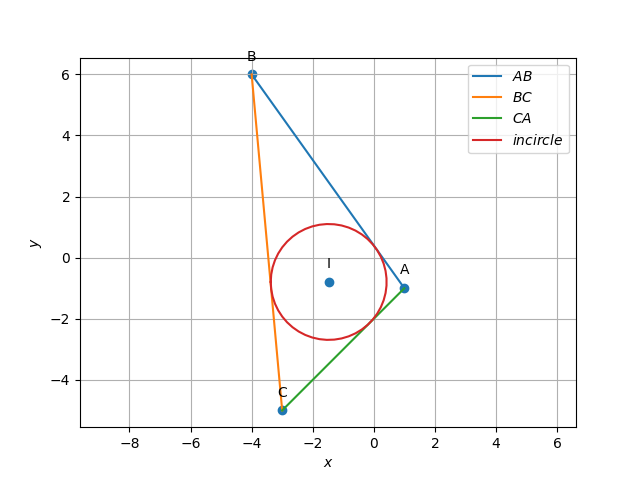
\includegraphics[width=\columnwidth]{solutions/1/5/7/figs/Diagram.png}
	\caption{Triangle with the incircle generated using python}
	\label{fig:Incircle}
\end{figure}

	The equation of the incircle is given as :

	\begin{align}
			\norm{\vec{x}-\vec{I}}^2 = r^2
	\end{align}

	\item Find the intersection $\vec{G}$ of $BE$ and $CF$.
 \\
\solution 
From 
	\eqref{eq:median-be}
	and
	\eqref{eq:median-cf},
the equations of $BE$ 
and 
$CF$
are, respectively,
\begin{align}
\myvec{3 & 1} \vec{x} &= \myvec{-6}
\label{eq:1.2.3,8}
\\
\myvec{ 5&-1} \vec{x} &= \myvec{-10}
\label{eq:1.2.3,9}
\end{align}
From \eqref{eq:1.2.3,8} and \eqref{eq:1.2.3,9} the augmented matrix is
\begin{align}
    \label{eq:matrowoperations}
    \myvec{
    3 & 1 & -6
    \\
    5 & -1 & -10
    }
     \xleftrightarrow[]{R_1 \leftarrow R_1+R_2}
    \myvec{
    8 & 0 & -16
    \\
    5 & -1 & -10 
    }
    \\
     \xleftrightarrow[]{R_1\leftarrow R_1/8}
    \myvec{
    1 & 0 & -2
    \\
    5 & -1 & -10 
    }
     \xleftrightarrow[]{R_2\leftarrow R_2-5R_1}
    \myvec{
    1 & 0 & -2
    \\
    0 & -1 & 0
    }
    \\
     \xleftrightarrow[]{R_2\leftarrow -R_2}
    \myvec{
    1 & 0 & -2
    \\
    0 & 1 & 0
    }
\end{align} 
using Gauss elimination.  Therefore, 
\begin{align}
\vec{G} = \myvec{-2 \\ 0}
	\label{eq:median-g}
\end{align}

	\item Verify that 
		\begin{align}
			\frac{BG}{GE} = 
			\frac{CG}{GF} =
			\frac{AG}{GD} =2 
		\end{align}
		\\	\solution 
\begin{enumerate}
\item From 
	\eqref{eq:median-e}
	and
	\eqref{eq:median-g},
\begin{align}
		\label{eq:tri-pts/4} \vec{G}-\vec{B} &= \myvec{2 \\ -6},\, 
 \vec{E}-\vec{G} = \myvec{1 \\ -3} \\
	\implies \vec{G}-\vec{B} &= 2 \brak{ \vec{E}-\vec{G} }
	\\
	\text{or, }		\label{eq:tri-pts/8}\frac{BG}{GE} &=  2  
\end{align}		
\item Calculating the ratio of $GF$ and $CG$,
\begin{align}
		\label{eq:tri-pts/9} \vec{F}-\vec{G} &= \myvec{\frac{1}{2} \\ \frac{5}{2}} \\
		\label{eq:tri-pts/10} \vec{G}-\vec{C} &= \myvec{1 \\ 5} \\
		\label{eq:tri-pts/11} \norm{\vec{F}-\vec{G}} &= \sqrt{\brak{\frac{1}{2}}^{2} + \brak{\frac{5}{2}}^{2}} &= \frac{\sqrt{26}}{2} \\  
		\label{eq:tri-pts/12} \norm{\vec{G}-\vec{C}} &= \sqrt{1^2 + 5^2} &= \sqrt{26} \\
		\label{eq:tri-pts/13}\frac{CG}{GF} &= \frac{\norm{\vec{G}-\vec{C}}}{\norm{\vec{F}-\vec{G}}} &= \frac{\sqrt{26}}{\frac{\sqrt{26}}{2}} &= 2		
\end{align}
\item Calculating the ratio of $AG$ and $GD$,
\begin{align}
		\label{eq:tri-pts/14} \vec{G}-\vec{A} &= \myvec{-3 \\ 1} \\
		\label{eq:tri-pts/15} \vec{D}-\vec{G} &= \myvec{\frac{-3}{2} \\ \frac{1}{2}} \\
		\label{eq:tri-pts/16} \norm{\vec{G}-\vec{A}} &= \sqrt{\brak{-3}^{2}+1^2} &= \sqrt{10} \\
		\label{eq:tri-pts/17} \norm{\vec{D}-\vec{G}} &= \sqrt{\brak{\frac{-3}{2}}^{2}+\brak{\frac{1}{2}}^{2}} &= \frac{\sqrt{10}}{2} \\
		\label{eq:tri-pts/18}\frac{AG}{GD} &= \frac{\norm{\vec{G}-\vec{A}}}{\norm{\vec{D}-\vec{G}}} &= \frac{\sqrt{10}}{\frac{\sqrt{10}}{2}} &= 2 
\end{align}
\end{enumerate}
From \eqref{eq:tri-pts/8}, \eqref{eq:tri-pts/13}, \eqref{eq:tri-pts/18}
\begin{align}
		\frac{BG}{GE} = 
		\frac{CG}{GF} =
		\frac{AG}{GD} = 2
\end{align}
Hence verified.

	\item Show that $\vec{A}, \vec{G}$ and $\vec{D}$ are collinear.
	\\
		\solution 
Points $\vec{A},\vec{D},\vec{G}$ are defined to be collinear if 
\begin{align}
    \text{rank}\myvec{
    1 & 1 & 1\\
    \vec{A} & \vec{D} & \vec{G} \\
    } = 2 
    \label{eq:mat_row_operations}
    \\
\implies    
    \myvec{
    1 & 1 & 1
    \\
    1 & -\frac{7}{2} & -2
    \\
    -1 & \frac{1}{2} & 0
    }
     \xleftrightarrow[]{R_3 \leftarrow R_3+R_2}
    \myvec{
    1 & 1 & 1
    \\
    1 & -\frac{7}{2} & -2
    \\
    0 & -3 & -2 
    }
    \\
     \xleftrightarrow[]{R_2\leftarrow R_2-R_1}
    \myvec{
    1 & 1 & 1
    \\
    0 & -\frac{9}{2} & -3
    \\
    0 & -3 & -2 
    }
     \xleftrightarrow[]{R_3\leftarrow R_3-\frac{2}{3}R_2}
    \myvec{
    1 & 1 & 1
    \\
    0 & -\frac{9}{2} & -3
    \\
    0 & 0 & 0
    }
\end{align}
Thus, the matrix 
    \eqref{eq:mat_row_operations}
    has rank 2 and the points are collinear.

	\item Verify that 
		\begin{align}
			\vec{G}=\frac{\vec{A}+\vec{B}+\vec{C}}{3}
		\end{align}
			$\vec{G}$ is known as the {\em centroid} of $\triangle ABC$.
   \\
		\solution
\begin{equation}
\begin{split}
\label{eq:centroid}
    \vec{G}&= \frac{\myvec{1\\-1}+\myvec{-4\\6}+\myvec{-3\\-5}}{3}\\    
     &= \myvec{-2\\0}
\end{split}
\end{equation}

 




	\item Verify that 
		\begin{align}
\vec{A}-\vec{F}=\vec{E}-\vec{D}
		\end{align}
		The quadrilateral $AFDE$ is defined to be a parallelogram.\\
  		\\ \solution 
\begin{align}
    \vec{A}-\vec{F}&=\myvec{1\\-1}-\myvec{\frac{-3}{2}\\\frac{5}{2}}
    =\myvec{\frac{5}{2}\\\frac{-7}{2}}
    \\
    \vec{E}-\vec{D}&=\myvec{-1\\-3}-\myvec{\frac{-7}{2}\\\frac{1}{2}}
    =\myvec{\frac{5}{2}\\\frac{-7}{2}}
    \\
	\implies	\vec{A}-\vec{F} &= \vec{E}-\vec{D}
\end{align}
See \figref{fig:Triangle}, 
\begin{figure}
\centering
\includegraphics[width=\columnwidth]{solutions/1/2/7/figs/figure1.png}
\caption{$AFDE$ form a parallelogram in triangle ABC}
\label{fig:Triangle}
\end{figure}






















  
\end{enumerate}

\section{Altitude}
%\renewcommand{\theequation}{\theenumi}
%\begin{enumerate}[label=\arabic*.,ref=\theenumi]
\begin{enumerate}[label=\thesection.\arabic*.,ref=\thesection.\theenumi]
\numberwithin{equation}{enumi}
\item $\vec{D}_1$ is a point on $BC$ such that
		\begin{align}
			AD_1 \perp BC
		\end{align}
		and $AD_1$ is defined to be the altitude. 
		Find the normal vector of $AD_1$.
  \\
		\solution
The normal vector of $AD_{1}$ 
is
the direction vector $BC$ and is obtained from  
		\eqref{eq:geo-dir-vec-bc}
		as
\begin{align}
	\vec{n} = 
\myvec{1\\-11}
\end{align}


	\item Find the equation of $AD_1$.
 \\     \solution
The equation of $AD_1$ is
\begin{align}
 \vec{n}^{\top}(\vec{x-A}) &= 0 \\
\implies \myvec{-1 & 11}\vec{x} &= \myvec{-1 & 11}\myvec{1 \\ -1}
= -12
\end{align}


	\item Find the equations of the altitudes $BE_1$ and $CF_1$ to the sides $AC$ and $AB$ respectively. 
  \\     \\ \solution
\begin{enumerate}
\item 
	From 
		\eqref{eq:geo-dir-vec-ca},
the normal vector of $CF_1$ is 
\begin{align}
\vec{n}&=\myvec{-5\\7} 
\end{align}
and the equation of $CF_1$ is
\begin{align}
\vec{n}^{\top}\brak{\vec{x}-\vec{C}}&=0 \\
\implies 
\myvec{-5 & 7}\brak{\vec{x}-\myvec{-3\\-5}}&=0  \\
	\implies \myvec{5 & 7}\vec{x}&=20
		\label{eq:geo-alt-cf},
\end{align}
\item Similarly, 
	from 
		\eqref{eq:geo-dir-vec-ab},
the normal vector of $BE_1$ is 
\begin{align}
\vec{n}= \myvec{1 \\1}
\end{align}
and the equation of  $BE_1$ is
\begin{align}
\vec{n}^{\top}\brak{\vec{x}-\vec{B}}&=0 \\
\implies \myvec{1 \\1}^\top\brak{\vec{x}-\myvec{-4\\6}}&=0 \\
	\implies \myvec{1 & 1}\vec{x}&=2
		\label{eq:geo-alt-be},
\end{align}
\end{enumerate}



	\item Find the intersection $\vec{H}$ of $BE_1$ and $CF_1$.
 \\
        \\ \solution
%
The intersection of 
		\eqref{eq:geo-alt-be}
		and
		\eqref{eq:geo-alt-cf},
		is obtained from 
		the matrix equation
		%
\begin{align}
        \myvec{1&1\\5&-7} \vec{x} &= \myvec{2\\20}
\end{align}
%
which can be solved as 
%
\begin{align}
        \myvec{1&1&2\\5&-7&20}
	 \xleftrightarrow[]{R_2 \leftarrow R_2 - 5R_1}
        \myvec{1&1&2\\0&-12&10}\\
	 \xleftrightarrow[]{R_2 \leftarrow \frac{R_2}{-12}}
        \myvec{1&1&2\\0&1&\frac{-5}{6}}
	 \xleftrightarrow[]{R_1 \leftarrow R_1 - R_2}
        \myvec{1&0&\frac{17}{6}\\0&1&\frac{-5}{6}}
\end{align}
%
yielding
%
\begin{align}
        \vec{H}&=\frac{1}{6}\myvec{{17}\\-{5}}
		\label{eq:geo-alt-H},
\end{align}
%
See 
\figref{fig:m_tri_py}
\begin{figure}[!ht]
\centering
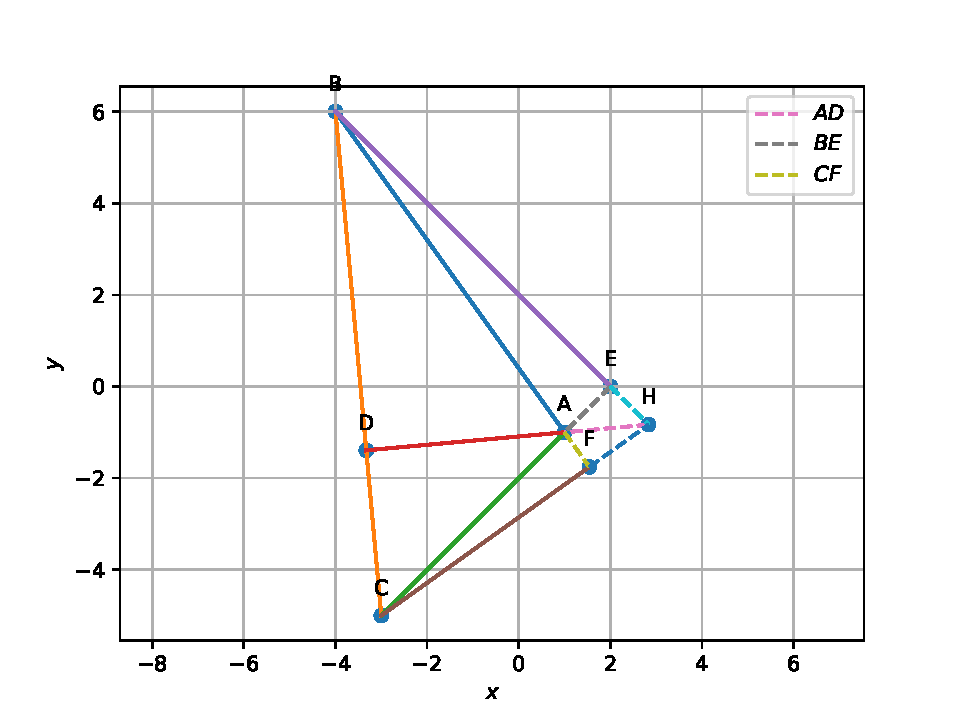
\includegraphics[width=\columnwidth]{figs/triangle/altitude.pdf}
\caption{Altitudes $BE_1$ and $CF_1$ intersect at $\vec{H}$}
\label{fig:m_tri_py}
\end{figure}


	\item Verify that 
		\begin{align}
			\brak{\vec{A}-\vec{H}}^{\top}\brak{\vec{B}-\vec{C}} = 0
		\end{align}
  \solution
From 
		\eqref{eq:geo-alt-H},
\begin{align}
\vec{A}-\vec{H}=-\frac{1}{6}\myvec{{11}\\{1}},\,
\vec{B}-\vec{C}=\myvec{-1\\11}
\\
	\implies \brak{\vec{A}-\vec{H}}^{\top}\brak{\vec{B}-\vec{C}}=\frac{1}{6}\myvec{11 & 1}
\myvec{-1\\11}
=0
\end{align}


\end{enumerate}

\section{Perpendicular Bisector}
%\renewcommand{\theequation}{\theenumi}
%\begin{enumerate}[label=\arabic*.,ref=\theenumi]
\begin{enumerate}[label=\thesection.\arabic*.,ref=\thesection.\theenumi]
\numberwithin{equation}{enumi}

\item The equation of the perpendicular bisector of $BC$ is
		\begin{align}
			\label{eq:tri-perp-bisect}
			\brak{\vec{x}-\frac{\vec{B}+\vec{C}}{2}}\brak{\vec{B}-\vec{C}} = 0
		\end{align}
		Substitute numerical values and find the equations of the perpendicular bisectors of $AB, BC$ and $CA$.
	\\	\solution
From 
		\eqref{eq:geo-dir-vec-ab},
		\eqref{eq:geo-dir-vec-bc},
		\eqref{eq:geo-dir-vec-ca},
	\eqref{eq:median-d},
	\eqref{eq:median-e}
	and
	\eqref{eq:median-f},
\begin{align}
\vec{\frac{\vec{B}+\vec{C}}{2}} &= \frac{1}{2}\myvec{-{7} \\ 1},\,
\vec{B}-\vec{C} = \myvec{-1 \\ 11} 
\\
\vec{\frac{\vec{A}+\vec{B}}{2}}&=\frac{1}{2}\myvec{-{3} \\{5}},\,
\vec{A}-\vec{B}=\myvec{5\\ -7} \\
\vec{\frac{\vec{C}+\vec{A}}{2}} &= \myvec{-1\\-3},\,
\vec{C}-\vec{A} = \myvec{-4\\-4} \\
\end{align}
yielding
\begin{alignat}{2}
  \brak{\vec{B}-\vec{C}}^{\top}\brak{\frac{\vec{B}+\vec{C}}{2}}
	&=\myvec{-1&11}\myvec{-\frac{7}{2} \\ \frac{1}{2}}
	&&=9
  \\
\brak{\vec{A}-\vec{B}}^{\top}\brak{\frac{\vec{A}+\vec{B}}{2}}
	&=\myvec{5&-7}\myvec{-\frac{3}{2} \\\frac{5}{2}}
	&&=-25
  \\
\brak{\vec{C}-\vec{A}}^{\top}\brak{\frac{\vec{C}+\vec{A}}{2}}
	&=\myvec{-4&-4}\myvec{-1\\-3}
	&&=16
\end{alignat}
Thus, the perpendicular bisectors are obtained from 
			\eqref{eq:tri-perp-bisect}
			as
		\begin{alignat}{2}
			BC&: \quad \myvec{-1&11}\vec{x}&&=9
\\
			CA&: \quad \myvec{5&-7}\vec{x}&&=-25
\\
			AB&: \quad \myvec{-4&-4}\vec{x}&&=16
		\end{alignat}
\begin{figure}
\centering
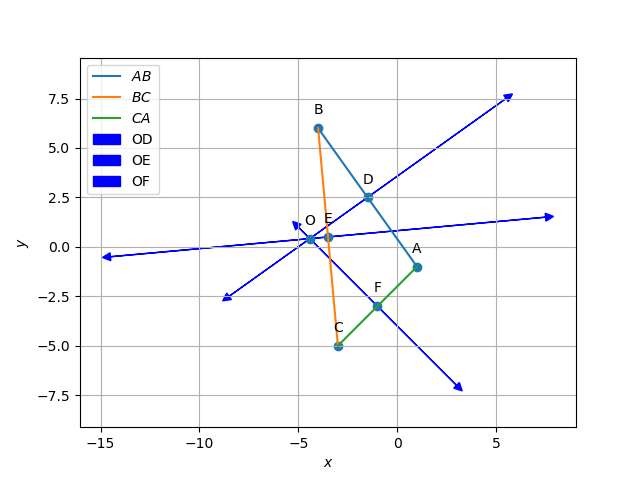
\includegraphics[width=\columnwidth]{solutions/1/4/1/figs/trianglecircum.png}
\caption{Plot of the perpendicular bisectors}
\label{fig:figure1}
\end{figure}




	\item Find the intersection $\vec{O}$ of the perpendicular bisectors of $AB$ and $AC$.
 \\
 \solution \\
The intersection of 
			\eqref{eq:tri-perp-bisect-ca}
			and
			\eqref{eq:tri-perp-bisect-ab},
			can be obtained as
\begin{align}
\myvec{5&-7&-25\\1&1&-4} \xleftrightarrow[]{R_2 \leftarrow 5R_2 - R_1} \myvec{5&-7&-25\\0&12&5}\\
 \xleftrightarrow[]{R_1\leftarrow \frac{12}{7}R_1 + R_2} \myvec{\frac{60}{7}&0& \frac{-265}{7}\\0&12&5}
 \xleftrightarrow[R_1\leftarrow \frac{7}{60}R_1]{R_2 \leftarrow \frac{1}{12}R_2} \myvec{1&0& \frac{-53}{12}\\0&1&\frac{5}{12}}\\
\implies \vec{O}=\myvec{\frac{-53}{12}\\\frac{5}{12}}
			\label{eq:tri-perp-bisect-O}
\end{align}

	\item Verify that $\vec{O}$ satisfies
			\eqref{eq:tri-perp-bisect}.
$\vec{O}$ is known as the circumcentre.\\
    \solution
Substituing  from 
			\eqref{eq:tri-perp-bisect-O} in 
			\eqref{eq:tri-perp-bisect},
when substituted in the above equation,
\begin{multline}
	\brak{\vec{O}-\frac{\vec{B}+\vec{C}}{2}}^{\top}\brak{\vec{B}-\vec{C}}\\
	=\brak{\frac{1}{12}\myvec{-53\\5}- \frac{1}{2}\myvec{-7\\1}}^{\top} \myvec{-1\\11}\\
	=\frac{1}{12}\myvec{-11&-1}\myvec{-1\\11}
	=0
\end{multline}




		\item Verify that 
		\begin{align}
			OA = OB = OC 
		\end{align}
                \solution
\begin{align}
      R &= OA\\
        &= \norm{\vec{A} - \vec{O}}\\
        &= \norm{\myvec{1\\-1} - \frac{1}{12}\myvec{-53\\5}}\\
        &= \norm{\frac{1}{12}\myvec{65\\-17}}\\
        &= \frac{\sqrt{4514}}{12}
\end{align}


	\item Draw the circle with centre at $\vec{O}$ and radius 
		\begin{align}
			R = OA
		\end{align}
		This is known as the {\em circumradius}. 
  \\  \solution 
See 
\figref{fig:circumcircle with centre O}.
\begin{figure}
\centering
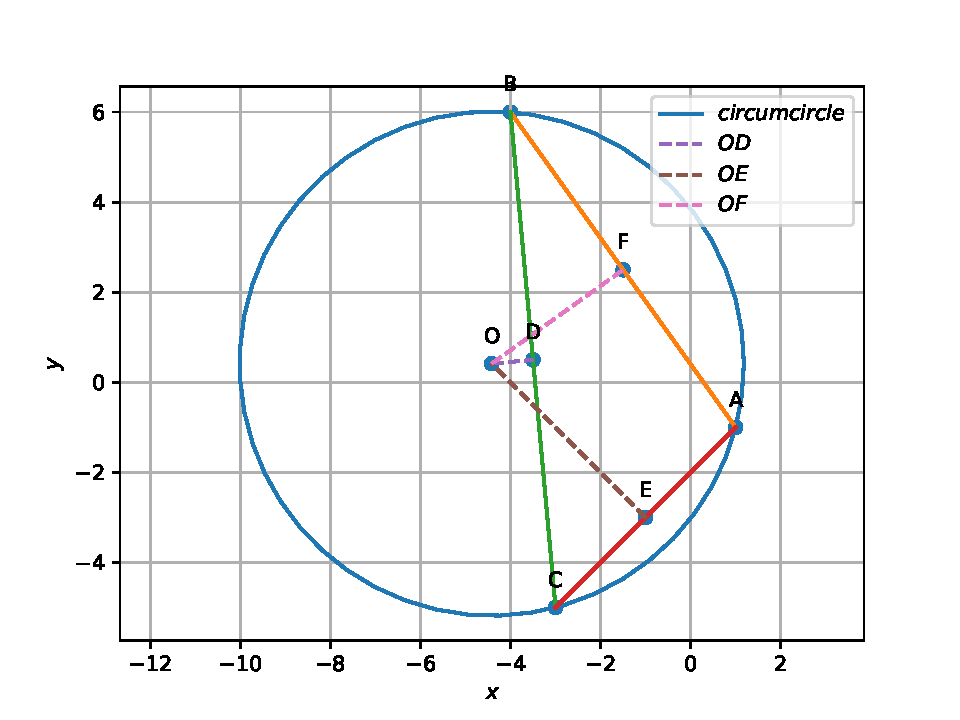
\includegraphics[width=\columnwidth]{figs/triangle/perp-bisect.pdf}
	\caption{Circumcircle of $\triangle ABC$ with centre $\vec{O}$.}
\label{fig:circumcircle with centre O}	
\end{figure}


	\item Verify that 
		\begin{align}
			\angle BOC = 2\angle BAC.
		\end{align}\\
  \solution
\begin{enumerate}
\item To find  the value of $\angle{BOC}$ :
\begin{align}
\vec{B}-\vec{O}
          &=\myvec{\frac{5}{12}\\\frac{67}{12}},\,
\vec{C}-\vec{O}
          =\myvec{\frac{17}{12}\\\frac{-65}{12}}
	  \\
\implies \brak{\vec{B}-\vec{O}}^{\top}\brak{\vec{C}-\vec{O}}&=\frac{-4270}{144}\\
	\implies \norm{\vec{B}-\vec{O}}&= \frac{\sqrt{4514}}{12},\,
	\norm{\vec{C}-\vec{O}}= \frac{\sqrt{4514}}{12}
\end{align}
Thus,
\begin{align}
\cos{BOC}&=\frac{\brak{\vec{B}-\vec{O}}^{\top}\brak{\vec{C}-\vec{O}}}{\norm{\vec{B}-\vec{O}}\norm{\vec{C}-\vec{O}}}
=\frac{-4270}{4514}\\
\implies\angle{BOC}&=\cos^{-1}\brak{\frac{-4270}{4514}}
\\
	&=161.07536\degree
	\text{ or }
	198.92464\degree\label{eq:1}
\end{align}
	\item To find  the value of $\angle{BAC}$ :
\begin{align}
\vec{B}-\vec{A}&=\myvec{-5\\7},\,
\vec{C}-\vec{A}=\myvec{-4\\-4}
\\
\implies \brak{\vec{B}-\vec{A}}^{\top}\brak{\vec{C}-\vec{A}}&=-8
\\
	\norm{\vec{B}-\vec{A}}&= \sqrt{74}
	\norm{\vec{C}-\vec{A}}= 4\sqrt{2}
\end{align}
Thus,
\begin{align}
\cos{BAC}&=\frac{\brak{\vec{B}-\vec{A}}^{\top}\brak{\vec{C}-\vec{A}}}{\norm{\vec{B}-\vec{A}}\norm{\vec{C}-\vec{A}}}
=\frac{-8}{4\sqrt{148}}\\
\implies\angle{BAC}&=\cos^{-1}\brak{\frac{-8}{4\sqrt{148}}}\\
&=99.46232\degree \label{eq:2}
\end{align}
From \eqref{eq:2} and \eqref{eq:1},
\begin{align}
2\times\angle{BAC}
= \angle{BOC}
\end{align}
\end{enumerate}





	\item Let 
		\begin{align}
			\vec{P} = \myvec{\cos \theta & -\sin \theta \\ \sin \theta & \cos \theta}
		\end{align}
		Find $\theta$ if 
		\begin{align}
			\vec{C}-\vec{O}=\vec{P}\brak{\vec{A}-\vec{O}}
		\end{align}
\end{enumerate}

\section{Angle Bisector}
%\renewcommand{\theequation}{\theenumi}
%\begin{enumerate}[label=\arabic*.,ref=\theenumi]
\begin{enumerate}[label=\thesection.\arabic*.,ref=\thesection.\theenumi]
\numberwithin{equation}{enumi}
	\item Let $\vec{D}_3, \vec{E}_3, \vec{F}_3$, be points on $AB, BC$ and $CA$ respectively such that
		\begin{align}
			BD_3 = BF_3=m, CD_3 = CE_3=n, AE_3 = AF_3=p.
		\end{align}
	Obtain $m,n,p$ in terms of $a,b,c$ obtained in  
		\probref{prob:side-length}.
 \\
 		\solution 
From the given information, 
\begin{align}
% 
    a &= m+n,\\
    b &= n+p, \\
    c &= m+p 
\end{align}
which can be expressed as
\begin{align}
\myvec{1&1&0\\0&1&1\\1&0&1\\}\myvec{m\\n\\p} &= \myvec{a\\b\\c}
\\
\implies 
	\myvec{m\\n\\p} &= \myvec{1&1&0\\0&1&1\\1&0&1\\}^{-1}\myvec{a\\b\\c}
\end{align}
Using row reduction,
		\begin{align}
			\augvec{3}{3}{1&1&0 & 1 & 0 & 0\\0&1&1 & 0 & 1 & 0\\1&0&1 & 0 & 0 & 1}
			\xleftrightarrow[]{R_3 \leftarrow R_3 - R_1}
			\augvec{3}{3}{1&1&0 & 1 & 0 & 0\\0&1&1 & 0 & 1 & 0\\0&-1&1 & -1 & 0 & 1}
		\end{align}
		\begin{align}
			\xleftrightarrow[R_1 \leftarrow R_1 - R_2]{R_3 \leftarrow R_3 + R_2}
			\augvec{3}{3}{1&0&-1 & 1 & -1 & 0\\0&1&1 & 0 & 1 & 0\\0&0&2 & -1 & 1 & 1}
		\end{align}
		\begin{align}
			\xleftrightarrow[R_1 \leftarrow 2R_1 + R_3]{R_2 \leftarrow 2R_2 - R_3}
			\augvec{3}{3}{2&0&0 & 1 & -1 & 1\\0&2&0 & 1 & 1 & -1\\0&0&2 & -1 & 1 & 1}
		\end{align}
yielding
		\begin{align}
			\myvec{1&1&0\\0&1&1\\1&0&1\\}^{-1} = 
			\frac{1}{2}\myvec{1 & -1 & 1\\ 1 & 1 & -1\\ -1 & 1 & 1}
		\end{align}
	Therefore,
\begin{align}
\begin{split}
    p&=\frac{c+b-a}{2}
    =\frac{\sqrt{74}+\sqrt{32}-\sqrt{122}}{2}
    \\
    m&=\frac{a+c-b}{2}
    =\frac{\sqrt{74}+\sqrt{122}-\sqrt{32}}{2}
    \\
    n&=\frac{a+b-c}{2}
    =\frac{\sqrt{122}+\sqrt{32}-\sqrt{74}}{2}
\end{split}
	\label{eq:incircle-mnp}
\end{align}
upon substituting from 
		\eqref{eq:geo-norm-ab},
		\eqref{eq:geo-norm-bc}
		and
		\eqref{eq:geo-norm-ca}.

	\item Using section formula, find 
		\begin{align}
			\vec{D}_3 = \frac{m\vec{C}+n\vec{B}}{m+n},\,
			\vec{E}_3 = \frac{n\vec{A}+p\vec{C}}{n+p},\,
			\vec{F}_3 = \frac{p\vec{B}+m\vec{A}}{p+m}
		\end{align}
	\item Find the circumcentre and circumradius of $\triangle D_3E_3F_3$.  These are the {\em incentre} and {\em inradius} of $\triangle ABC$.
	\item Draw the circumcircle of $\triangle D_3E_3F_3$.  This is known as the {\em incircle} of $\triangle ABC$.
		\\
 		\solution
Considering
\begin{align}
	BC: \quad \vec{n} ^\top \vec{x} &= c, 
\end{align}
the distance from $\vec{I}$ to $BC$ is 
\begin{align}
\frac{\abs{\vec{n}^\top \vec{I} - c}}{\norm{\vec{n}}} 
\end{align}


	\item Using 
    \eqref{eq:angle2d}
verify that 
		\begin{align}
			\angle BAI = \angle CAI.
		\end{align}
		$AI$ is the bisector of $\angle A$.  
	\item Verify that $BI, CI$ are also the angle bisectors of $\triangle ABC$.

		\iffalse

\item Suppose the equations  given by 
		\begin{align}
			\label{eq:tri-sides}
			\vec{n}_i^{\top}\vec{x}=c_i \quad i = 1, 2, 3 
		\end{align}
		The equations of the respective angle bisectors are then given by 
		\begin{align}
			\frac{\vec{n}_i^{\top}\vec{x}-c_i}{\norm{\vec{n}_i}}
		=
	\pm	\frac{\vec{n}_j^{\top}\vec{x}-c_j}{\norm{\vec{n}_j}}
\quad i \ne j
		\end{align}
		Substitute numerical values and find the equations of the angle bisectors of $A, B$ and $C$.
	\\
		%\textbf{Solution :}
	The parametric equations of sides;
	\begin{align}
	BC:\quad &\myvec{11&1}\vec{x}=-38,\\
	CA:\quad &\myvec{1&-1}\vec{x}=2,\\
	AB:\quad &\myvec{7&5}\vec{x}=2\\	  
	\end{align}
	Using the formula mentioned in the question to find out the angular bisector for sides \text{AB} and \text{AC}, naming the angular bisector $L$ we get,
	\begin{align}
		\frac{\vec{n}_{3}^{\top} \vec{x}-c_{3}}{\norm{\vec{n}_{3}}}=\pm \frac{\vec{n}_{2}^{\top} \vec{x}-c_{2}}{\norm{\vec{n}_{2}}}
	\end{align}
	\begin{figure}
	\centering
	\includegraphics[width=\columnwidth]{solutions/1/5/1/figs/angular_bisector.png}
	\caption{Triangle generated using python}
	\label{fig:angular_bisector}
	\end{figure}
	As we can see we will get 2 solutions for $L$. This is because one of them is internal angular bisector and the other is the external angular bisector. Internal angular bisector can be evaluated if we take + in the above formula.
	Hence, $L$ is given by,
	\begin{align}
		\frac{\vec{n}_{3}^{\top} \vec{x}-c_{3}}{\norm{\vec{n}_{3}}}&=\frac{\vec{n}_{2}^{\top} \vec{x}-c_{2}}{\norm{\vec{n}_{2}}}\\
		\implies \brak{\frac{\vec{n_{3}}}{\norm{\vec{n_{3}}}}-\frac{\vec{n_{3}}}{\norm{\vec{n_{3}}}}} \vec{x}&=\brak{\frac{c_{3}}{\norm{\vec{n_{3}}}}-\frac{c_{2}}{\norm{\vec{n_{2}}}}}\\
		\implies \brak{\frac{\myvec{7&5}}{\sqrt{74}}-\frac{\myvec{1&-1}}{\sqrt{2}}} \vec{x}&=\frac{2}{\sqrt{74}}-\frac{2}{\sqrt{2}}\\
		\implies \myvec{\frac{7-\sqrt{37}}{\sqrt{74}}&\frac{5+\sqrt{37}}{\sqrt{74}}}\vec{x}&=\frac{2-2\sqrt{37}}{\sqrt{74}}
	\end{align}
	Hence, the internal angluar bisector of angle $A$, $L$ will be,
	\begin{align}
		\implies\myvec{\frac{7-\sqrt{37}}{\sqrt{74}}&\frac{5+\sqrt{37}}{\sqrt{74}}} \vec{x}=\frac{2-2\sqrt{37}}{\sqrt{74}}
		\label{eq:1.5.1}
	\end{align}
	

  \solution 
The above formula can 
be transformed to the normal equation of angle bisectors as  
\begin{align}
       \myvec{\frac{\vec{n}_i}{\norm{\vec{n}_i}} - \frac{\vec{n}_j}{\norm{\vec{n}_j}}}^{\top}\vec{x}
       =
       \frac{c_i}{\norm{\vec{n}_i}}-\frac{c_j}{\norm{\vec{n}_j}}
\end{align}
\begin{enumerate}
\item From 
		\eqref{eq:geo-norm-vec-ab}
		and 
		\eqref{eq:geo-norm-vec-ca}
the angle Bisector of $A$ is 
\begin{align}
\myvec{
\frac{7}{\sqrt{74}}-\frac{1}{\sqrt{2}} & \frac{5}{\sqrt{74}}+\frac{1}{\sqrt{2}}\\
}
\vec{x}
=\frac{2}{\sqrt{74}}-\frac{2}{\sqrt{2}}
\end{align}
\item Similarly, the angle bisector of $B$ is 
\begin{align}
\myvec{
\frac{11}{\sqrt{122}}+\frac{7}{\sqrt{74}} & \frac{1}{\sqrt{122}}+\frac{5}{\sqrt{74}}\\
}
\vec{x}
=\frac{2}{\sqrt{74}}-\frac{38}{\sqrt{122}}
\end{align}
\item and the angle bisector of $C$ is 
\begin{align}
\myvec{
\frac{11}{\sqrt{122}}+\frac{1}{\sqrt{2}} & \frac{1}{\sqrt{122}}-\frac{1}{\sqrt{2}}\\
}
\vec{x}
=\frac{2}{\sqrt{2}}-\frac{38}{\sqrt{122}}
\end{align}
\end{enumerate}

	\item Find the intersection $\vec{I}$ of the angle bisectors of $B$ and $C$.
	\item Find the distance from $\vec{I}$ to $BC$.  
  \\
		\solution
Considering
\begin{align}
	BC: \quad \vec{n} ^\top \vec{x} &= c, 
\end{align}
the distance from $\vec{I}$ to $BC$ is 
\begin{align}
\frac{\abs{\vec{n}^\top \vec{I} - c}}{\norm{\vec{n}}} 
\end{align}

 
	\item Repeat the above exercise for the sides $AB$ and $AC$.
	This distance is known as the {\em inradius} $r$.
	\item Draw a circle with center $\vec{I}$ and radius $r$.  $\vec{I}$ is known as the {\em incentre}.
	\item The equation of the {\em incircle} is given by 
		\begin{align}
			\label{eq:incircle}
			\norm{\vec{x}-\vec{I}}^2 = r^2
		\end{align}
		Using the parameteric equation of $BC$, verify that $BC$ intersects the incircle at exactly one point. $BC$ is defined to be a {\em tangent} to the incircle.
		\\
		\iffalse
\let\negmedspace\undefined
\let\negthickspace\undefined
\documentclass[journal,12pt,twocolumn]{IEEEtran}
\usepackage{cite}
\usepackage{amsmath,amssymb,amsfonts,amsthm}
\usepackage{algorithmic}
\usepackage{graphicx}
\usepackage{textcomp}
\usepackage{xcolor}
\usepackage{txfonts}
\usepackage{listings}
\usepackage{enumitem}
\usepackage{mathtools}
\usepackage{gensymb}
\usepackage[breaklinks=true]{hyperref}
\usepackage{tkz-euclide} % loads  TikZ and tkz-base
\usepackage{listings}
\usepackage{gvv}
%
%\usepackage{setspace}
%\usepackage{gensymb}
%\doublespacing
%\singlespacing

%\usepackage{graphicx}
%\usepackage{amssymb}
%\usepackage{relsize}
%\usepackage[cmex10]{amsmath}
%\usepackage{amsthm}
%\interdisplaylinepenalty=2500
%\savesymbol{iint}
%\usepackage{txfonts}
%\restoresymbol{TXF}{iint}
%\usepackage{wasysym}
%\usepackage{amsthm}
%\usepackage{iithtlc}
%\usepackage{mathrsfs}
%\usepackage{txfonts}
%\usepackage{stfloats}
%\usepackage{bm}
%\usepackage{cite}
%\usepackage{cases}
%\usepackage{subfig}
%\usepackage{xtab}
%\usepackage{longtable}
%\usepackage{multirow}
%\usepackage{algorithm}
%\usepackage{algpseudocode}
%\usepackage{enumitem}
%\usepackage{mathtools}
%\usepackage{tikz}
%\usepackage{circuitikz}
%\usepackage{verbatim}
%\usepackage{tfrupee}
%\usepackage{stmaryrd}
%\usetkzobj{all}
%    \usepackage{color}                                            %%
%    \usepackage{array}                                            %%
%    \usepackage{longtable}                                        %%
%    \usepackage{calc}                                             %%
%    \usepackage{multirow}                                         %%
%    \usepackage{hhline}                                           %%
%    \usepackage{ifthen}                                           %%
  %optionally (for landscape tables embedded in another document): %%
%    \usepackage{lscape}     
%\usepackage{multicol}
%\usepackage{chngcntr}
%\usepackage{enumerate}

%\usepackage{wasysym}
%\documentclass[conference]{IEEEtran}
%\IEEEoverridecommandlockouts
% The preceding line is only needed to identify funding in the first footnote. If that is unneeded, please comment it out.

\newtheorem{theorem}{Theorem}[section]
\newtheorem{problem}{Problem}
\newtheorem{proposition}{Proposition}[section]
\newtheorem{lemma}{Lemma}[section]
\newtheorem{corollary}[theorem]{Corollary}
\newtheorem{example}{Example}[section]
\newtheorem{definition}[problem]{Definition}
%\newtheorem{thm}{Theorem}[section] 
%\newtheorem{defn}[thm]{Definition}
%\newtheorem{algorithm}{Algorithm}[section]
%\newtheorem{cor}{Corollary}
\newcommand{\BEQA}{\begin{eqnarray}}
\newcommand{\EEQA}{\end{eqnarray}}
\newcommand{\define}{\stackrel{\triangle}{=}}
\theoremstyle{remark}
\newtheorem{rem}{Remark}

%\bibliographystyle{ieeetr}
\begin{document}
%

\bibliographystyle{IEEEtran}


\vspace{3cm}

\title{
Question 1.5.7
}
\author{ SREEKAR CHEELA - EE22BTECH11051$^{*}$% <-this % stops a space
	\thanks{*The author is with the Department
		of Electrical Engineering, Indian Institute of Technology, Hyderabad
		502285 India e-mail:  ee22btech11051@iith.ac.in. All content in this manual is released under GNU GPL.  Free and open source.}
	
}	
% make the title area
\maketitle

\newpage

\bigskip

\renewcommand{\thefigure}{\theenumi}
\renewcommand{\thetable}{\theenumi}
%\renewcommand{\theequation}{\theenumi}

%\tableofcontents

% Within an equation environment

\textbf{Question :} Draw a circle with its centre as I (incentre) and radius r (inradius)\\
\fi
\textbf{Solution :}
The vertices of the given triangle are:

\begin{align}
	\vec {A}= &\myvec{1\\-1};\\ \vec {B}= &\myvec{-4\\6};\\ \vec {C}= &\myvec{-3\\-5}
\end{align}

The incentre of the triangle is:

	\begin{align}
	\vec{I}=&\myvec{
		-1.48 \\
		-0.79}
	\end{align}

	The inradius of the triangle is:

    \begin{align}
    r = \frac{185+41\sqrt{37}-37\sqrt{61}-\sqrt{2257}}{6\sqrt{74}} = 1.896\\
    \end{align}
\begin{figure}
	\centering
	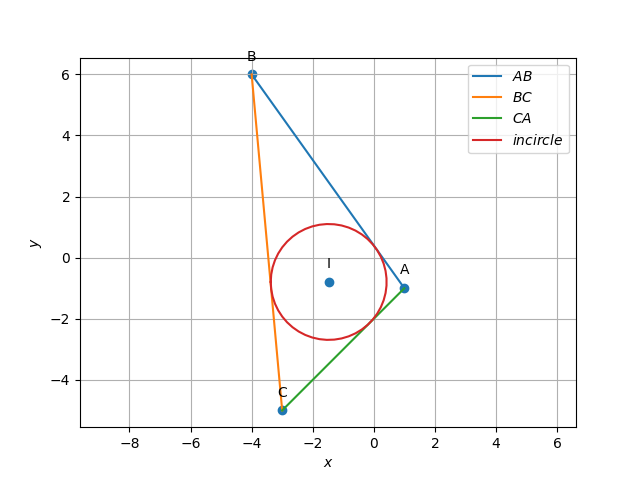
\includegraphics[width=\columnwidth]{solutions/1/5/7/figs/Diagram.png}
	\caption{Triangle with the incircle generated using python}
	\label{fig:Incircle}
\end{figure}

	The equation of the incircle is given as :

	\begin{align}
			\norm{\vec{x}-\vec{I}}^2 = r^2
	\end{align}

	\item Find the {\em point of contact} $\vec{D}_3$ where $BC$ touches the incircle.
		\\
		\solution
Since
	\eqref{eq:incircle-disc}
	has only one root, 
\begin{align}
k=-\frac{\vec{m}^{\top}\brak{\vec{B}-\vec{I}}}{{\ \norm{\vec{m}}^2}}
\end{align}
Substituing the above in 
\eqref{eq:8},
\begin{align}
	\vec{D_{3}} = \vec{B} -\frac{\vec{m}^{\top}\brak{\vec{B}-\vec{I}}}{{\ \norm{\vec{m}}^2}} \vec{m}
\end{align}



  \item Find the other points of contact $\vec{E}_3$ and $\vec{F}_3$.
  \\
		\iffalse
\let\negmedspace\undefined
\let\negthickspace\undefined
\documentclass[journal,12pt,twocolumn]{IEEEtran}
\usepackage{cite}
\usepackage{amsmath,amssymb,amsfonts,amsthm}
\usepackage{algorithmic}
\usepackage{graphicx}
\usepackage{textcomp}
\usepackage{xcolor}
\usepackage{txfonts}
\usepackage{listings}
\usepackage{enumitem}
\usepackage{mathtools}
\usepackage{gensymb}
\usepackage[breaklinks=true]{hyperref}
\usepackage{tkz-euclide} % loads  TikZ and tkz-base
\usepackage{listings}
\usepackage{gvv}
%
%\usepackage{setspace}
%\usepackage{gensymb}
%\doublespacing
%\singlespacing

%\usepackage{graphicx}
%\usepackage{amssymb}
%\usepackage{relsize}
%\usepackage[cmex10]{amsmath}
%\usepackage{amsthm}
%\interdisplaylinepenalty=2500
%\savesymbol{iint}
%\usepackage{txfonts}
%\restoresymbol{TXF}{iint}
%\usepackage{wasysym}
%\usepackage{amsthm}
%\usepackage{iithtlc}
%\usepackage{mathrsfs}
%\usepackage{txfonts}
%\usepackage{stfloats}
%\usepackage{bm}
%\usepackage{cite}
%\usepackage{cases}
%\usepackage{subfig}
%\usepackage{xtab}
%\usepackage{longtable}
%\usepackage{multirow}
%\usepackage{algorithm}
%\usepackage{algpseudocode}
%\usepackage{enumitem}
%\usepackage{mathtools}
%\usepackage{tikz}
%\usepackage{circuitikz}
%\usepackage{verbatim}
%\usepackage{tfrupee}
%\usepackage{stmaryrd}
%\usetkzobj{all}
%    \usepackage{color}                                            %%
%    \usepackage{array}                                            %%
%    \usepackage{longtable}                                        %%
%    \usepackage{calc}                                             %%
%    \usepackage{multirow}                                         %%
%    \usepackage{hhline}                                           %%
%    \usepackage{ifthen}                                           %%
  %optionally (for landscape tables embedded in another document): %%
%    \usepackage{lscape}     
%\usepackage{multicol}
%\usepackage{chngcntr}
%\usepackage{enumerate}

%\usepackage{wasysym}
%\documentclass[conference]{IEEEtran}
%\IEEEoverridecommandlockouts
% The preceding line is only needed to identify funding in the first footnote. If that is unneeded, please comment it out.

\newtheorem{theorem}{Theorem}[section]
\newtheorem{problem}{Problem}
\newtheorem{proposition}{Proposition}[section]
\newtheorem{lemma}{Lemma}[section]
\newtheorem{corollary}[theorem]{Corollary}
\newtheorem{example}{Example}[section]
\newtheorem{definition}[problem]{Definition}
%\newtheorem{thm}{Theorem}[section] 
%\newtheorem{defn}[thm]{Definition}
%\newtheorem{algorithm}{Algorithm}[section]
%\newtheorem{cor}{Corollary}
\newcommand{\BEQA}{\begin{eqnarray}}
\newcommand{\EEQA}{\end{eqnarray}}
\newcommand{\define}{\stackrel{\triangle}{=}}
\theoremstyle{remark}
\newtheorem{rem}{Remark}

%\bibliographystyle{ieeetr}
\begin{document}
%

\bibliographystyle{IEEEtran}


\vspace{3cm}

\title{
Question 1.5.7
}
\author{ SREEKAR CHEELA - EE22BTECH11051$^{*}$% <-this % stops a space
	\thanks{*The author is with the Department
		of Electrical Engineering, Indian Institute of Technology, Hyderabad
		502285 India e-mail:  ee22btech11051@iith.ac.in. All content in this manual is released under GNU GPL.  Free and open source.}
	
}	
% make the title area
\maketitle

\newpage

\bigskip

\renewcommand{\thefigure}{\theenumi}
\renewcommand{\thetable}{\theenumi}
%\renewcommand{\theequation}{\theenumi}

%\tableofcontents

% Within an equation environment

\textbf{Question :} Draw a circle with its centre as I (incentre) and radius r (inradius)\\
\fi
\textbf{Solution :}
The vertices of the given triangle are:

\begin{align}
	\vec {A}= &\myvec{1\\-1};\\ \vec {B}= &\myvec{-4\\6};\\ \vec {C}= &\myvec{-3\\-5}
\end{align}

The incentre of the triangle is:

	\begin{align}
	\vec{I}=&\myvec{
		-1.48 \\
		-0.79}
	\end{align}

	The inradius of the triangle is:

    \begin{align}
    r = \frac{185+41\sqrt{37}-37\sqrt{61}-\sqrt{2257}}{6\sqrt{74}} = 1.896\\
    \end{align}
\begin{figure}
	\centering
	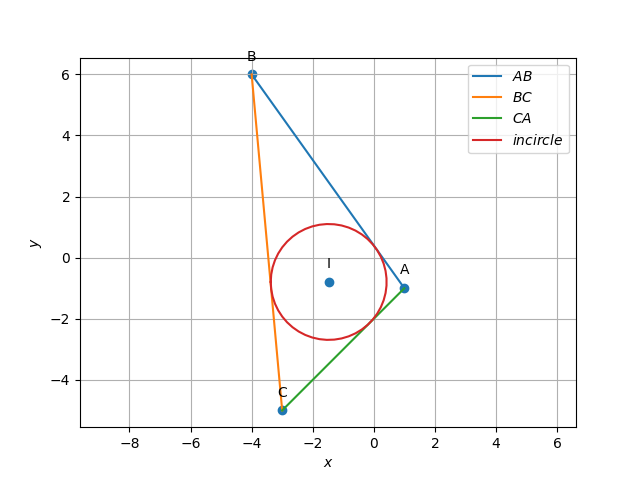
\includegraphics[width=\columnwidth]{solutions/1/5/7/figs/Diagram.png}
	\caption{Triangle with the incircle generated using python}
	\label{fig:Incircle}
\end{figure}

	The equation of the incircle is given as :

	\begin{align}
			\norm{\vec{x}-\vec{I}}^2 = r^2
	\end{align}

		\fi
\end{enumerate}

%
\chapter{Linear Equations}
\section{9}
\subsection{9.3.3}
\begin{enumerate}
\item In which quadrant or on which axis do each of the points(-2,4),(3,-1),(-1,0),(1,2) and (-3,-5) lie? Verify your answer by locating them on the Cartesian plane.
\item Plot the points $(x,y)$ given in the following table on the plane,choosing the suitable units of distance on the axes.
\begin{table}[h]
\begin{center}
\begin{tabular}{|c|c|c|c|c|c|}
\hline	
x & -2 & -1 & 0 & 1 & 3\\
\hline
y & 8 & 7 & -1.25 & 3 & -1\\
\hline
\end{tabular}
\caption{table of values}
\label{table:Table of values}
\end{center}
\end{table}
\end{enumerate}


\subsection{9.4.1}
\begin{enumerate}[label=\arabic*.,ref=\theenumi]
\item The cost of a notebook is twice the cost of a pen.Write a linear
equation in two variables to represent this statement.
(Take the Cost of a notebook to be $x$ and that of a pen to be
$y$).
\item Express the following linear equation in the form $ax+by+c=0$
and indicate the values of $a,b$ and $c$ in each case:
%\begin{enumerate}
\begin{enumerate}[label=(\roman*),ref=\theenumi]
\item $2x+3y=9.3\overline{5}$
\item $x-\frac{y}{5}-10=10$
\item $-2x+3y=6$
\item $ x=3y$
\item $2x=-5y$
\item $3x+2=0$
\item $y-2=0$
\item $5=2x$
\end{enumerate}
\end{enumerate}

\subsection{9.4.2}
\begin{enumerate}
\item Which one of the following options is true, and why?
 $y=3x+5$ has
\begin{enumerate}[label=(\roman*)]
\item a unique solution
\item only two solutions
\item infinitely many solutions
\end{enumerate}
\item Write four solutions for each of the following equations
\begin{enumerate}[label=(\roman*)]
\item $2x+y=7$
\item $\pi x+y=9$
\item $x=4y$
\end{enumerate}
\item Check which of the following are solutions of the equation $x-2y=4$ and which 
are not
\begin{enumerate}[label=(\roman*)]
\item ($0,2$)
\item ($2,0$)
\item ($4,0$)
\item ($\sqrt 2, 4\sqrt 2$)
\item ($1,1$)
\end{enumerate}
\item Find the value of $k$ if $x=2$, $y=1$ is a solution of the equation of the equation $2x+3y=4$
\end{enumerate}

\subsection{9.4.3}
\begin{enumerate}[label=\arabic*.,ref=\theenumi]
\item Draw the graph of each of the following linear equations in two variables:
\begin{enumerate}[label=(\roman*),ref=\theenumi]
\item $x+y=4$
\item $x-y=2$
\item $y=3x$
\item $3=2x+y$
\end{enumerate}
\item Give the equations of two lines passing through (2,14).How many more such lines are there and 
why?
\item If the point(3,4) lies on the graph of the equation $3y=ax+7$ find the value of a
\item The taxi fare in the city is as follows:for te first kilometre,the fare is \rupee~8 and for the 
subsquent distance is \rupee~5 per km.Taking the distance Covered as $x$ km and total fare as
\rupee~y.Write a linear equation for this information,and draw its graph.
\item From the choices given below,choose the equation whose graphs are given Fig 4.6 Fig 4.7
\\
For fig-4.6 
\begin{enumerate}[label=(\roman*)]
\item $y=x$
\item $x+y=0$
\item $y=2x$
\item $2+3y=7x$
\end{enumerate} 
For fig-4.7 
\begin{enumerate}[label=(\roman*)]
\item $y=x+2$
\item $y=x-2$
\item $y=-x+2$
\item $x+2y=6$
\end{enumerate}
\begin{figure}[ht]
\centering
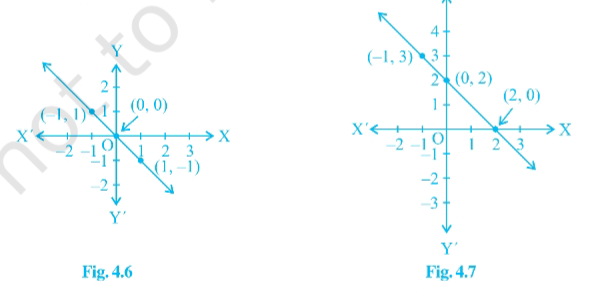
\includegraphics[width=\columnwidth]{chapters/9/figs/4.6-4.7.png}
\caption{Graph}
  \label{fig:4.6-4.7}
\end{figure}
\item If the work done by a body of a constant force is directly proportional 
to the distance travelled by the body,express this in the form of an equation
and draw the graph of the same by taking the varables and draw the graph of 
the same by taking the constant force as $5 units$.Also read from the graph the
work done when the distance travelled by the body is
\begin{enumerate}[label=(\roman*)]
\item $2$Units
\item $0$Unit
\end{enumerate}
\item Yamini and Fatima,two students of class IX of a school,together
 contributed \rupee~100 towards the prime minister's reief fund to help
 the earhquake victims.Write a linear equation which satisfies this data.
 (you may take their contributions  \rupee~x and \rupee~y.Draw the graph 
 of the same.
\item In Countries like USA and Canada temperature is measured in Celsius.
Here is a linear equation that converts Farenheit to celsius:
$F=\frac{9}{5}C+32$
\begin{enumerate}[label=(\roman*)]
\item Draw the graph of the linear equation above using Celsius for $x$
 axis and Farenheit for $y$ axis
\item If the temperature is $30\degree C$,what is the temperature in farenheight?
\item If the temperature is $95\degree F$,what is the temperature in celsius?
\item If the temperature is $0\degree C$.What is the temperature in Farenheit and if the temperature in celsius?
\item Is there a temperature Which is numerically same in both Farenheit and Celsius? If yes find it.
\end{enumerate}
\end{enumerate}

\section{10}
\subsection{Examples:-1-19 (10.3)}
\begin{enumerate}
\item Let us take the example given in Section 3.1. Akhila goes to a fair with \rupee~20 and wants to have rides on the Giant Wheel and play Hoopla. Represent this situation algebraically and graphically (geometrically).
\item Romila went to a stationary shop and purchased $2$ pencils and $3$ erasers for \rupee~9. Her friend Sonali saw the new variety of pencils and erasers with Romila, and she also bought $4$ pencils and $6$ erasers of the same kind for \rupee~18. Represent this situation algebraically and graphically.
\item Two rails are represented by the equations $x+2y-4=0$ and $2x+4y-12=0$. Represent this situation geometrically.
\item Check graphically whether the pair of equations.
\begin{align}
x+3y = 6 \\ \text{ and } 2x-3y = 12
\end{align}
is consistent. If so, Solve them graphically.
\item Graphically, find whether the following pair of equatons has no solution, unique solution or infinitely many solutions.
\begin{align}
5x-8y+1 = 0 \\ 3x-\frac{24}{5}y+\frac{3}{5} = 0
\end{align}
\item Champa went to a ``Sale" to purchase some pants and skirts. When her friends asked her how many of each she had boughtc she answered, ``The number of skirts is two less than twice the number of pants purchased. Also, the number of skirts is four less than four times the number of pants purchased". Help her friends to find how many pants and skirts Champa bought.
\item Solve the following pair of equations by substitution method:
\begin{align}
7x-15y = 2 \\  x+2y = 3
\end{align}
\item Solve Q.1 of Exercise 3.1 by the method of substitution.
\\ Aftab tells his daughter, ``Seven years ago, I was seven times as old as you were then. Also, three years from now, I shall be three times as old as you will be."  (Isn't this interesting ?) Represent this situation algebraically and graphically.
\item Let us consider Example 2 in Section $3.3$ i.e., the cost of 2 pencils and 3 erasers is \rupee~9 and the cost of 4 pencils and 6 erasers is \rupee~18. Find the cost of each pencil and each eraser.
\item Let us consider the Example $3$ of Section $3.2$. Will the rails cross each other? Two rails are represented by the equations $x+2y-4=0$ and $2x+4y-12=0$. Represent this situation geometrically.
\item The ratio of incomes of two persons is 9:7 and the ratio of their expenditures is $4:3$. If each of them manages to save \rupee~2000 per month, find their monthly incomes.
\item Use elimination method to find all possible solutions of the following pair of linear equations:-
\begin{align}
2x+3y = 8 \\ 4x+6y = 7
\end{align}
\item The sum of a two digit number and the number obtained by reversing the digits is $66$. If the digits of the number differ by 2, find the number. How many such numberes are there?
\item From a bus stand in Bangalore, if we buy $2$ tickets to Malleshwaram and $2$ tickets to yeshwanthpur the total cost is \rupee~74. Find the fare from the bus stand to Malleshwaram, and to Yeshwanthpur.
\item For which values $p$ does the pair of equations given below has unique solution.
\begin{align}
4x+py+8 = 0 \\ 2x+2y+2 = 0
\end{align}
\item For what values of $k$ will the following pair of linear equations have infinitely many solutions.
\begin{align}
kx+3y-(k-3) = 0 \\ 12x+ky-k = 0
\end{align}
\item Solve the pair of equations:
\begin{align}
\frac{2}{x}+\frac{3}{y}= 13 \\ \frac{5}{x}+\frac{4}{y} = -2
\end{align}
\item Solve the following pair of linear equations by reducing them to a pair of linear equations
\begin{align}
\frac{5}{x-1}+\frac{1}{y-2}= 2 \\ \frac{6}{x-1}-\frac{3}{y-2}= 1
\end{align}
\item A boat goes $30$ km upstream and $44$ km downstream in $10$ hours. In $13$ hours, it can go $40$ km upstream and $55$ km down-stream. Determine the speed of the stream and that of the boat in still water.
\end{enumerate}


  
 

\subsection{10.3.1}
\begin{enumerate}
\item Aftab tells his daughter, "Seven years ago, I was seven times as old as you were then. Also, $3$ years from now, I shall be $3$ times as old as  you will be. "(Isn't it interesting? Represent this situation algebraically and graphically.
\item The coach of a cricket team buys $3$ bats and $6$ balls for $Rs.3900$. Later, she buys another bat and $3$ more balls of the same kind for $Rs.3300$. Represent this situation algebraically and geometrically.
\item The cost of $2kg$ of apples and $1kg$ of grapes on a day was found to be $Rs.160$. After a month, the cost of $4kg$ of apples and $2kg$ of grapes is $Rs.300$. Represent this situation algebraically and geometrically.
\end{enumerate}

\subsection{10.3.2}
\begin{enumerate}
\item Form the pair of linear equations in the following problems and find their solutions graphically:
\begin{enumerate}[label=(\roman*)]
\item $10$ students of Class X took part in a Mathematics quiz. If the number of girls is $4$ more than the number of boys, find the number of boys and girls who took part in the quiz.
\item $5$ pencils and $7$ pens together cost $Rs. 50$ whereas $7$ pencils and $5$ pens together cost $Rs.46$. Find the cost of one pencil and that of one pen.
\end{enumerate}
\item On comparing the ratios $\frac{a_{1}}{a_2},\frac{b_1}{b_2} \text{and} \frac{c_1}{c_2}$, find out whether the lines representing the following pairs of linear equations intersect at a point, are parallel or coincident:
\begin{enumerate}[label=(\roman*)]
\item \begin{align}
	5x-4y+8=0\\ 
      	7x+6y-9=0
	\end{align}
\item \begin{align}
	9x+3y+12=0\\
	18x+6y+24=0
	\end{align}
\item \begin{align}
        6x-3y+10=0\\
	2x-y+9=0
	\end{align}
\end{enumerate}
\item On comparing the ratios $\frac{a_1}{a_2},\frac{b_1}{b_2} \text{and} \frac {c_1}{c_2}$, find out whether the following equations are consistent, or inconsistent:
\begin{enumerate}[label=(\roman*)]
	\item \begin{align}
       		3x+2y=5; \\
      		2x-3y=7
    	       \end{align} 
	\item \begin{align}
		2x-3y=8;\\
		4x-6y=9
		\end{align}
	\item \begin{align}
		\frac{3}{2}x+\frac{5}{3}y=7;\\
		9x-10y=14
		\end{align}
\item \begin{align}
		5x-3y=11;\\
		-10x+6y=-22
	\end{align}
\item \begin{align}
         \frac{4}{3}x+2y=8;\\
	  2x+3y=12
	\end{align}
\end{enumerate}
\item Which of the following pairs of linear equations are consistent/inconsistent? If consistent, obtain solution graphically:
\begin{enumerate}[label=(\roman*)]
\item \begin{align}
	x+y=5;\\
	2x+y=10
	\end{align}
\item \begin{align}
	x-y=8;\\
	3x-3y=16
	\end{align}
\item \begin{align}
 	2x+y-6=0;\\
 	4x-2y+4=0
	\end{align}
\item \begin{align}
	2x-2y-2=0;\\
	4x-4y-5=0
	\end{align}
\end{enumerate}
\item Half the perimeter of a rectangular garden,whose length is $4m$, more than its width,is $36m$. Find the dimensions of the garden.
\item Given the linear equation $2x+3y-8=0$, write another linear equation in two variables such that geometrical representation of the pair so formed is:
\begin{enumerate}[label=(\roman*)]
\item intersecting lines
\item parallel lines
\item coincident lines
\end{enumerate}
\item Draw the graphs of the equations $x-y+1=0$ and $3x+2y-12=0$. Determine the coordinates of the vertices of the triangle formed by these lines and the axis and shade the triangular region.
\end{enumerate}

\subsection{10.3.3}
\begin{enumerate}
\item Solve the following pair of linear equations by the substitution method.
\begin{enumerate}[label=(\roman*)]    
	\item
	\begin{align}
   	 x+y=14 \\x-y=4
	\end{align}
    	\item 
	\begin{align}
	s-t=3
	\end{align}
	\item
	\begin{align}
    	3x-y=3\\ 9x-3y=9
	\end{align}
	\begin{align}   	
 	0.2x+0.3y=1.3\\ 0.4x+0.5y=23
	\end{align}
	\item     
	\begin{align}
	\sqrt{2x}+\sqrt{3y}=0\\ \sqrt{3x}-\sqrt{8y}=0
	\end{align}
	\item
	\begin{align}
    	\frac{3x}{2}-\frac{5y}{2}=-2\\ \frac{x}{3}+\frac{y}{2}=\frac{13}{6}
    	\end{align}
	\end{enumerate}
\item Solve $2x+3y=11$ and $2x+4y=-24$ and hence find the value of $m$ for which $y=mx+3$
\item Form the pair of linear equations for the following problems and find their solutions by the substitution method
    \begin{enumerate}[label=(\Roman*)]
    \item The difference between two numbers is $26$ and one number is three times the other. Find them.
    \item The larger of two supplementary angles exceeds the smaller by $18$ degrees. Find them.
    \item The coach of a cricket team buys $7$ balls and $6$ balls for \rupee~3800. Later, she buys $3$ bats and $5$ balls for \rupee~1750. Find the cost of each bat and each ball.
    \item The taxi charges in a city consist of a fixed charge together with the charges for the distance covered. For a distance of $10$ km, the charge paid is \rupee~105 and for a distance of $15$ km, the charge paid is \rupee~155. What are the fixed charges and the charge per km? How much does a person have to pay for travelling a distance of 25 km ? 
    \item A fraction becomes $\frac{9}{11}$ if $2$ is added to both the numerator and the denominator. If $3$ is added to both the numerator and the denominator, it becomes $\frac{5}{6}$. Find the fraction.
    \item Five years hence, the age of Jacob will be three times that of his son. Five years ago, Jacob's age was seven times that of his son. What are their present ages?
    \end{enumerate}
\end{enumerate}

\subsection{10.3.4}
\begin{enumerate}
\item Solve the following pair of linear equations by the elimination method and the substitution method:
\begin{enumerate}[label=(\roman*)]
\item $x+y=5$ and $2x-3y=4$
\item $3x+4y=10$ and $ 2x-2y=2$
\item $3x-5y-4=0$ and $9x=2y+7$
\item $\frac{x}{2}+\frac{2y}{3}=-1$ and $x-\frac{y}{3}=0$
\end{enumerate}
\item Form the pair of linear equations in the following problem, and find their solutions(if they exist) by the elimination method:
\begin{enumerate}[label=(\roman*)]
\item If we add $1$ to the numerator and subtract $1$ from the denominator, a fraction reduces to $1$. It becomes $\frac{1}{2}$ if we only add $1$ to the denominator. What is the fraction?
\item Five years ago, Nuri was thrice as old as sonu. Ten years later, Nuri will be twice as old as sonu. How old are Nuri and sonu?
\item The Sum of the digits of a two-digit number is $9$. Also, nine times this number is twice the number obtained by reversing the order of the digits. Find the number.
\item Meena Went to a bank to withdraw \rupee~2000. She asked the cashier to give her \rupee~50 and \rupee~100 notes only. Meena got $25$ notes in all. Find how many notes \rupee~50 and \rupee~100 she received.
\item A lending library has a fixed charge for the first three days and an additional charge for each day thereafter. Sarita paid \rupee~27 for seven days, While susy paid \rupee~21 for the book she paid for five days. Find the fixed charge and the charge for each extra day.  
\end{enumerate}
\end{enumerate}

\subsection{10.3.5}
\begin{enumerate}
\item Which of the following pairs of linear equations has unique solution, no solution or infinitely many solutions.In case there is a unique solution,find it by using cross multiplication method:
  \begin{enumerate}[label=(\roman*)]
	\item \begin{align}
	x-3y-3=0\\
	3x-9y-2=0
        \end{align}
       \item \begin{align}
	2x+y=5\\
	3x+2y=8
	\end{align}
	\item \begin{align}
	3x-5y=20\\
	6x-10y=40
	\end{align}
	\item \begin{align}
	x-3y-7=0\\
	3x-3y-15=0
        \end{align}
 \end{enumerate}
\item 
  \begin{enumerate}[label=(\roman*)]
  \item For which values of $a$ and $b$ does the following pair of linear equations have an infinite number of solutions?
	\begin{align}
	2x+3y=7\\
	(a-b)x+(a-b)y=3a+b-2
	\end{align}
  \item For which value of $k$ will the following pair of linear equation have no solution?
	\begin{align}
	3x+y=1\\
	(2k-1)x+(k-1)y=2k+1
	\end{align}
   \end{enumerate}
\item Solve the following pair of linear equations by the substituions and cross multiplication method:
\begin{align}
8x+5y=9
\\ 3x+2y=4
\end{align}
\item Form the pair of linear equations in the following problems and find their solutions by any algebraic method:
\begin{enumerate}[label=(\roman*)]
\item A part of monthly hostel charges is fixed and the remaining depends on the number of days one has taken food in the mess. When a student $A$ takes food for $20$ days she has to pay Rs.$1000$ as hostel charges whereas a student $B$ who takes food for $26$ days, pays Rs.$1180$ as hostel charges. Find the fixed charges and the cost of food per day.
\item A fraction becomes $\frac{1}{3}$ when $1$ is subtracted from the numerator and it becomes $\frac{1}{4}$ when $8$ is added to the denominator. Find the fraction.
\item Yash scored $40$ marks in a test, getting $3$ marks for each right answer and losing $1$ mark for each wrong answer. Had $4$ marks been awarded for each correct answer and $2$ marks been deducted for each incorrect answer, then Yash would have scored $50$ marks. How many questions were there in the test?
\item Places $A$ and $B$ are $100km$ apart on a highway. One car starts from $A$ and another from $B$ at the same time. If the car travel in the same direction at different speeds, they meet in $5$hrs. If they travel towards each other, they meet in $1$hr. What are the speeds of the two cars?
\item The area of rectangle gets reduced by $9$ square units, if its length is reduced by $5$ units and breadth is increased by $3$ units. If we increase the length by $3$ units and the breadth by $2$ units, the area increases by $67$ square units. Find the dimensions of the rectangle.
\end{enumerate}
\end{enumerate}

\subsection{10.3.6}
\begin{enumerate}
\item Solve the following pair of equations by reducing them to a pair of linear equations:
\begin{enumerate}[label=(\roman*)]
\item
\begin{align}
\frac{1}{2x}+\frac{1}{3y}=2 \\ \frac{1}{3x}+\frac{1}{2y}=\frac{13}{6}
\end{align}
\item
\begin{align}
\frac{2}{\sqrt{x}}+\frac{3}{\sqrt{y}}=2\\
\frac{4}{\sqrt{x}}-\frac{9}{\sqrt{y}}=-1
\end{align}
\item
\begin{align}
\frac{4}{x}+3y=14\\ \frac{3}{x}-4y=23
\end{align}
\item
\begin{align}
\frac{5}{x-1}+\frac{1}{y-2}=2\\ \frac{6}{x-1}-\frac{3}{y-2}=1
\end{align}
\item
\begin{align}
\frac{7x-2y}{xy}=5\\ \frac{8x+7y}{xy}=15
\end{align}
\item
\begin{align}
6x+3y=6xy\\ 2x+4y=5xy
\end{align}
\item
\begin{align}
\frac{10}{x+y}+\frac{2}{x-y}=4\\ \frac{15}{x+y}-\frac{5}{x-y}=-2
\end{align}
\item
\begin{align}
\frac{1}{3x+y}+\frac{1}{3x-y}=\frac{3}{4}\\ \frac{1}{2(3x+y)}-\frac{1}{2(3x-y)}=\frac{-1}{8}
\end{align}
\end{enumerate}
\item Formulate the following problems as a pair of equations,and hence find their solutions:
\begin{enumerate}[label=(\roman*)]
\item Ritu can row downstream $20km$ in $2$ hours, and upstream $4km$ in $2$ hours. Find her speed of rowing in still water and the speed of the current.
\item $2$ women and $5$ men can together finish an embroidery work in $4$ days, while $3$ women and $6$ men can finish it in $3$ days. Find the time taken by $1$ women along to finish the work, and also that taken by $1$ men alone.
\item Roohi travels $300 km$ to her home partly by train and partly by bus. She takes $4$ hours if she travels $60km$ by train and the remaining by bus. If she travels $100km$ by train and the remaining by bus, she takes $10$ minutes longer. Find the speed of the train and the bus seperately.
\end{enumerate}
\end{enumerate}

\subsection{10.3.7}
\begin{enumerate}
\item The ages of two friends ani and Biju differ  by $3$  years. Ani's father dharam is twice as old as Ani and Biju is twice as old as sister cathy. The ages of cathy and dharam differ by $30$ years. Find the ages of Ani and Biju.
\item  One says, \textquotedblleft Give me a hundred, Friend !  I shall then become twice as rich as you \textquotedblright. The other \textquotedblleft  if you give me ten, i shall be six times as rich as you \textquotedblright.  Tell me What is the amount of their (respective) capital? [From the bijaganita of bhaskara II] 
\\ $[Hint: X+100=2(y-100), y+10=6(x-10)]$
\item A train Covered a certain distance at a uniform speed. If the train would have been 10 km/h faster, it would have taken $2$ hours less than the scheduled time. And, if the train were slower by 10 km/h; it would have taken $3$ hours more than the scheduled time. Find the distance covered by the train.
\item The students of a class are made to stand in rows. If 3 Students are extra in a row, there would be $1$ row less. If $3$ students are less in a row, there would be $2$ rows more. Find the number of stuents in the class.
\item In a $\triangle ABC, \angle C=3 \angle B=2(\angle A+\angle B)$. Find the three angles
\item Draw the graphs of the equations $5x-y=5$ and $3x-y=3$. Determine the Co-ordinates of the vertices of the triangle formed by these lines and the $y$ axis.
\item Solve the following pair of linear equations;
\begin{enumerate}
\item
\begin{align}
px+qy=p-q\\ qx-py=p+q
\end{align}
\item
\begin{align}                                                   
ax+by=c\\ bx+ay=1+c
\end{align}
\item 
\begin{align}
\frac {x}{a}-\frac{y}{b}=0\\ ax+by=a^2+b^2
\end{align}
\item
\begin{align}
(a-b)x+(a+b)y=a^2-2ab-b^2\\ (a+b)(x+y)=a^2+b^2
\end{align}
\item
\begin{align}
152x-378y=-74\\ -378x+152y=-604
\end{align}
\end{enumerate}
\item $ABCD$ is a cyclic quadrilateral [see \figref{fig:3.7}]. Find the angles of the cyclic quadrilateral.
\begin{figure}[ht]
\centering
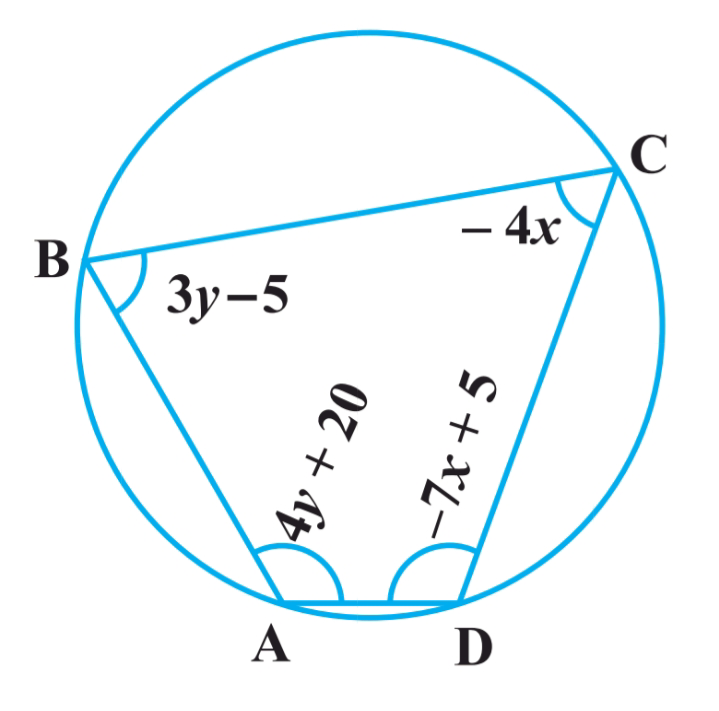
\includegraphics[width=\columnwidth]{chapters/10/figs/3.7.png}
\caption{3.7}
  \label{fig:3.7}
\end{figure}
\end{enumerate}


\chapter{Quadratic Equations}
\section{10}
\subsection{Examples:-1-18 (10.4)}                                               
\begin{enumerate}
\item Represent the following situation mathematically:
\begin{enumerate}[label=(\roman*)]
\item John and Jevanti together have $45$ marbles. Both of them lost $5$ marbles each, and the product of the number of marbles they now have is $124$. We would like to find out how many marbles they had to start with.
\item A cottage industry produces a certain number of toys a day. The cost of production of each toy (in Rupees) was found to be $55$ minus the number of toys produced in a day. On a particular day, the total cost of production was \rupee~750. We woud like to find out the number of toys produced on that day.
\end{enumerate}
\item Check whether the following are quadratic equations:
\begin{enumerate}[label=(\roman*)]
\item $(x-2)^2+1=2x-3$
\item $x(x+1)+8 = (x+2) (x-2)$
\item $x(2x+3) = X^2+1$
\item $(x+2)^3 = x^3-4$
\end{enumerate}
\item Find the roots of the equation $2x^2 -5x+3 = 0$  by factorisation.
\item Find the roots of the quadratic equation $6x^2 -x-2 = 0$.
\item Find the roots of the quadratic equation $3x^2 -2\sqrt6x+2 = 0$
\item Find the dimensions of the prayer hall discussed in Section $4.1$. A charity trust decides to build a prayer hall having a carpet area of 300 square metres with its length one metre more than twice its breath. What should be the length and breadth of the hall?
\item Solve the equation given in Example $3$ by the method of completing the square.
\item Find the roots of the equation $5x^2-6x-2 = 0$ by the method of completing the square.
\item Find the roots of $4x^2+3x+5 = 0$ by the method of completing the square.
\item Solve Q.2(i) of exercise $4.1$ by using the quadratic formula.
\begin{enumerate}[label=(\roman*)]
\item The area of a rectangle plot is $528 m^2$. The length of the plot (in metres) is one more than twice itsbreadth. We need to find the length and breadth of the plot.
\end{enumerate}
\item Find two consecutive odd positive integers, sum of whose squares is $290$.
\item A rectangular park is to be designed whose breadth is $3$ m less than its length. Its are is to be $4$ square metres than the area of a park that has already been made in the shape of a isoceles triangle with its base as  the breadth of the rectangular park and of altitude $12$ m (see \figref{fig:4.3}). Find its length and breadth.
\begin{figure}[h]
\centering
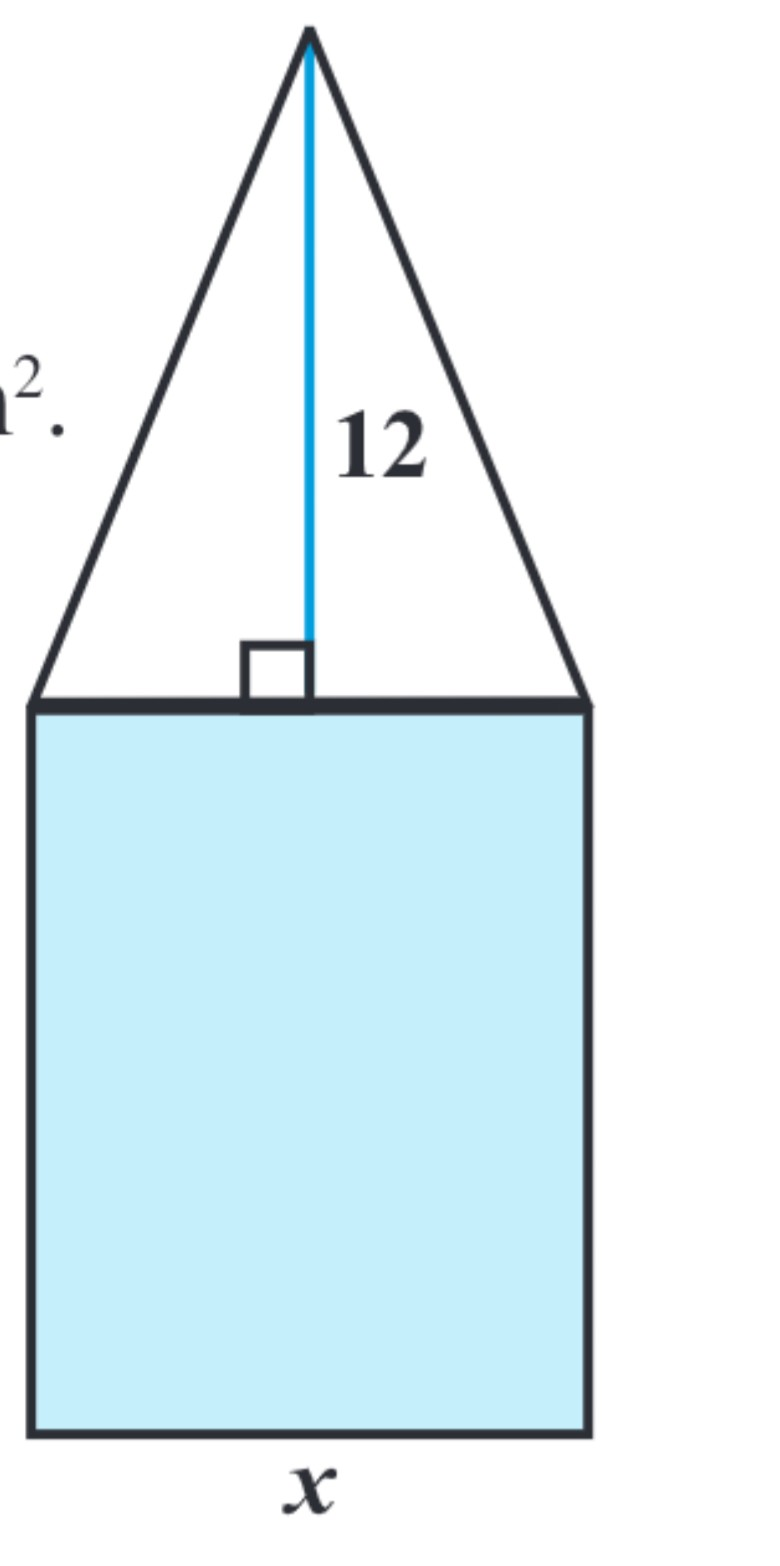
\includegraphics[width=\columnwidth]{chapters/10/figs/4.3.png}
\caption{4.3}
  \label{fig:4.3}
\end{figure}
\item Find the roots of the following quadratic equations, if they exist, using the quadratic formula.
\begin{enumerate}[label=(\roman*)]
\item $3x^2-5x+2 = 0$
\item $x^2+4x+5 = 0$
\item $2x^2-2\sqrt 2x+1 = 0$
\end{enumerate}
\item Find the roots of the following equations:
\begin{enumerate}[label=(\roman*)]
\item $x+\frac{1}{x} = 3,x\neq0$
\item $\frac{1}{x}-\frac{1}{x-2} = 3, x\neq 0,2$
\end{enumerate}
\item A motor boat whose speed is $18$ km/h in still water takes $1$ hour more to go $24$ km upstream than to return downstream to the same spot. Find the speed of the stream.
\item Find the discriminant of the quadratic equation $2x^2-4x+3 = 0$, and hence find the nature of its roots.
\item A pole has to be erected at a point on the boundary of a circular park of diameter $1.3$ metres in such a way that the difference of its distances from two diametrically opposite fixed gates A and B on the boundary is $7$ metres. Is it possible to do so? If yes, at what distances from the two gatees should the pole be erected ?
\item Find the discriminant of the equation $3x^2-2x+\frac{1}{3} = 0$ and hence find the nature of its roots. Find them, if they are real.
\end{enumerate}

\subsection{10.4.1}
\begin{enumerate}
\item Check whether the following are quadratic equations:
\begin{enumerate}[label=(\roman*)]
\item $(x+1)^2=2(x-3)$
\item $x^2-2x=(-2)(3-x)$
\item $(x-2)(x+1)=(x-1)(x+3)$
\item $(x-3)(2x-1)=x(x+5)$
\item $(2x-1)(x-3)=(x+5)(x-1)$
\item $x^2+3x+1=(x-2)^2$
\item $(x+2)^3=2x(x^2-1)$
\item $x^3-4x^2-x-1=(x-2)^3$
\end{enumerate}
\item Represent the folloing situations in form of quadratic equations:
\begin{enumerate}[label=(\roman*)]
\item The area of rectangulr plot is $528m^2$. The length of the plot (in metres) is one more than twice its breadth. We need to find the length and breadth of the plot.
\item The product of two consecutive positive integers is $306$. We need to find the integers.
\item Rohan's mother is $26$ years older than him. The product of their ages(in years) $3$ years from now will be $360$. We would like to find Rohan's present age.
\item A train travels a distance of $480km$ at a unifom speed. If the speed had been $8km/h$ less, then it would have taken $3 hours$ more to cover the same distance. We need to find the speed of the train.
\end{enumerate}
\end{enumerate}

\subsection{10.4.2}
\begin{enumerate}
\item  Find the roots of the following quadratic  equations by factorisation:
\begin{enumerate}[label=(\roman*)]
\item $x^2-3x-10=0$
\item $2x^2+x-6=0$
\item $ \sqrt 2x^2+7x+5 \sqrt 2=0$
\item $2x^2-x+\frac{1}{8}=0$
\item $100x^2-20x+1=0$
\end{enumerate}
\item Represent the following situations mathematically;
\begin{enumerate}[label=(\roman*)]
\item John and Jivanti together have $45$ marbles. Both of them lost $5$ marbles each, and the product of the number of marbles they have is $124$. We would like to find out how many marbles they had to start with.
\item A cottage industry produces a certain number of toys in a day. The cost of production of each toy (in rupees) was found to be $55$ minus the number of toys produced in a day. On a particular day, the total cost of production was \rupee~750. We would like to find out the number of toys produced on that day.
\end{enumerate}
\item Find two numbers whose sum is $27$ and product is $182$.
\item Find two consecutive  positive integers, sum of whose squares is $365$.
\item  The altitude of a right triangle is 7 cm less than its base. If the hypotenuse is 13 cm, find the other two sides.
\item A cottage industry produces a certain number of pottery articles in a day. It was observed on a particular day that the cost of production of each article (in rupees) was $3$ more than twice the number of articles produced on that day. If the total cost of production on that day was \rupee~90, find the number of articles produced and the cost of each article.
\end{enumerate}


\subsection{10.4.3}
\begin{enumerate}
\item Find the roots of the following quadratic equations, if they exist, by the method of completing the square:
\begin{enumerate}[label=(\roman*)]
\item
$2x^2-7x+3=0$
\item
$2x^2+x-4=0$
\item
$4x^2+4\sqrt 3x+3=0$
\item
$2x^2+x+4=0$
\end{enumerate}
\item Find the roots of the quadratic equations given in Q.1 above by applying the quadratic formula.
\item Find the roots of the following equations:
\begin{enumerate}[label=(\roman*)]
\item
\begin{align}
x-\frac{1}{x}=3, x\neq{0}
\end{align}
\item
\begin{align}
\frac{1}{x+4}-\frac{1}{x-7}=\frac{11}{30}, x\neq{-4,7}
\end{align}
\end{enumerate}
\item The sum of the reciprocals of Rehman's ages, (in years) 3 years ago and 5 years from now is $\frac{1}{3}$. Find his present age.
\item In a class test, the sum of shefali's  marks in Mathematics and english is $30$. Had she got $2$ marks more in Mathematics and $3$ marks less in English, the product of their marks would have been $210$. Find her marks in the two subjects. 
\item The diagonal of a rectangular field is $60$ metres more than the Shorter side. If the longer side is $30$ metres more than the shorter side, find the sides of the field.
\item The difference of squares of two numbers is $180$. The square of the smaller number is $8$ times the larger number. Find the two numbers.
\item A train travels $360$ km at a uniform speed. If the speed had been $5$ km/hr more, it would have taken $1$ hour less for the same journey. Find the speed of the train.
\item Two Water taps together can fill a tank in $9\frac{3}{8}$ hours.The tap of larger diameter takes $10$ hours.The tap of larger diameter takes $10$ hours less than the smaller one to fill the tank seperately. Find the time in which each tap can seperately fill the  tank.
\item An express train takes $1$ hour less than a passenger train to travel 132 km between mysore and bangalore (without taking into consideration the time they stop at intermediate statioons). If the average speed of the express train is 11 Km/h more than that of the passenger train, find the average speed of the two trains.
\item Sum of the areas of two square is $468m^2$. If the difference of their perimeter is 24m, find the sides of the two squares.  
\end{enumerate}


\subsection{10.4.4}
\begin{enumerate}
\item Find the nature of the roots of the following quadratic equations. If real roots exist, find them:
\begin{enumerate}[label=(\roman*)]
\item $2x^2-3x+5=0$
\item $3x^2-4 sqrt 3x+4=0$
\item $2x^2-6x+3=0$
\end{enumerate}
\item Find the values of k for each of the following quadratic equations, so that they hav equal roots:
\begin{enumerate}[label=(\roman*)]
\item $2x^2=kx-3=0$
\item $kx(x-2)+6=0$
\end{enumerate}
\item Is it possible to design a rectangular mango grove whose length is twice its breadth, and the area is  $800m^2$? If so, find its length and breadth.
\item Is the following situation possible? If so, determine their present ages.
\\ The sum of the ages of the two friends is 20 years. Four years ago, the product of their ages in years was $48$.
\item Is it possible to design a rectangular park of perimeter 80m and area of $400m^2$. If so, find its length and breadth.
\end{enumerate}


\chapter{Coordinate Geometry}
\section{10}
\subsection{Examples:-1-15 (10.7)}
\begin{enumerate}
\item Do the points $(3,2), (-2,-3)$ and $(2,3)$ form a triangle? If so, name the type of triangle formed.
\item Show that the points $(1,7),(4,2),(-1,-1)$ and $(-4,4)$ are the vertices of a square.
\item \figref{fig:7.6} shows the arrangement of desks in a classroom. Ashima, Bharti and Camella are seated at $A(3,1),B(6,4)$ and $C(8,6)$ respectively. Do you think they are seated in a line? Give reasons for your answer.
\begin{figure}[h]
\centering 
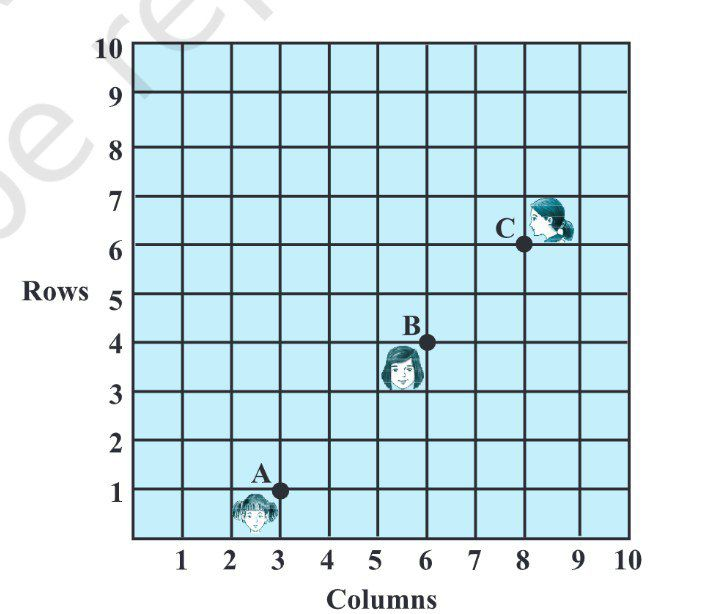
\includegraphics[width=\columnwidth]{chapters/10/figs/7.6.png}
\caption{7.6}
\label{fig:7.6}
\end{figure}
\item Find a relation between $x$ and $y$ such that the point $(x,y)$ is equidistant from the points $(7,1)$ and $(3,5)$.
\item Find a point on the Y-axis which is equidistant from the points $A(6,5)$ and $B(-4,3)$.
\item Find the coordinates of the point which divides the line segment joining the points $(4,-3)$ and $(8,5)$ in the ratio $3:1$ internally.
\item In what ratio does the point $(-4,6)$ divide the line segment joining the points $A(-6,0)$ and $B(3,-8)$?
\item Find the coordinates of the points of trisection (i.e. points dividing to three equal parts) of the line segment joining the points $A(2,-2)$ and $B(-7,4)$.
\item Find the ratio in which the Y-axis divides the line segment joining the points $(5,-6)$ and $(-1,-4)$. Also find the point of intersection.
\item If the points $A(6,1),B(8,2), C(9,4)$ and $D(p,3)$ are the vertices of a parallelogram, taken in order, find the value of $p$.
\item Find the area of the triangle whose vertices are $(1,-1), (-4,6)$ and $(-3,5)$.
\item Find the area of a triangle formed by the points $A(5,2), B(4,7)$ and $(7,-4)$.
\item Find the area of the triangle formed by the points $P(-1.5,3), Q(6,-2)$ and $R(-3,4)$.
\item Find the values of $k$ if the points $A(2,3), B(4,k)$ and $C(6,-3)$ are collinear.
\item If $A(-5,7), B(-4,-5), C(-1,-6)$ and $D(4,5)$ are the vertices of a quadrilateral, find the area of quadrilateral ABCD.
\end{enumerate}
 


\subsection{10.7.1}
\begin{enumerate}
\item Find the distance between the following pairs of points:
\begin{enumerate}[label=(\roman*)]
\item $(2,3), (4,1)$
\item $(-5,7), (-1,3)$
\item $(a,b), (-a,b)$
\end{enumerate}
\item Find the distance between the points $(0,0)$ and $(36,15)$. Can you now find the two town A and B discussed in section $7.2$.
\item Determine if the points $(1,5), (2,3)$ and $(-2,11)$ are collinear.
\item Check whether $(5,2), (6,4)$ and $(7,2)$ are the vertices of an isoceles triangle.
\item In a classroom, $4$ friends are seated at the points $A, B, C$ and $D$ as shown \figref{fig:7.8} in  Champa and chameli walk into the class and  after observing for a fwe minutes champa asks chameli, \textquotedblleft Don't you think ABCD is a square?\textquotedblright  Chameli disagrees Using distance formula, find which of them is correct.
	\begin{figure}[ht]
\centering
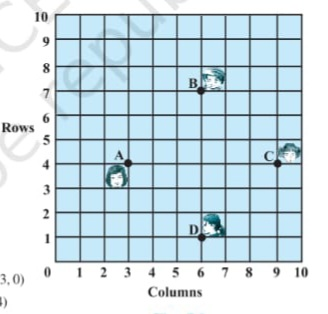
\includegraphics[width=\columnwidth]{chapters/10/figs/7.8.png}
\caption{7.8}
  \label{fig:7.8}
\end{figure}
\item Name the type of quadrilateral formed, if any, by the following points, and give reasons for your answer:
\begin{enumerate}[label=(\roman*)]
\item $(-1,2), (1,0), (-1,2), (3,0)$
\item $(-3,5), (3,1), (0,3), (-1,-4)$
\item $(4,5), (7,6), (4,3), (1,2)$
\end{enumerate}
\item Find the point on the $x$ axis which is equidistant from $(2,5)$ and $(2,9)$. 
\item Find the values of $y$ for which the distance between the points $P(2,-3)$ and $Q(10,y)$ is $10$ units.
\item $Q(0,1)$ is equidistant from $P(5,-3)$ and $R(x,6)$,find the values of $x$. Also find the distances $QR$ and $PR$.
\item Find a relation  between $x$ and $y$ such that $(x,y)$ is equidistant from the point $(3,6)$ and $(-3,4)$.
\end{enumerate}
	


\subsection{10.7.2}
\begin{enumerate}
\item Find the coordinates of the point which divides the join of $(-1,7)$ and $(4,-3)$ in the ratio 2:3.
\item Find the coordinates of the points of trisection of the line segment joining $(4,-1)$ and $(-2,3)$.
\item To conduct Sports Day activities, in your rectangular shaped school ground ABCD, lines have been drawn with chalk powder at a distance of 1m each. $100$ flower pots have been placed at a distance of 1m from each other along AD, as shown in \figref{fig:7.12}. Niharika runs $\frac {1}{4}th$ distance AD on the 2nd line and posts a green flag. Preet runs $\frac {1}{5}th$ the distance AD on the eighth line and posts a red flag. What is the distance between both the flags? If Rashmi has to post a blue flag exactly halfway between the line segment joining the two flags, where should she post her flag?
\begin{figure}[ht]
\centering
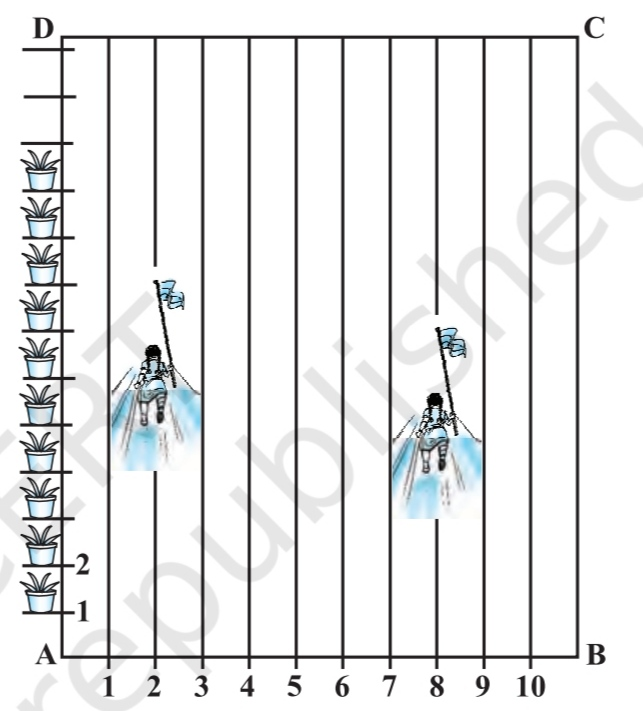
\includegraphics[width=\columnwidth]{chapters/10/figs/7.12.png}
\caption{7.12}
  \label{fig:7.12}
\end{figure}
\item Find the ratio in which the line segment joining the points $(-3,10)$ and $(6,-8)$ is divided by $(1,-6)$.
\item Find the ratio in which the line segment joining $A(1,-5)$ and $B(-4,5)$ is divided by the x-axis. Also find the coordinates of the point of division.
\item If $(1,2), (4,y), (x,6)$ and $(3,5)$ are the vertices of parallelogram taken in order, find x and y.
\item Find the coordinates of a point A, where AB is the diameter of a circle whose centre is $(2,-3)$ and B is $(1,4)$.
\item If A and B are $(-2,-2)$ and $(2,-4)$ respectively, find the coordinates of P such that AP= $\frac {3}{7}$ AB  and P lies on the line segment AB.
\item Find the coordinates of the points which divide the line segment joining A $(2,-2)$ and B $(2,8)$ into four equal parts.
\item Find the area of a rhombus if its vertices are $(3,0), (4,5), (1,-4)$ and $(-2,-1)$ taken in order.
\end{enumerate}

\subsection{10.7.3}
\begin{enumerate}
\item Find the area of the triangles whose vertices are:
\begin{enumerate}[label=(\roman*)]
\item $(2,3), (-1,0), (2,-4)$
\item $(-5,1), (3,-5), (5,2)$
\end{enumerate}
\item In each of the following value of 'K', for which the 
points are collinear.
\item Find the area of the triangle by joining the mid-points of the sides of the triangle whose vertices are $(0,1), (2,1)$ and $(0,3)$. Find the ratio of this area to the area of the given triangle.
\item Find the area of the quadrilateral whose vertices, taken in order, are $(-4,-2), (-3,-5), (3,-2)$ and $(2,3)$. 
\item You have studied in class IX (chapter 9, Example 3),that a median of a triangle divides in two triangles of equal areas. Verify this result for $\triangle ABC$ whose vertices are $A(4,-6), B(3,-2)$ and $C(5,2)$.
\end{enumerate}



\subsection{10.7.4}
\begin{enumerate}
\item Determine the ratio in which the line $2x+y-4=0$ divides the line segment joining the points $A(2,-2)$  and $B(3,7)$.
\item Find a relation between $x$ and $y$ if the points $(x,y), (1,2)$ and $(7,0)$ are collinear.
\item Find the centre of a circle passing through the points $(6,-6), (3,-7)$ and $(3,3)$.
\item The two opposite vertices of a square are $(-1,2)$ and $(3,2)$. Find the coordinates of the two other vertices.
\item The Class X students of a secondary school in Krishinagar have been allotted a rectangular plot of land for their gardening activity. Sapling of Gulmohar are planted on the boundary at a distance of 1m from each other. there is a triangular grassy lawn in the plot as shown in \figref{fig:7.14}. The students are to sow seeds of flowering plants on the remaining area of the plot.
\begin{enumerate}[label=(\roman*)]
\item Taking $A$ as origin, find the coordinates of the vertices of the triangle.
\item What will be tthe coordinates of the vertices of $\triangle PQR$ if $C$ is the origin Also calculate the areas of the triangles in these cases. What do you observe?
\end{enumerate}
\begin{figure}[ht]
\centering
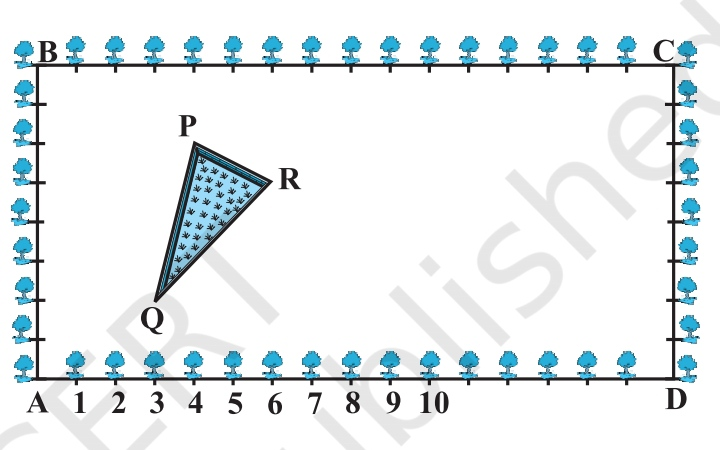
\includegraphics[width=\columnwidth]{chapters/10/figs/7.14.png}
\caption{7.14}
  \label{fig:7.14}
\end{figure}
\item The vertices of a $\triangle ABC$ are $A(4,6), B(1,5)$ and $C(7,2)$. A line is drawn to intersect sides $AB$ and $AC$ at $D$ and $E$ respectively, such that $\frac {AD}{AB}=\frac{AE}{AC}=\frac{1}{4}$. Calculate the area of the $\triangle AD$ and compare it with he area of $\triangle ABC$.
\item Let $A(4,2), B(6,5)$ and $C(1,4)$ be the vertices of $\triangle ABC$.
\begin{enumerate}[label=(\roman*)]
\item The median from $A$ meets $BC$ at $D$. Find the coordinates of the points $D$.
\item Find the coordinates of the point $P$ on $AD$ such that $AP:PD=2:1$.
\item Find the coordinates of points Q and R on medians $BE$ and $CF$ respectively such that $BQ:QE=2:1$ and $CR:RF=2:1$.
\item What do you observe?
\item If $A(x_1,y_1), B(x_2,y_2)$ and $C(x_3,y_3)$ are the vertices of $\triangle ABC$, find the coordinates of the triangle.
\end{enumerate}
\item  $ABCD$ is a rectangle formed by the points  $A(-1,-1), B(-1,4), C(5,4)$ and $D(5,-1)$. $P, Q, R$ and $S$ are the mid points of $AB, BC, CD$ and $DA$ respectively. Is the quadrilateral $PQRS$ a square? a rectangle? or a rhombus? Justify your answer.
\end{enumerate}

\chapter{Straight Lines}
\section{11}
\subsection{Examples:-1-25 (11.10)}
\begin{enumerate}
\item Find the slope of lines:
\begin{enumerate}
\item  Passing through the points $(3,-2)$ and $(-1,4)$
\item  Passing through the points $(3,-2)$ and $(7,-2)$
\item  passing through the points $(3,-2)$ and $(3,4)$	
\item  Making inclination of $60\degree$ with the positive direction of x-axis.
\end{enumerate}
\item If the angle between two lines is $\frac{\pi}{4}$ and slope of one of the lines is $\frac{1}{2}$, find the slope of the other line.
\item Line through the points $(-2,6)$ and $(4,8)$ is perpendicular to the line through the points $(8,12)$ and $(x,24)$. Find the value of $x$.
\item Three points $(h,k), Q(x_1,y_1)$ and $R(x_2,y_2)$ lie on a line. Show that $(h-x_1)(y_2-y_1)=(k-y_1)(x_2-x_1)$.
\item In \figref{fig:10.9}, time and distance graph of a linear motion is given. Two positions of line and distance are recorded as, when $T=0,D=2$ and when $T=3,D=8$. Use the concept of slope, find law of motion i.e, how distance depends upon time.
\begin{figure}[h]
\centering
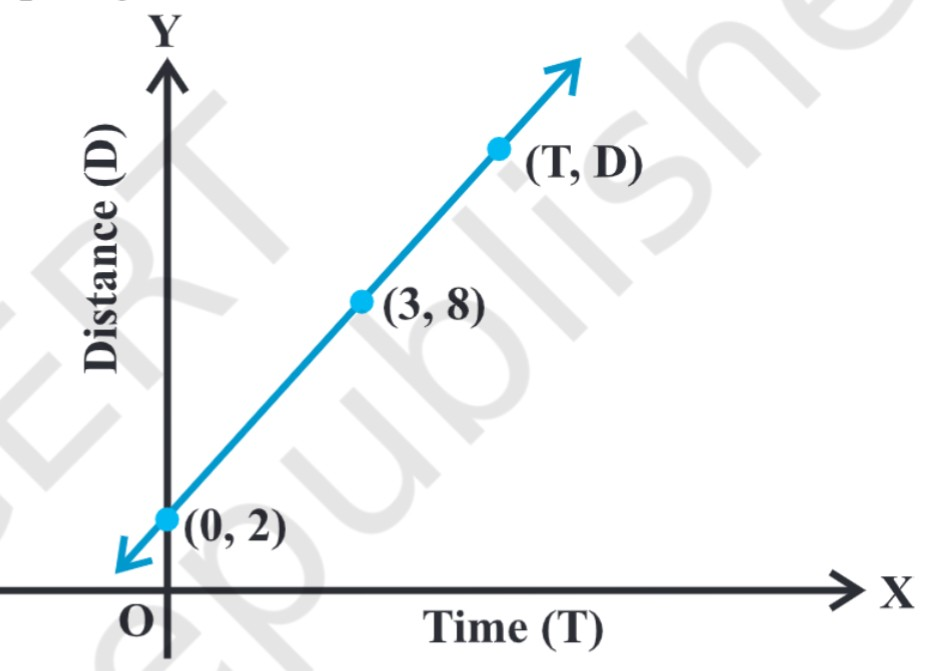
\includegraphics[width=\columnwidth]{chapters/11/figs/10.9.png}
\caption{10.9}
  \label{fig:10.9}
\end{figure}
\item Find the equations of the lines parallel to axes and passing through $(2,3)$.
\item Find the equation of the line through $(-2,3)$ with slope $-4$
\item Write the equation of the line through the points $(1,-1)$ and $(3,5)$.
\item Write the equation of the lines for which $\tan \theta=\frac{1}{2}$, where $\theta$ is the inclination of the line and
\begin{enumerate}[label=(\roman*)]
\item  y-intercepts is $\frac{-3}{2}$ 
\item  x-intercept is $4$.
\end{enumerate}
\item Find the equation of the lines which makes intercepts $-3$ and $2$ on the x- and y-axes respectively.
\item Find the equation of the line whose perpendicular distance from the origin is $4$ units and the angle which the normal makes with positive direction of x-axis is $15\degree$.
\item The Fahrenheit temperature $F$ and  absolute temperature $K$ satisfy a linear equation. Given that $K=273$ when $F=32$ and that $K=373$ when $F=212$. Express $K$ in terms of $F$ and find the value of $F$, when $K=0$.
\item Equation of a line is $3x-4y+10=0$, Find its
\begin{enumerate}[label=(\roman*)]
\item  Slope
\item  x and y-intercepts.
\end{enumerate}
\item Reduce the equation $\sqrt3x+y-8=0$ into normal form. Find the values of $p$ and $\omega$.
\item Find the angle between the lines $y-\sqrt 3x-5=0$ and $\sqrt 3y-x+6=0$.
\item Show that two lines $a_1x+b_1y+c_1=0$ and $a_2x+b_2y+c_2=0$ where $b_1b-2\neq 0$ are:
\begin{enumerate}
\item parallel if $\frac{a_1}{b_1}=\frac{a_2}{b_2}$ and 
\item Perpendicular if $a_1a_2-b_1b_2=0$.
\end {enumerate}
\item Find the equation of a line perpendicular to the line $x+2y+3=0$ and passing through the point $(1,-2)$.
\item Find the distance of the point $(3,-5)$ from the line $3x-4y-26=0$.
\item Find the distaance between the parallel lines $3x-4y+7=0$ and $3x-4y+5=0$.
\item If the lines $2x+y-3=0, 5x+ky-3=0$ and $3x-y-2=0$ are concurrent, find the value of $k$.
\item Find the distance of the line $4x-y-0$ from the point $p(4,1)$ measured along the line making an angle of $135\degree$ with the positive x-axis.
\item Assuming that straight lines work as the plane mirror for a point, find the image of the point $(1,2)$ in the line $x-3y+4=0$.
\item Show that the area of the triangle formed by the lines $y=m_1x+c_1, y=m_2x+c_2$ and $x=0$ is $\frac{c_1-c_2^2}{2\mydet{m_1-m_2}}$
\item A line is such that its segment between the lines $5x-y+4=0$ and $3x+4y-4=0$ is bisected at the point $(1,5)$. Obtain its equation.
\item Show that the path of a moving point such that its distances from two lines $3x-2y=5$ and $3x+2y=5$ are equal is a straight line.
\end{enumerate}
 

\subsection{11.10.1}

\begin{enumerate}
\item Draw a quadrilateral in the Cartesian plane, whose vertices are $(-4,5), (0,7), (5,-5)$ and $(-4,-2)$. Also, find its area.
\item The base of an equilateral triangle with side $2a$ lies along the y-axis such that the mid-point of the base is at the origin. Find vertices of the triangle.
\item Find the distance between $P(x_1,y_1),Q(x_2,y_2)$ when:
\begin{enumerate}[label=(\roman*)]
\item $PQ$ is parallel to the y-axis.
\item $PQ$ is parellel to the x-axis.
\end{enumerate}
\item Find the point x-axis, which is equidistant from the points $(7,6)$ and $(3,4)$.
\item Find the slope of a line, which passes through the origin, and the mid-point of the line segment joining the points $P(0,-4)$ and $B(8,0)$.
\item Without using the Pythagoras thorem, show that the points $(4,4), (3,5)$ and $(-1,-1)$ are the vertices of a right angled triangle.
\item Find the slope of the line, which makes an angle of 30° with the positive  direction of y-axis measured anticlockwise.
\item Find the value of $x$ for which the points $(x,-1), (2,1)$ and $(4,5)$ are collinear.
\item Without using distance formula, show that points $(-2,-1), (4,0), (3,3)$ and $(-3,2)$ are the vertices of the parallelogram.
\item Find the angle between the x-axis and the line joining the points $(3,-1)$ and $(4,-2)$.
\item The slope of a line is double of the slope of another line. If tangent of the angle between them is $\frac{!}{3}$, find the slopes of the lines.
\item A line passes through $(x_1,y_1)$ and $(h,k)$. If slope of the line is m, show that:
\item $k-y_1= m(h-x_1)$
\item If three points $(h,0), (a,b)$ and $(0,k)$ lie on a line, show that $\frac{a}{h}+\frac{b}{k}=1$.
\item Consider the following population and year graph  \figref{fig:10.10}, find the slope of the line $AB$ and using it, find what will be the population in the year $2010$?
\begin{figure}[ht]
\centering
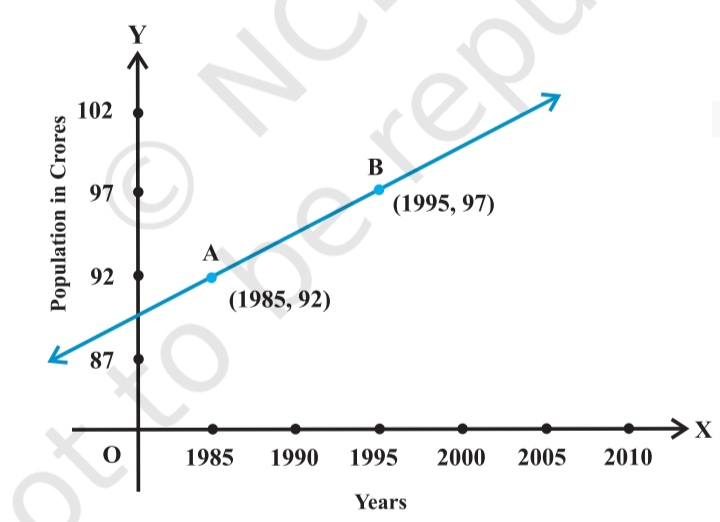
\includegraphics[width=\columnwidth]{chapters/11/figs/10.10.png}
\caption{10.10}
\label{fig:10.10}
\end{figure}
\end{enumerate}


\subsection{11.10.2}
 In excercises $1$ to $8$, find the equation of the line which satisfy  the given conditions:
\begin{enumerate}
\item Write the equations for $x$ and $y$ axes.
\item Passing through the point $(-4,3)$ with slope $\frac {1}{2}$.
\item Passing through $(0,0)$ with slope $m$.
\item Passing through $(2,\sqrt {3})$ and inclined with $x$ axis at an angle of $75\degree$.
\item Intersecting the $x$ axis at a distance of $3$ units to the left of the origin with slope $-2$.
\item Intersecting the $y$ axis at a distance of $2$ units above the origin and making an angle of $30°$ with positive direction of the $x$ axis.
\item Passing through the points $(-1,1)$ and $(2,-4)$.
\item Perpendicular distance from the origin is $5$ units and the angle made by the perpendicular with the positive $x$ axis is $30°$. 
\item The vertices of $\triangle PQR$ are $P(2,1), Q(-2,3)$ and $R(4,5)$. Find equation of the median through the vertex $R$.
\item Find the equation of the line passing through $(-3,5)$ and perpendicular to the line through the points $(2,5)$ and $(-3,6)$.
\item A line perpendicular to the line segment joining the points $(1,0)$  and $(2,3)$ divides it in the ratio $1:n$. Find the equation of the line.
\item Find the equation of the line that cuts off equal axes and passes through the point $(2,3)$.
\item Find equation of the line passing through the point $(2,2)$ and cutting off intercepts on the axes whose sum is $9$.
\item Find equation of the line through the point $(0,2)$ making an angle $\frac{2\pi}{3}$ with the positive $x$ axis. Also, find the equation of the parallel to it and crossing the $y$ axis at a distance of $2$ units below the origin.
\item The perpendicular from the origin to a line meets it at the point $(-2,9)$, find the equation of the line.
\item The length $L$ [in centimetre of a copper rod is a linear function of its celsius temperature $C$]. In an experiment, if $L=124.942$. When $C=20$  and $L=125.134$ When $C=110$, express $L$ in terms of $C$.
\item The owner of a milk store finds that, he can sell $980$ litres of milk each week at \rupee~14/litre and $1220$ litres of milk each week at \rupee~16/litre. Assuming a linear relationship between selling price and demand, how many litres could he sell weekly at \rupee~17/ litre?
\item $P(a,b)$ is the mid-point of a line segment between axes. Show that equation of the line is $\frac{x}{a}+\frac{y}{b}=2$
\item Point $R(h,k)$ divides a line segment betwween the axes in the ratio $1:2$. find equation of the line.
\item By Using the concept of equation of a line, prove that the three points (3,0), (-2,-2) and (8,2) are collinear.
\end{enumerate}


\subsection{11.10.3}
\begin{enumerate}
\item Reduce the following equations into slope-intercept form and find their slopes and the y-intercepts:
\begin{enumerate}[label=(\roman*)]
\item $x+7y=0$
\item $6x+3y-5=0$
\item $y=0$
\end{enumerate}
\item Reduce the following equations into intercept form and find their intercepts on the axes:
\begin{enumerate}[label=(\roman*)]
\item $3x+2y-12=0$
\item $4x-3y=6$
\item $3y+2=0$
\end{enumerate}
\item Reduce the folloeing equations into normal form. Find their perpendicular distances from the origin and angle between perpendicular and the positive x-axis:
\begin{enumerate}[label=(\roman*)]
\item $x-\sqrt3y+8=0$
\item $y-2=0$
\item $x-y=4$
\end{enumerate}
\item Find the distance of the point $(-1,1)$ from the line $12(x+6)=5(y-2)$.
\item Find the points on the x-axis, whose distances from the line $\frac{x}{3}+\frac{y}{4}=1$ are 4 units.
\item Find the distance between parallel lines:
\begin{enumerate}[label=(\roman*)]
           \item
 \begin{align}
        15x+8y-34=0 \text{ and } 15x+8y+31=0
              \end{align}
            \item
\begin{align}
        l(x+y)+p=0 \text{ and } l(x+y)-r=0
              \end{align}
\end{enumerate}
\item Find equation of the line parallel to the line $3x-4y+2=0$ and passing through the point $(-2,3)$.
\item Find equation of the line perpendicular to the line $x-7y+5=0$ and having $x$ intercept $3$.
\item Find angles between the lines $\sqrt3x+y=1$ and $x+\sqrt3y=1$.
\item The line through the points $(h,3)$ and $(4,1)$ intersects the line $7x-9y-19=0$ at right angle. Find the value of $h$.
\item Prove that the line through the point $(x,y)$ and parallel to the line $Ax+By+C=0$ is
\\ $A(x-x_1)+B(y-y_1)=0$.
\item Two lines passing through the point $(2,3)$ intersects each other at an angle at 60\degree. If the shape of one line is $2$, find equation of the other line.
\item Find the equation of the right bisector of the line segment joining the point $(3,4)$ and $(-1,2)$.
\item Find the coordinates of the foot of perpendicular4 from the point $(-1,3)$ to the line $3x+4y-16=0$
\item The perpendicular from the origin to the line $y=mx+c$ meets it at the point $(-1,2)$. Find the values of $m$ and $c$.
\item If $p$ and $q$ are the lengths of perpendiculars from the origin to the lines $x \cos \theta-y \sin \theta=k \cos 2 \theta$ and $x \sec \theta+y \cosec \theta=k$ respectively, prove that $p^2+4q^2=k^2$.
\item In the triangle $ABC$ ith vertices $A(2,3), B(4,-1)$ and $C(1,2)$, find the equation and length of altitude from the vertex $A$.
\item If $p$ is the length of perpendicular from the origin to the line whose intercepts on the axes are $a$  and $b$, then show that $\frac{1}{p^2}=\frac{1}{a^2}+\frac{1}{b^2}$.
\end{enumerate}

\subsection{11.10.4}
\begin{enumerate}
\item Find the values of $k$ for which the line $(k-3), x-(4-k^2) y+k^2-7k+6=0$ is
\begin{enumerate} 
\item Parallel to the $x$ axis.
\item Parallel to the $y$ axis.
\item Passing through the origin.
\end{enumerate}
\item Find the values of $\theta$ and $p$, if the equation $x \cos \theta + y \sin \theta = p$ is the normal form of the line $\sqrt 3x+y+2=0$.
\item Find the equations of the lines, which cut-off intercepts on the axes whose sum and product are $1$ and $-6$, respectively.
\item What are the points on the $y$ axis whose distance from the line $\frac{x}{3}+\frac{y}{4}=1$ is $4$ units.
\item Find perpendicular distance from the origin to the line joining the points $(\cos \theta, \sin \theta)$ and $(\cos \phi, \sin \phi)$.
\item Find the equation of the line parallel to $y$ axis and drawn through the point of intersection of the lines $x-7y+5=0$ and $3x+y=0$.
\item Find equation of a line drawn perpendicular to the line $\frac{x}{4}+\frac{y}{6}=1$ through the point, where it meets the $y$ axis.
\item Find the area of the triangle formed by the lines $y-x=0, x+y=0$ and $x-k=0$.
\item Find the value of $p$ so that the three lines $3x+y-2=0, px+2y-3=0$ and $2x-y-3=0, px+2y-3=0$ and $2x-y-3=0$ may intersect at one point.
\item If three lines when equation are $y=m_1x+c_1y=m_2x+c_2$ and $y=m_1x+c_1$ are concurrent, then show that $m_1 (c_2-c_3)+m_2(c_1-c_2)=0$
\item Find the equation of the lines through the point (3,2) which make an angle of $45\degree$ with the line $x-2y = 3$
\item Find the equation of the line passing through the point of intersection of the lines $4x+7y-3=0$ and $2x-3y+1=0$ that has equal interceptson the axes.
\item Show that the equation of the line passing through the origin and making an angle $\theta$ with the line $y=mx+c$ is $\frac{y}{x}=\frac{m \pm \tan \theta,}{1 \mp m\tan \theta,}$.
\item In what ratio, the line joining $(-1,1)$ and $(5,7)$ is divided by the line $x+y=4$?
\item Find the distance of the line $4x=7y+5=0$ from the point $(1,2)$ along the line $2x-y=0$.
\item Find the direction in which a straight line must be  drawn through the point $(-1,2)$ so that the point of intersection with the line $x+y=4$ may be at a distance of $3$ units from this point.
\item The hypothesis of a right angled triangle has its ends at the points $(1,3)$ and $(-4,1)$. Find an equation of the legs (perpendicular sides of the triangle.
\item Find the image of the point $(3,8)$ with respect to the line $x+3y=7$ assuming the line to be a plane mirror.
\item If the lines $y= 3x+1$ and $2y= x+3$ are equally inclined to the line $y= mx+4$. Find the value of $m$.
\item If sum of the perpendicular distance of a variable point $P(x,y)$ from the lines $x+y-5=0$ and $3x-2y+7=0$ is always $10$. Show that $P$ must move on a line.
\item Find equation of the line which is equidistant from parallel lines $9x+6y=-7$ and $3x+2y+6=0$.
\item A ray of the light passing through the point $(1,2)$ reflects on the $x$ axis at point $A$ and the reflected ray passes through the point $(5,3)$. Find the coordinates of $A$.
\item Prove that the product of the lengths of the perpendiculars drawn from the points $(\sqrt{a^2-b^2}, 0)$ and $(-\sqrt{a^2-b^2}, 0)$ to the line $\frac{x}{a} \cos \theta + \frac{y}{b} \sin \theta = 1$ is $b^2$
\item A person standing at the junction (crossing) of two straight paths represented by the equations $2x-3y+4=0$ and $3x+4y-5 = 0$ and $3x+4y-5= 0 $ wants to reach the path whose equation is $6x-7y+8=0$ in the least time. Find the equation of the path that he should follow.
\end{enumerate}

\chapter{Circles}
\section{11}
\subsection{11.11.1}
In each of the following exercise \ref{prob:1} to \ref{prob:5}, find the equation of the circle with:
\begin{enumerate}[label=\arabic*.,ref=\thesubsection.\theenumi]
\item centre $(0,2)$ and radius $2$ \label{prob:1}
\item centre $(-2,3)$ and radius $4$
\item centre $\frac({1}{2},\frac{1}{4})$ and radius $\frac {1}{!2}$
\item centre $(1,1)$ and radius $2$
\item centre $(-a,-b)$ and radius $\sqrt{a^2-b^2}$  \label{prob:5}
\end{enumerate}
In each of the following exercise \ref{prob:6} to \ref{prob:9}, find the centre and radius of the circles
\begin{enumerate}[resume]
\item $(x-5)^2+(y-3)^2=36$ \label{prob:6}
\item $x^2+y^2-4x-8y-45=0$
\item $x^2+y^2-8x+10y-12=0$
\item $2x^2+2y^2-x=0$ \label{prob:9}
\end{enumerate}
\begin{enumerate}[resume]
\item Find the equation of the circle passing through the points $(4,1)$ and $(6,5)$ and whose centre is on the line $4x+y=16$.
\item Find the equation of the circle passing through the points $(2,3)$ and $(-1,1)$ and whose centre is on the line $x-3y-11=0$.
\item Find the equation of the circle with radius 5 whose centre lies on x-axis and passes through the point $(2,3)$.
\item Find the equation of the circle passing through $(0,0)$ and making intercepts $a$ and $b$ on the coordinate axes.
\item Find the equation of a circle with centre $(2,2)$ and passes through the point $(4,5)$.
\item Does the point $(-2.5,3.5)$ lie inside, outside or on the circle $x^2+y^2=25$.
\end{enumerate}


\chapter{3D Geometry}
\section{11}
\subsection{Examples:-1-13 (11.12)}
\begin{enumerate}
\item In \figref{fig:12.3}, if $P$ is $(2,4,5)$, find the coordinates of $F$.
\begin{figure}[h]
\centering
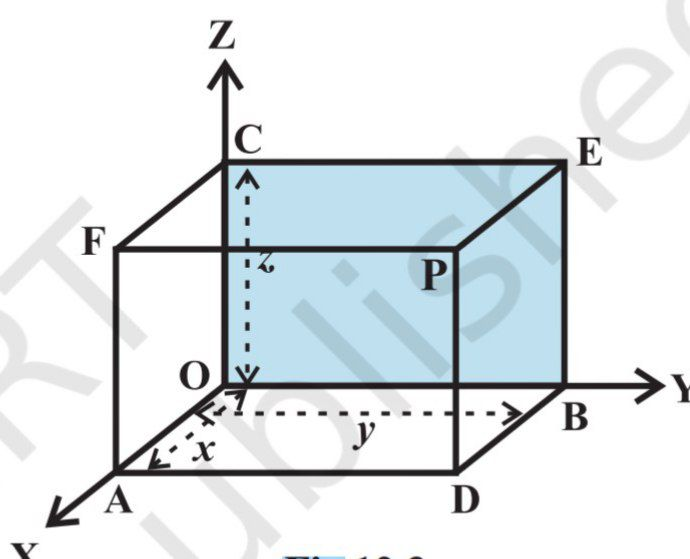
\includegraphics[width=\columnwidth]{chapters/11/figs/12.3.png}
\caption{12.3}
\label{fig:12.3}
\end{figure}
\item Find the octant in which the points $(-3,1,2)$ and $(-3,1,-2)$ lie.
\item Find the distance between the origin $O$ and any point $Q(x_2,y_2,z_2)$.
\item Show that the points $P(-2,3,5), Q(1,2,3)$ and $R(7,0,-1)$ are collinear. 
\item Are the points $A(3,6,9), B(10,20,30)$ and $C(24,-41,5)$ the vertices of a right angled triangle?
\item Find the equation of set of points $P$ such that $PA^2+PB^2=2k^2$, where $A$ and $B$ are the points $(3,4,5)$ and $(-1,3,-7)$, respectively.
\item Find the coordinates of the point which divides the line segment joining the points $(1,-2,3)$ and $(3,4,-5)$ in the ratio $2:3$
\begin{enumerate}[label=(\roman*)]
\item internally, and
\item externally
\end{enumerate}
\item Using section formula, prove that the three points $(-4,6,10), (2,4,6)$ and $(14,0,-2)$ are collinear.
\item Find the coordinates of the centroid of the triangle whose vertices are $(x_1,y_1,z_1), (x_2,y_2,z_2)$ and $(x_3,y_3,z_3)$.
\item Find the ratio in which the line segment joining the points $(4,8,10)$ and $(6,10,-8)$ is divided by the $YZ$- plane.
\item Show that the points $A(1,2,3), B(-1,-2,-1), C(2,3,2)$ and $D(4,7,6)$ are the vertices of a parallelogram $ABCD$, but it is not a rectangle.
\item Find the equation of the set of the points $P$ such that its distances from the points $A(3,4,-5)$ and $B(-2,1,4)$ are equal.
\item The centroid of a triangle $ABC$ is at the point $(1,1,1)$. If the coordinates of $A$ and $B$ are $(3,-5,7)$ and $(-1,7,-6)$, respectively find the coordinates of the point $C$.
\end{enumerate}


\subsection{11.12.1}
\begin{enumerate}
\item $A$ points is on the axis. What are its $y$ coordinate and $z$ coordinates?
\item $A$ point  in the $XZ$-plane. What can you say about its $y$ coordinates?
\item Name the octants in which the  following points  lie:
\begin{align}
(1,2,3), (4,-2,3), (4,-2,-5), (4,2,-5), (-4,2,-5), (-4,2,-5), (-3,-1,6), (-2,-4,-7)
\end{align}
\item Fill in the blanks:- 
\begin{enumerate}[label=(\roman*)]
\item The $x$ axis and $y$ axis taken together determine a plane known as \rule{1cm}{0.15mm} .
\item The coordinates of points in the $XY$. plane are of the form \rule{1cm}{0.15mm}.
\item Coordinate plane divide the space into  \rule{1cm}{0.15mm} octants.
\end{enumerate}
\end{enumerate}


\subsection{11.12.2}
\begin{enumerate}
\item Find the distance between the following pairs of points:
\begin{enumerate}[label=(\roman*)]
\item $(2,3,5)$ and $(4,3,1)$
\item $(-3,7,2)$ and $(2,4,-1)$
\item $(-1,3,-4)$ and $(1,-3,4)$
\item $(2,-1,3)$ and $(-2,1,3)$
\end{enumerate}
\item Show that the points $(-2,3,5), (1,2,3)$ and $(7,0,-1)$ are collinear.
\item Verify the following:
\begin{enumerate}[label=(\roman*)]
\item $(0,7,-10), (1,6,-6)$ and $(4,9,-6)$ are the vertices of an isoceles triangle.
\item $(0,7,10), (-1,6,6)$ and $(-4,9,6)$ are the vertices of a right angled triangle.
\item $(-1,2,1), (1,-2,5), (4,-7,8)$ and $(2,-3,4)$ are the vertices of a parallelogram.
\end{enumerate}
\item Find the equation of the set of points which are equidistant from the points $(1,2,3)$ and $(3,2,-1)$.
\item Find the equation of the set of points $P$, the sum of whose distances from $A(4,0,0)$ and $B(-4,0,0)$ is equal to $10$.
\end{enumerate}

\subsection{11.12.3}
\begin{enumerate}
\item Find the coordinates of the point which divides the line segment joining the points which divides the line segment joining  the points $(-2,3,5)$ and $(1,-4,6)$ in the ratio 
\begin{enumerate}
\item $2:3$ internally,
\item $2:3$ externally
\end{enumerate}
\item Given that $P(3,2,-4), Q(5,4,-6)$ and $R(9,8,-10)$ are Collinear. Find the ratio in which $Q$ divides $PR$.
\item Find the ratio in which the $yz$ plane divides the line segment formed by joining the points $(-2,4,7)$ and $(3,-5,8)$.
\item Using section formula, show that the points $A(2,-3,4), B(-1,2,1)$ and $C(0,\frac{1}{3},2)$ are collinear.
\item Find the coordinates of the points which triset the line segment joining the points $P(4,2,-6)$ and $Q(10,-16,6)$.
\end{enumerate}


\subsection{11.12.4}
\begin{enumerate}
\item Three vertices of a parallelogram $ABCD$ are $A(3,-1,2), B(1,-2,4)$ and $C(-1,1,2)$. Find the coordinates of the fourth vertex.
\item Find the lengths of the medians of the triangle with vertice $A(0,0,6), B(0,4,0)$ and $(6,0,0)$.
\item If the origin is the centroid of the triangle $PQR$ with vertices $P(2a,2,6), Q(-4,3b,-10)$ and $R(8,14,2c)$, then find the values of $a, b$ and $c$.
\item Find the coordinates of a point on y-axis which are at a distance of $5\sqrt2$ from the point $P(3,-2,5)$.
\item A point $R$ with x-coordinate $4$ lies on the line segment joining the points $P(2,-3,4)$ and $Q(,0,10)$. Find the coordinates of the point $R$.
\item If $A$ and $B$ be the points $(3,4,5)$ and $(-1,3,-7)$ respectively, find the equation of the set of the points $P$ such that $PA^2+PB^2=K^2$ where $K$ is a constant.
\end{enumerate}

\chapter{Matrices}
\section{12}
\subsection{Examples:-1-28 (12.3)}
\begin{enumerate}
\item Consider the following information regarding the number of men ad women workers in three factories I, II and III 
\begin{table}[ht!]
\centering
\begin{tabular}{|c|c|c|}
\hline
 & Men Workers & Women Workers\\
\hline
I &30&27\\
\hline
II  &25&31\\
\hline
III &27&26\\
\hline
\end{tabular}
\caption{}
\end{table}\\
Represent the above information in the form of a $3\times 2$ matrix. What does the entry in the third row and second column represent $?$
\item If a matrix has $8$ elements, what are the possible orders it can have ?
\item Construct a $3\times 2$ matrix whose elements are given by $a_{ij}= \frac{1}{2}\abs{1-3j}$
\item If $\myvec{x+3&z+4&2y-7\\-6&a-1&0\\b-3&-21&0}=\myvec{0&6&3y-2\\-6&-3&2c+2\\2b+4&-21&0}$. Find the values of $a,b,c,x,y$ and $z$. 
\item Find the values of $a, b, c$ and $d$ from the following equation :
\begin{align} 
\myvec{2a+b&a-2b\\5c-d&4c+d} = \myvec{4&-3\\11&24} 
\end{align}
\item Given $A=\myvec{\sqrt{3}&1&-1\\2&3&0}$ and $B=\myvec{2&\sqrt{5}&1\\-2&3&\frac{1}{2}}$, find $A+B$.
\item If $A=\myvec{1&2&3\\2&3&1}$ and $B=\myvec{3&-1&3\\-1&0&2}$, then find $2A-B$.
\item If $A=\myvec{8&0\\ 4&-2\\3&6}$ and $B=\myvec{2&-2\\4&2\\-5&1}$ then find that $X$, such that $2A+3X=5B$
\item Find $X$ and $Y$, if $X+Y=\myvec{5&2\\0&9}$ and $X-Y=\myvec{3&6\\0&-1}$
\item Find the values of $x$ and $y$ from the following equations:
\begin{align} 2 \myvec{x&5\\7&y-3}+\myvec{3&-4\\1&2}=\myvec{7&6\\15&14} \end{align}
\item Two farmers Ramkishan and Gurucharan Singh cultivate only three varities of rice namely Basmati, Permal and Naura. The sale (in Rupees) of these three varities of rice by both the farmers in the month of September and October are given by the following matrices $A$ and $B$.
 \\ September Sales (in Rupees)
\begin{align}
A=\myvec{ \text{Basmati} & \text{Permal} & \text{Naura}\\ 10000&20000&30000\\50000&30000&10000} \begin{array}{c}\text{Ramkishan}\\ \text{Gurucharan Singh}\end{array}
\end{align}
  October Sales (in Rupees)
\begin{align}
B=\myvec{\text{Basmati}& \text{Permal} &\text{Naura}\\5000&10000&6000\\20000&10000&10000}\begin{array}{c}\text{Ramakishan} \\ \text{Gurucharan Singh}\end{array}
\end{align}
\begin{enumerate}[label=(\roman*)]
\item Find the combined sales in Sepember and October for each farmer in each variety.
\item Find the decrease in sales from September to October.
\item If both farmers receive $2\%$  profit on gross sales, compute the profit for each farmer and for each variety sold in October.
\end{enumerate}
\item Find $AB$, if $A=\myvec{6&9\\2&3}$ and $B=\myvec{2&6&0\\7&9&8}$.
\item If $A=\myvec{1&-2&-3\\ -4&2&5}$ and $B=\myvec{2&3\\4&5\\2&1}$, then find $AB, BA$. Show that $AB\neq BA$.
\item If $A=\myvec{1&0\\0&-1}$ and $B=\myvec{0&1\\1&0}$, then $AB=\myvec{0&1\\-1&0}$ and $BA=\myvec{0&-1\\1&0}$ clearly $AB\neq BA$. Thus matrix multiplication is not commutative.
\item Find $AB$, if $A=\myvec{0&-1\\0&2}$ and $B=\myvec{3&5\\0&0}$.
\item If $A=\myvec{1&1&-1\\2&0&3\\3&-1&2}, B=\myvec{1&2\\0&2\\-1&4}$ and $C=\myvec{1&2&3&-4\\2&0&-2&1}$ find $A(BC), (AB)C$ and show that $(AB)C = A(BC)$.
\item If $A=\myvec{0&6&7\\-6&0&8\\7&-8&0}, B=\myvec{0&1&1\\1&0&2\\1&2&0}, C=\myvec{3\\-2\\3}$ Calculate $AC,BC$ and $(A+B)C$. Also,  verify that $(A+B)C=AC+BC$.
\item If $A=\myvec{1&2&3\\3&-2&1\\4&2&1}$, then show that $A^3-23A-40I=0$.
\item In a legislative assembly election, a political group hired a public relations firm to promote its candidate in three ways: telephone, housecalls and letters. The cost per contact (in paise) is given in matrix $A$ as \\ cost per contact  
\begin{align} A=\myvec{40\\100\\50}\begin{array}{c} \text{Telephone}\\ \text{Housecall}\\ \text{Letter}\end{array}\end{align}.
\\ The number of contacts of each type made in two cities $X$ and $Y$ is given by 
\begin{align} B=\myvec{\text{Telephone}&\text{Housecall}&\text{Letter} \\ 1000&500&5000\\3000&1000&10000}\begin {array}{c} X\\Y\end{array}\end{align}. 
\\ Find the total amount spent by the group in the two cities $X$ and $Y$.
\item If $A=\myvec{3&\sqrt3&2\\4&2&0}$ and $B=\myvec{2&-1&2\\1&2&4}$, verify that 
\begin{enumerate}
\item $(A^{\prime})^{\prime}=A$
\item $(A+B)^{\prime}=A^{\prime}+B^{\prime}$
\item $(kB)^{\prime}=kB^{\prime}$, where $k$ is any constant.
\end{enumerate}
\item If $A=\myvec{-2\\4\\5}, B=\myvec{1&3&-6}$, verify that $(AB)^{\prime}=B^{\prime}A^{\prime}$.
\item Express the matrix $B=\myvec{2&-2&-4\\-1&3&4\\1&-2&-3}$ as the sum of symmetric and a skew symmetric matrix.
\item By using elementary operations, find the inverse of the matrix $A=\myvec{1&2\\2&1}$.
\item Obtain the inverse of the following matrix using elementary operations. 
\begin{align}A=\myvec{0&1&2\\1&2&3\\3&1&1} \end{align}.
\item Find $P^{-1}$, if it exists, given $P=\myvec{10&-2\\-5&1}$.
\item If $A=\myvec{\cos \theta& \sin \theta\\ -\sin \theta&\cos\theta}$, then prove that $A^n=\myvec{\cos n\theta&\sin n\theta\\ -\sin n\theta&\cos n\theta}, n\in N$.
\item If $A$ and $B$ are symmetric matrices of the same order, then show that $AB$ is symmetric if and only if $A$ and $B$ commute, that is $AB=BA$.
\item Let $A=\myvec{2&-1\\3&4}, B=\myvec{5&2\\7&4}, C=\myvec{2&5\\3&8}$. Find a matrix $D$ such that $CD-AB=0$.
\end{enumerate}

\subsection{12.3.1}
\begin{enumerate}
\item In the matrix $A=\myvec
{2 & 5 & 19 & -7\\
25 & -2 & \frac{5}{2} & 12\\
\sqrt 3 & 1 & -5 & 17}$, write:
\begin{enumerate}[label=(\roman*)]
\item The order of the matrix
\item The number of elements
\item Write the elements $a_{13}, a_{21}, a_{33}, a_{24}, a_{23}$
\end{enumerate}
\item If a matrix has $24$ elements, what are the possible order it can have? What if, it has $13$ elements?
\item If a matrix has $18$ elements, what are the possible orders it can have? What, if it has $5$ elements?
\item Construct a $2\times 2$ matrix, $A=[a_{ij}]$, whose elements are given by:
\begin{enumerate}[label=(\roman*)]
\item $[a_{ij}]=\frac{(i+j)^2}{2}$
\item $[a_{ij}]=\frac{i}{j}$
\item $[a_{ij}]=\frac{(i+2j)^2}{2}$
\end{enumerate}
\item Construct a $3\times 4$ matrix, whose elements are given by:
\begin{enumerate}[label=(\roman*)]
\item $[a_{ij}]=\frac{1}{2}\abs{-3i+j}$
\item $[a_{ij}]=2i-j$
\end{enumerate}
\item Find the values of $x, y$ and $z$ from the following equations:
\begin{enumerate}[label=(\roman*)]
\item $\myvec
{4 & 3 \\ x & 5}= 
\myvec{y & z \\ 1 & 5}$
\item $\myvec
{x+y & 2 \\ 5+z & xy}=
\myvec{ 6 &  2 \\  5  & 8}$
\item $\myvec
{x+y+z \\ x+z \\ y+z }=
\myvec{9 \\ 5 \\  7}$
\end{enumerate}
\item Find the value of $a, b, c$ and $d$ from the equation:
\begin{align} \myvec 
{a-b & 2a-c \\ 2a-b &  3c+d } = 
\myvec{-1 & 5 \\ 0 & 13} \end{align}
\item $A=[a_{ij}]_{m\times n}$ is a square matrix, if:
\begin{enumerate}
\item $m \le n$
\item $m \ge n$
\item $m=n$
\item None of these
\end{enumerate}
\item Which of the given values of $x$ and $y$ make the following pair of matrices equal:
\begin{align} \myvec
{3x+7 & 5 \\ y+1 & 2-3x}, 
\myvec{0 & y-2 \\ 8 & 4}\end{align}
\begin{enumerate}
\item $x=\frac{1}{3}, y=7$
\item Not possible to find 
\item $y=7, x=\frac{2}{3}$
\item $x=\frac{1}{3}, y=\frac{2}{3}$
\end{enumerate}
\item The number of all possible matrices of order $3\times 3$ with each entry $0$ or $1$ is:
\begin{enumerate}
\item $27$
\item $81$
\item $18$
\item $512$
\end{enumerate}
\end{enumerate}

 






\subsection{12.3.2}
\begin{enumerate}
\item Let $A= \myvec
 {2 & 4 \\ 3 & 2}, B=\myvec
 {1 & 3 \\ -2 & 5} , C=\myvec
{-2 & 5 \\ 3 & 4}$.
 Find each of the following:
\begin{enumerate}[label=(\roman*)]
\item $A+B$
\item $A-B$
\item $3A-C$
\item $AB$
\item $BA$
\end{enumerate}
\item Compute the following:
\begin{enumerate}[label=(\roman*)]
\item $\myvec  
{a & b \\ -b & a}+
\myvec{a & b \\ -b & a}$
\item $\myvec
{a^2+b^2 & b^2+c^2 \\ a^2+c^2 & a^2+b^2}+\myvec
{2ab & 2ac \\ -2ac & -2ab}$
\item $\myvec
{-1 & 4 & -6 \\ 8 & 5 & 16 \\ 2 & 8 & 5}+\myvec
{12 & 7 & 6 \\ 8 & 0 & 5 \\ 3 & 2 & 4}$
\item $\myvec
{\cos^2x & \sin^2x \\ \sin^2x & \cos^2x}+ \myvec{\sin^2x & \cos^2x \\ \cos^2x & \sin^2x}$
\end{enumerate}
\item Compute the following products:
\begin{enumerate}[label=(\roman*)]
\item $\myvec
{a & b  \\ b & -a} \myvec
{a & -b \\ b & a}$
\item $\myvec
{1 \\ 2 \\ 3 } \myvec
{2 & 3 & 4}$
\item $\myvec
{2 & 3 & 4 \\ 3 & 4 & 5 \\ 4 & 5 & 6 } \myvec
{1 & -3 & 5 \\ 0 & 2 & 4 \\ 5 & 0 & 5}$
\item  $\myvec
{2 & 1 \\ 3 & 2 \\ -1 & 1}\myvec
{1 & 0 & 1 \\ -1 & 2 & 1}$
\item $\myvec
{3 & -1 & 3 \\ 1 & 0 & 2 } \myvec
{2 & -3 \\ 1 & 0 \\ 3 & 1}$
\end{enumerate}
\item If $A=\myvec
{1 & 2 & -3 \\ 5 & 0 & 2 \\ 1 & -1 & 1}, B=\myvec
{3 & -1 & 2 \\ 4 & 2 & 5 \\ 2 & 0 & 3}$ and $C=\myvec
{4 & 1 & 2 \\ 0 & 3 & 2 \\ 1 & -2 & 3}$, then compute $(A+B)$ and $(B+C)$. Also, verify
that $A+(B-C)=(A+B)-C$.
\item If $A=\myvec
{\frac{2}{3} & 1 & \frac{5}{3} \\ \frac{1}{3} & \frac{2}{3} & \frac{4}{3} \\ \frac{7}{3}& 2 & \frac{2}{3}}$  and $B= \myvec
{\frac{2}{5} & \frac{3}{5} & 1 \\ \frac{1}{5} & \frac{2}{5} & \frac{4}{5} \\ \frac{7}{5} & \frac{6}{5} & \frac{2}{5}}$, then compute $3A-5B$.
\item Simplify $\cos \theta \myvec {\cos \theta & \sin \theta \\ -\sin \theta & \cos \theta} + \sin \theta \myvec{\sin \theta & -\cos \theta \\ \cos \theta & \sin \theta}$.
\item Find $X$ and $Y$, if:
\begin{enumerate}[label=(\roman*)]
\item $X+Y= \myvec
{7 & 0 \\ 2 & 5}$  and $X-Y=\myvec
{3 & 0 \\ 0 & 4}$.
\item $2X+3Y=\myvec
{2 & 3 \\ 4 & 0}$ and $3X+2Y=\myvec
{2 & -2 \\ -1 & 5}$
\end{enumerate}
\item Find $X$, if $Y=\myvec
{3 & 2 \\ 1 & 4}$  and $2X+Y=\myvec
{1 & 0 \\ -3 & 2}$.
\item Find $x$ and $y$, if $2 \myvec
{1 & 3 \\ 0 & x}+ \myvec
{y & 0 \\ 1 & 2}= \myvec
{5 & 6 \\ 1 & 8}$.
\item Solve the equation for $x, y, z$ and $t$, if $2 \myvec
{x & y \\ z & t} + 3 \myvec
{1 & -1 \\ 0 & 2} = 3 \myvec
{3 & 5 \\ 4 & 6}$.
\item If $x \myvec
{2 \\ 3} + y \myvec
{-1 \\ 1}= \myvec
{10 \\ 5}$, find the values of $x$ and $y$.
\item Given $3 \myvec
{x & y \\ z & w}=\myvec
{x & 6 \\ -1 & 2w}+ \myvec
{4 & x+y \\ z+w & 3}$, find the values of $x, y, z$ and $w$.
\item If $F(x)=\myvec
{\cos x & -\sin x & 0 \\ \sin x & \cos x & 0 \\ 0 & 0 & 1}$ , show that $F(x)+F(y)=F(x+y)$.
\item Show that:
\begin{enumerate}[label=(\roman*)]
\item $\myvec 
{5 & -1 \\ 6 & 7} \myvec
{2 & 1 \\ 3 & 4} \neq \myvec
{2 & 1 \\ 3 & 4} \myvec
{5 & -1 \\ 6 & 7}$.
\item $\myvec
{1 & 2 & 3 \\ 0 & 1 & 0 \\ 1 & 1 & 0} \myvec
{-1 & 1 & 0 \\ 0 & -1 & 1 \\ 2 & 3 & 4} \neq \myvec
{-1 & 1 & 0 \\ 0 & -1 & 1 \\ 2 & 3 & 4} \myvec
{1 & 2 & 3 \\ 0 & 1 & 0 \\ 1 & 1 & 0}$
\end{enumerate}
\item Find $A^2-5A+6I$, if $A=\myvec{
2 & 0 & 1 \\ 2 & 1 & 3 \\ 1 & -1 & 0}$.
\item If $A=\myvec
{1 & 0 & 2 \\ 0 & 2 & 1 \\ 2 & 0 & 3}$, prove that $A^3-6A^2+7A+2I=0$.
\item If $A=\myvec
{3 & -2 \\ 4 & -2}$ and $I=\myvec
{1 & 0 \\ 0 & 1}$, find $k$ so that $A^2=kA-2I$.
\item If $A=\myvec
{0 & -\tan \frac{\alpha}{2} \\ \tan \frac{\alpha}{2} & 0}$  and $I$ is the identity matrix of order $2$, show that $I+A= (I-A) \myvec
{\cos \alpha & -\sin \alpha \\ \sin \alpha & \cos \alpha}$.
\item A trust fund has \rupee~30000 that must be invested in two different types of bonds. The first bomd pays $5\%$  interest per year, and the secon bond pays $7\%$ interest per year. Using matrix multiplication, detemine how to divide \rupee~30000 among the $2$ types of bonds. If the trust fund must obtain an annual total interest of:
\begin{enumerate}
\item \rupee~1800
\item \rupee~2000
\end{enumerate}
\item The bookshop of a particular school has $10$ dozen chemistry books, $8$ dozen phyaics books, $10$ dozen economics books. Their selling prices are \rupee~80, \rupee~60 and \rupee~40 each respectively. Find the total amount the bookshop will receive from selling all the books using matrix algebra.
\\ Assume $X, Y, Z,  W$ and $P$ are matrices of order $2\times n, 3\times k, 2\times p, n\times 3$  and $p\times k$, respectively. Choose the correct answer in  \ref{prob:21} and \ref{prob:22}.
\item The restriction on $n, k$ and $p$ so that $PY+WY$ will be defined are:\label{prob:21}
\begin{enumerate}
\item $k=3, p=n$
\item $k$ is arbitrary, $p=2$.
\item $p$ is arbitrary, $k=3$
\item $k=2, p=3$
\end{enumerate}
\item If $n=p$, then order of the matrix $7X-5Z$ is:\label{prob:22}
\begin{enumerate}
\item $p\times 2$
\item $2\times n$
\item $n\times 3$
\item $p\times n$
\end{enumerate}
\end{enumerate}




  





\subsection{12.3.3}
\begin{enumerate}
\item Find the transpose of eaach of the following matrices:
\begin{enumerate}[label=(\roman*)]
\item $\myvec{ 5 \\ \frac{1}{2}\\ -1 }$
\item $\myvec {1 & -1\\ 2 & -3}$
\item $\myvec{-1 & 5 & 6\\ \sqrt{3} & 5 & 6\\ 2 & 3 & 1}$
\end{enumerate}
\item If $A=\myvec {-1 & 2 & 3\\ 5 & 7 & 9\\ -2 & 3 & 1}$ and $B= \myvec{-4 & 1 & -5\\ 1 & 2 & 0\\ 1 & 3 & 1}$
, then verify that
\begin{enumerate}
\item $(A+B)=A'+B'$
\item $(A-B)'=A'-B'$
\end{enumerate}
\item If $A=\myvec{3 & 4\\ -1 & 2\\ 0 & 1}$ and $B=\myvec{-1 & 0\\ 1 & 2}$, then find $(A+2B)'$
\item If $A=\myvec{-2 & 3\\ 1 & 2}$ and $B=\myvec{-1 & 0\\ 1 & 2} $, then find the $(A+2B)'$
\item For the matrices $A$ and $B$, Verify that $(AB)'= B'A'$, where 
\begin{enumerate}[label=(\roman*)]
\item $A=\myvec {1 \\ -4\\  3} , B=\myvec {-1.2 & 1}$
\item $A=\myvec {0  \\ 1 \\ 2} , B=\myvec {1 & 5 & 7}$
\end{enumerate}
\item If 
\begin{enumerate}[label=(\roman*)]
\item $A=\myvec {\cos \alpha &\sin \alpha \\ -\sin \alpha &\cos \alpha }$
, then verify that $A+A'=I$
\item $A=\myvec{\sin \alpha &\cos \alpha \\ -\cos  \alpha & \sin \alpha}$
, then verify that $A+A'=I$
\end{enumerate}
\item
\begin{enumerate}[label=(\roman*)]
\item Show that the matrix $A=\myvec{ 1 & -1 & 5\\ -1 & 2 & 1\\5 & 1 & 3} $ is a symmetrical matrix.
\item Show that the matrix $A=\myvec{ 0 &  1 & -1\\ -1 & 0 & 1\\ 1 & -1 & 0} $ is a skew symmetric matrix.
\end{enumerate} 
\item For the matrix $A=\myvec {1 & 5\\ 5 & 7}$, verify that
\begin{enumerate}[label=(\roman*)]
\item $(A+A)$ is a symmetric matrix.
\item $(A-A)$ ia a skew symmetric matrix.
\end{enumerate}
\item Find $\frac{1}{2} (A+A')$ and $\frac{1}{2} (A-A')$,
when $A=\myvec{ 0 & a & b\\ -a & 0 & c\\ -b & -c & 0}$
\item Express the following matrices as the sum of a symmetric and a skew symmetric matrix:
\begin{enumerate}[label=(\roman*)]
\item $\myvec{3 & 5\\ 1 & -1}$
\item $\myvec{6 & -2 & 2\\ -2 & 3 & -1\\ 2 & -1 & 3}$
\item $\myvec{3 & 3 & -1 \\ -2 & -2 & 1\\ -4 & -5 & 2}$
\item $\myvec{1 & 5\\ -1 & 2}$
\end{enumerate}
\item If $A$, $B$ are symmetric matrices of same order, then $AB-BA$ is a
\begin{enumerate}
\item Skew symmetric matrix
\item Symmetric matrix
\item Zero matrix
\item Identity matrix
\end{enumerate}
\item If $A=\myvec{\cos \alpha& -\sin \alpha \\ \sin \alpha &\cos \alpha}$ and $A+A'=1$ then the value of $\alpha$ is
\begin{enumerate}
\item $\frac{\pi}{6}$
\item $\frac{\pi}{3}$
\item $\pi$
\item $\frac{3\pi}{2}$
\end{enumerate}  
\end{enumerate}


\subsection{12.3.5}
\begin{enumerate}
\item Let $A=\myvec{0 & 1\\ 0 & 0}$, show that $(aI+bA)^n= a^nI+na^{n-1} bA$, where $I$ is the identity matrix of order 2 and $n \in N$.
\item If $A=\myvec{1 & 1 & 1\\ 1 & 1 & 1\\ 1 & 1 & 1}$, Prove that $A^n=\myvec{3^{n-1} & 3^{n-1} & 3^{n-1}\\ 3^{n-1} & 3^{n-1} & 3^{n-1}\\ 3^{n-1} & 3^{n-1} & 3^{n-1}}, n \in N$.
\item If $A=\myvec{3 & -4\\ 1 & -1}$, then prove that $A^n=\myvec{1+2n & -4n\\ n & 1-2n}$,Where $n$ is any positive integer.
\item If $A$ and $B$ are symmetric matrices prove that $AB-BA$ is a skew symmetric matrix.
\item Show that the matrix  $B^{\prime}AB$ is a symmetric or skew symmetric according as $A$ is symmetric or skew symmetric.
\item Find the value of $x,y,z$ if the matrix $A=\myvec{0 & 2y & z\\ x & y & -z\\x & -y & z}$ satisfy the equation $A^{\prime}A=I$.
\item For what values  of $x : \myvec{1&2&1} \myvec{1&2&0\\ 2&0&1\\ 1&0&2}$ $\myvec{0\\2\\x}=0$
\item If $A=\myvec{3 & 1\\ -1 & 2}$, show that $A^2-5A+7I=0$.
\item Find $x$, if $\myvec{x & -5 & -1} \myvec{1 & 0 & 2\\ 0 & 2 & 1\\ 2 & 0 & 3} \myvec{x\\ 4\\ 1}=0$. 
\item A manufacturer produces three products $x, y, z$ which he sells in two markets. Annual Sales are indicated below:
\begin{table}
\centering
\begin{tabular}{|c|c|c|c|}
\hline
Market &  Product X & Product Y & Product Z\\
\hline
I &10,000 &2,000 &18,000\\
\hline
II &6,000 &20,000 &8,000\\
\hline
\end{tabular}
\caption{}
\end{table}
\begin{enumerate}
\item If unit sale Prices of $x$, $y$ and $z$ are \rupee~2.50, \rupee~1.50 and \rupee~1.00, respectively. Find the total revenue in each market with the help of matrix algebra.
\item If the unit costs of the above three commodities are \rupee~2.00, \rupee~1.00 and $50$ paise respectively. Find the gross profit.
\end{enumerate}
\item Find the matrix $X$ so that $X\myvec{1&2&3\\ 4&5&6}$= $\myvec{-7&-8&-9\\ 2&4&6}$
\item If $A$ and $B$ are square matrices of the same order such that $AB=BA$, then prove by induction that $(AB)^n=B^nA^n$. Further prove that $(AB)^n=A^nB^n$ for all $n \in N$. Choose the correct answer in the following questions:
\item If $A=\myvec{\alpha& \beta \\ \gamma& -\alpha}$ is such that $A^2= I$, then
\begin{enumerate} 
\item $1+ \alpha^2+ \beta \gamma=0$
\item $1-\alpha^2+ \beta \gamma=0$
\item $1-\alpha^2- \beta \gamma=0$
\item $1+\alpha^2- \beta \gamma=0$ 
\end{enumerate}
\item If the matrix $A$ is both symmetric and skew symmetric, then
\begin{enumerate}
\item $A$ is a diagonal matrix
\item $A$ is a Zero matrix
\item $A$ is a Square matrix
\item None of these
\end{enumerate}
\item If $A$ is square matrix such that $A^2=A$, then $(I+A)^3-7A$ is equal to
\begin{enumerate}
\item $A$
\item $I-A$
\item $I$
\item $3A$
\end{enumerate}
\end{enumerate}


\section{Determinants}
\subsection{Examples:-1-34 (12.4)}
\begin{enumerate}
\item Evaluate $\begin{vmatrix}2&4\\ -1&2\end{vmatrix}$
\item Evaluate $\begin{vmatrix}x&x+1\\ x-1&x\end{vmatrix}$
\item Evaluate the determinant $\Delta =\begin{vmatrix}1&2&4\\-1&3&0\\4&1&0\end{vmatrix}$
\item Evaluate $\Delta= \begin{vmatrix}0&\sin\alpha&-\cos\alpha\\ -\sin\alpha&0&\sin\beta\\ \cos\alpha& -\sin\beta&0\end{vmatrix}$
\item Find the values of $x$ for which $\begin{vmatrix}3&x\\x&1\end{vmatrix}= \begin{vmatrix}3&2\\4&1\end{vmatrix}$.
\item Verify Property 1 for $\Delta=\begin{vmatrix}2 &- 3 & 5\\6 & 0 & 4\\1 & 5 & -7\end{vmatrix}$
\item Verify Property 2 for $\Delta=\begin{vmatrix}2&-3&5\\6&0&4\\1&5&-7 \end{vmatrix}$
\item Evaluate $\Delta=\begin{vmatrix}3&2&3\\2&2&3\\3&2&3\end{vmatrix}$
\item Evaluate $\begin{vmatrix}102&18&36 \\ 1&3&4 \\ 17&3&6 \end{vmatrix}$.
\item Show that $\begin{vmatrix}a&b&c \\ a+2x&b+2y&c+2z \\ x&y&z \end{vmatrix} = 0$
\item Prove that $\begin{vmatrix}a&a+b&a+b+c \\ 2a&3a+2b&4a+3b+2c \\3a&6a+3b&10a+6b+3c \end{vmatrix}=a^3$
\item Without expanding, prove that $\Delta=\begin{vmatrix}x+y&y+z&z+x \\ z&x&y \\ 1&1&1 \end{vmatrix}=0$
\item Evaluate $\Delta \begin{vmatrix}1&a&bc \\1&b&ca \\1&c&ab \end{vmatrix}$
\item Prove that $\begin{vmatrix}b+c&a&a \\b&c+a&b \\c&c&a+b \end{vmatrix} = 4abc$.
\item If $x, y, z$ are different and $\Delta=\begin{vmatrix}x&x^2&1+x^3 \\y&y^2&1+y^3 \\z&z^2&1+z^3 \end{vmatrix} = 0$, then show that $1+xyz = 0$.
\item Show that $\begin{vmatrix} 1+a&1&1 \\ 1&1+b&1 \\ 1&1&1+c \end{vmatrix} = abc \begin{vmatrix}1+\frac{1}{a}+\frac{1}{b}+\frac{1}{c} \end{vmatrix}= abc+bc+ca+ab $.
\item Find the area of the triangle whose vertices are $(3,8), (-4,2)$ and $(5,1)$.
\item Find the equation of the line joining $A(1,3)$ and $B(0,0)$ using determinants and find  $k$ if $D(k,0)$ is a point such that area of triangle $ABD$ is $3$ sq. units.
\item Find the minor of element $6$ in the determinant $\Delta= \begin{vmatrix}1&2&3 \\4&5&6 \\7&8&9 \end{vmatrix}$.
\item Find minors and cofactors of all the elements of the determinant $\begin{vmatrix} 1&-2 \\ 4&3 \end{vmatrix}$.
\item Find minors and cofactors of the elements $a_{11}, a_{21}$ in the determinant $\delta= \begin{vmatrix} a_{11}&a_{12}&a_{13} \\a_{21}&a_{22}&a_{23} \\a_{31}&a_{32}&a_{33} \end{vmatrix}$.
\item Find minors and cofactors of the elements of the determinant $\begin{vmatrix} 2&-3&5 \\6&0&4 \\1&5&-7 \end{vmatrix}$ and verify that $a_{11}A_{31} + a_{12}A_{32} + a_{13}A_{33} = 0$.
\item Find adj $A$ for $A=\myvec{2&3 \\ 1&4}$.
\item If $A=\myvec{1&3&3 \\1&4&3 \\ 1&3&4}$, then verify that $A$ adj $A = \abs{A}$. Also find $A^{-1}$.
\item If $A=\myvec{2&3 \\1&-4}$ and $B=\myvec{1&-2 \\-1&3}$, then verify that $(AB)^{-1} = B^{-1}A^{-1}$.
\item Show that the matrix $A=\myvec{2&3 \\1&2}$ satisfies the equation $A^2-4A+I=O$, where $I$ is $2\times 2$ identity matrix and O is $2\times 2$ zero matrix. Using this equation, find $A^{-1}$.
\item Solve the system of equations
 \begin{align}2x+5Y=1,\\ 3x+2y=7\end{align}.
\item Solve the following system of equations by matrix method.
\begin{align}
3x-2y+3z=8\\ 2x+y-z=1\\ 4x-3y+2z=4
\end{align}
\item The sum of three numbers is $6$. If we multiply third number by $3$ and add second number to it, we get $11$. By adding first and third numbers, we get double of the second number. Represent it algebraically and find the numbers using matrix method.
\item If $a, b, c$ are positive and unequal, show that value of the determinant $\Delta=\begin{vmatrix}a&b&c \\b&c&a \\c&a&b \end{vmatrix}$ is negative.
\item If $a, b, c$ are in $A.P$ find the value of $\begin{vmatrix}2y+4&5y+7&8y+a \\3y+5&6y+8&9y+b \\ 4y+6&7y+&10y+c\end{vmatrix}$.
\item Show that $\Delta=\begin{vmatrix}(y+z)^2&xy&zx \\ xy&(x+z)^2&yz\\ xz&yz&(x+y)^2 \end{vmatrix} = 2xyz(x+y+z)^3$.
\item Use product $\begin{vmatrix}1&1&2 \\0&2&3 \\3&2&4 \end{vmatrix} \begin{vmatrix}2&0&1 \\ 9&2&3 \\6&1&2 \end {vmatrix}$ to solve the system of equations.
\begin{align}
x-y+2z=1\\ 2z-3z=1\\ 3x-2y+4z=2
\end{align}
\item Prove that $\Delta = \begin{vmatrix}a+bx&c+dx+p+qx \\ ax+b&cx+d+px+q \\ u&v&w \end{vmatrix} = (1-x^2) \begin{vmatrix}a&c&p \\b&d&q \\u&v&w \end{vmatrix}$.
\end{enumerate}

\subsection{12.4.2}
Using the property of determnants and without expanding in \ref{prob:1} to \ref{prob:7}, prove that
\begin{enumerate}
\item $\mydet{ x&a&x+a\\ y&b&y+b\\ z&c&z+c}=0$ \label{prob:1}
\item $\mydet{ a-b&b-c&c-a\\ b-c&c-a&a-b\\ c-a&a-b&b-c}=0$
\item $\mydet{ 2&7&65\\ 3&8&75\\ 5&9&86}=0$
\item $\mydet{ 1&bc&a(b+c)\\ 1&ca&b(c+a)\\ 1&ab&c(a+b)}=0$
\item $\mydet{ b+c&q+r&y+z\\ c+a&r+p&z+x\\ a+b&p+q&x+y}=2$ $\mydet{a&p&x\\ b&q&y\\ c&r&z}$
\item $\mydet{ 0&a&-b\\ -a&0&-c\\ b&c&0}=0$
\item $\mydet{ -a^2&ab&ac\\ ba&-b^2&bc\\ ca&cb&-c^2} = -4a^2b^2c^2$ \label{prob:7}
\end{enumerate}
By using properties of determinants, in \ref{prob:8} to \ref{prob:14}, show that:
\begin{enumerate}[resume]
\item \label{prob:8}
\begin{enumerate}[label=(\roman*)]
\item $\mydet{1&a&a^2\\ 1&b&b^2\\ 1&c&c^2} = (a-b) (b-c) (c-a)$
\item $\mydet{1&1&1\\ a&b&c\\ a^3&b^3&c^3} = (a-b) (b-c) (c-a) (a+b+c)$
\end{enumerate}
\item $\mydet{x&x^2&yz\\  y&y^2&zx\\ z&z^2&xy} = (x-y) (y-z) (z-x) (xy+yz+zx)$
\item
\begin{enumerate}[label=(\roman*)]
\item $\mydet{x+4&2x&2x\\ 2x&x+4&2x\\ 2x&2x&x+4} = (5x+4)(4-x)^2$
\item $\mydet{y+k&y&y\\ y&y+k&y\\ y&y&y+k}=k^2(3y+k)$
\end{enumerate}
\item
\begin{enumerate}[label=(\roman*)]
\item $\mydet{a-b-c&2a&2a\\ 2b&b-c-a&2b\\ 2c&2c&c-a-b} = (a+b+c)^3$  
\item $\mydet{x+y+2z&x&y\\ z&y+z+2x&y\\ z&x&z+x+2y}= 2(x+y+z)^3$
\end{enumerate}
\item $\mydet{1&x&x^2\\ x^2&1&x\\ x&x^2&1} = (1-x^3)^2$
\item $\mydet{1+a^2-b^2&2ab&-2b\\ 2ab&1-a^2+b^2&2a\\ 2b&-2a&1-a^2-b^2} = (1+a^2+b^2)^3$
\item $\mydet{a^2+1&ab&ac\\ ab&b^2+1&bc\\ ca&cb&c^2+1} = 1+a^2+b^2+c^2$\label{prob:14}
\item Let $A$ be a square matrix of order $3 \times 3$, then $\abs{kA}$ is equal to 
\begin{enumerate}[label=(\roman*)]
\item $k \abs{A}$
\item $k^2 \abs{A}$
\item $k^3 \abs{A}$
\item $3k \abs{A}$
\end{enumerate}
\item Which of the following is correct 
\begin{enumerate}
\item Determinant is a square matrix
\item Determinant is a number associated to a matrix
\item Determinant is a number associated to a square matrix
\item None of these
\end{enumerate}
\end{enumerate}

\subsection{12.4.4}
Write Minors and Cofactors of the elements of following determinants:
\begin{enumerate}
\item
\begin{enumerate}[label=(\roman*)]
\item $\mydet{2&-4\\ 0&3}$
\item $\mydet{a&c\\b&d}$
\end{enumerate}
\item
\begin{enumerate}[label=(\roman*)]
\item $\mydet{1&0&0\\ 0&1&0 \\ 0&0&1}$
\item $\mydet{1&0&4\\ 3&5&-1 \\ 0&1&2}$
\end{enumerate}
\item Using cofactors of elements of third column, evaluate $\Delta= \mydet{5&3&8\\ 2&0&1\\ 1&2&3}$
\item Using cofactors of elements of third column, evaluate $\Delta= \mydet{1&x&yz\\ 1&y&zx\\ 1&z&xy}$
\item If $\Delta= \mydet{a_{11}&a_{12}&a_{13}\\ a_{21}&a_{22}&a_{23}\\ a_{31}&a_{32}&a_{33}}$ and $A_{ij}$ is cofactors of $A_{ij}$, then value of $\Delta$ is given by
\begin{enumerate}[label=(\roman*)]
\item $a_{11} A_{31}+a_{12} A_{32}+a_{13} A_{33}$
\item $a_{11} A_{11}+a_{12} A_{21}+a_{13} A_{31}$
\item $a_{21} A_{11}+a_{22} A_{12}+a_{23} A_{13}$
\item $a_{11} A_{11}+a_{21} A_{21}+a_{31} A_{31}$
\end{enumerate}
\end{enumerate}








\chapter{Vector Algebra}
\chapter{Trigonometry}
\section{Ratios}
\input{./chapters/trig/tri_geo_rt}
\section{The Baudhayana Theorem}
\input{./chapters/trig/tri_geo_baudh}
%
\section{Area of a Triangle}
\input{./chapters/trig/tri_geo_sincos}
\section{Angle Bisectors}
\input{./chapters/trig/ang.tex}
\section{Circumradius}
\input{./chapters/trig/tri_geo_cradius}
\section{Tangent}
\input{./chapters/trig/tangent}
\section{Identities}
\input{./chapters/trig/trig_id.tex}
\chapter{Analytic Geometry}
\section{Vectors}
h%\renewcommand{\theequation}{\theenumi}
%\begin{enumerate}[label=\arabic*.,ref=\theenumi]
\begin{enumerate}[label=\thesection.\arabic*.,ref=\thesection.\theenumi]
\numberwithin{equation}{enumi}
\item The direction vector of $AB$ is defined as
		\begin{align}
			\vec{B}-
			\vec{A}
		\end{align}
Find the direction vectors of $AB, BC$ and $CA$.
\\
	\solution 
\begin{enumerate} 
\item  The Direction vector of $AB$ is 
	\begin{align}  \vec{B} - \vec{A} 
		=\myvec{ -4\\ 6 } - \myvec{ 1\\ -1 }
 = \myvec{ -4 - 1\\ 6 - (-1) } = \myvec{ -5\\ 7 }
		\label{eq:geo-dir-vec-ab}
 \end{align}
\item The Direction vector of $BC$ is
	\begin{align} \vec{C} - \vec{B}=\myvec{ -3\\ -5} - \myvec{ -4\\ 6 }
 = \myvec{ -3 - (-4)\\ -5 - 6 } = \myvec{1\\ -11 }
		\label{eq:geo-dir-vec-bc}
  \end{align}
  \item  The Direction vector of $CA$  is
	  \begin{align}  \vec{A} - \vec{C} =\myvec{ 1\\ -1 }-\myvec{ -3\\ -5}
 = \myvec{ 1 - (-3)\\ -1 - (-5) } = \myvec{ 4\\ 4 }
		\label{eq:geo-dir-vec-ca}
  \end{align}
 \end{enumerate}


	\item The length of side $BC$ is 
		\label{prob:side-length}
		\begin{align}
			c = \norm{\vec{B}-\vec{A}} \triangleq \sqrt{\brak{\vec{B}-\vec{A}}^{\top}\brak{\vec{B}-\vec{A}}}
		\end{align}
		where
		\begin{align}
			\vec{A}^{\top}\triangleq\myvec{1 & -1}
		\end{align}
		Similarly, 
		\begin{align}
b = \norm{\vec{C}-\vec{B}},\,
a = \norm{\vec{A}-\vec{C}}
		\end{align}
		Find $a, b, c$.
  \\            \begin{enumerate}
	\item Since,
\begin{align}
\vec{A}-\vec{B} &= \myvec{5\\-7}, \\
	\norm{\vec{A}-\vec{B}} &= \sqrt{\myvec{5 & -7}\myvec{5\\-7}}
= \sqrt{\brak{5}^2 +\brak{7}^2}\\
	&=\sqrt{74}
		\label{eq:geo-norm-ab}
\end{align}
	\item Similarly, 
\begin{align}
\vec{B}-\vec{C} &= \myvec{-1\\11}\\
\implies 
\norm{\vec{B}-\vec{C}} &= \sqrt{\myvec{-1 & 11}\myvec{-1\\11}}
= \sqrt{\brak{1}^2+\brak{11}^2}
\\
	&= \sqrt{122}
		\label{eq:geo-norm-bc}
\end{align}
and
	\item \begin{align}
\vec{A}-\vec{C} &= \myvec{4\\4}\\
\implies
\norm{\vec{A}-\vec{C}} &= \sqrt{\myvec{4 & 4}\myvec{4\\4}}
= \sqrt{\brak{4}^2+\brak{4}^2}
\\
	&=\sqrt{32}
		\label{eq:geo-norm-ca}
\end{align}
\end{enumerate}

\item   Points $\vec{A}, \vec{B}, \vec{C}$ are defined to be collinear if 
		\begin{align}
			\rank{\myvec{1 & 1 & 1 \\ \vec{A}& \vec{B}&\vec{C}}} = 2
		\end{align}
Are the given points in
			\eqref{eq:tri-pts}
collinear?
 \\		\iffalse
\let\negmedspace\undefined
\let\negthickspace\undefined
\documentclass[journal,12pt,twocolumn]{IEEEtran}
%\documentclass[conference]{IEEEtran}
%\IEEEoverridecommandlockouts
% The preceding line is only needed to identify funding in the first footnote. If that is unneeded, please comment it out.
\usepackage{cite}
\usepackage{amsmath,amssymb,amsfonts,amsthm}
\usepackage{algorithmic}
\usepackage{graphicx}
\usepackage{textcomp}
\usepackage{xcolor}
\usepackage{txfonts}
\usepackage{listings}
\usepackage{enumitem}
\usepackage{mathtools}
\usepackage{gensymb}
\usepackage[breaklinks=true]{hyperref}
\usepackage{tkz-euclide} % loads  TikZ and tkz-base
\usepackage{listings}
%
%\usepackage{setspace}
%\usepackage{gensymb}
%\doublespacing
%\singlespacing

%\usepackage{graphicx}
%\usepackage{amssymb}
%\usepackage{relsize}
%\usepackage[cmex10]{amsmath}
%\usepackage{amsthm}
%\interdisplaylinepenalty=2500
%\savesymbol{iint}
%\usepackage{txfonts}
%\restoresymbol{TXF}{iint}
%\usepackage{wasysym}
%\usepackage{amsthm}
%\usepackage{iithtlc}
%\usepackage{mathrsfs}
%\usepackage{txfonts}
%\usepackage{stfloats}
%\usepackage{bm}
%\usepackage{cite}
%\usepackage{cases}
%\usepackage{subfig}
%\usepackage{xtab}
%\usepackage{longtable}
%\usepackage{multirow}
%\usepackage{algorithm}
%\usepackage{algpseudocode}
%\usepackage{enumitem}
%\usepackage{mathtools}
%\usepackage{tikz}
%\usepackage{circuitikz}
%\usepackage{verbatim}
%\usepackage{tfrupee}
%\usepackage{stmaryrd}
%\usetkzobj{all}
%    \usepackage{color}                                            %%
%    \usepackage{array}                                            %%
%    \usepackage{longtable}                                        %%
%    \usepackage{calc}                                             %%
%    \usepackage{multirow}                                         %%
%    \usepackage{hhline}                                           %%
%    \usepackage{ifthen}                                           %%
  %optionally (for landscape tables embedded in another document): %%
%    \usepackage{lscape}     
%\usepackage{multicol}
%\usepackage{chngcntr}
%\usepackage{enumerate}

%\usepackage{wasysym}
%\newcounter{MYtempeqncnt}
\DeclareMathOperator*{\Res}{Res}
%\renewcommand{\baselinestretch}{2}
\renewcommand\thesection{\arabic{section}}
\renewcommand\thesubsection{\thesection.\arabic{subsection}}
\renewcommand\thesubsubsection{\thesubsection.\arabic{subsubsection}}

\renewcommand\thesectiondis{\arabic{section}}
\renewcommand\thesubsectiondis{\thesectiondis.\arabic{subsection}}
\renewcommand\thesubsubsectiondis{\thesubsectiondis.\arabic{subsubsection}}

% correct bad hyphenation here
\hyphenation{op-tical net-works semi-conduc-tor}
\def\inputGnumericTable{}                                 %%

\lstset{
%language=C,
frame=single, 
breaklines=true,
columns=fullflexible
}
%\lstset{
%language=tex,
%frame=single, 
%breaklines=true
%}

\begin{document}
%
\parindent 0px

\newtheorem{theorem}{Theorem}[section]
\newtheorem{problem}{Problem}
\newtheorem{proposition}{Proposition}[section]
\newtheorem{lemma}{Lemma}[section]
\newtheorem{corollary}[theorem]{Corollary}
\newtheorem{example}{Example}[section]
\newtheorem{definition}[problem]{Definition}
%\newtheorem{thm}{Theorem}[section] 
%\newtheorem{defn}[thm]{Definition}
%\newtheorem{algorithm}{Algorithm}[section]
%\newtheorem{cor}{Corollary}
\newcommand{\BEQA}{\begin{eqnarray}}
\newcommand{\EEQA}{\end{eqnarray}}
\newcommand{\define}{\stackrel{\triangle}{=}}

\bibliographystyle{IEEEtran}
%\bibliographystyle{ieeetr}


\providecommand{\mbf}{\mathbf}
\providecommand{\pr}[1]{\ensuremath{\Pr\left(#1\right)}}
\providecommand{\qfunc}[1]{\ensuremath{Q\left(#1\right)}}
\providecommand{\sbrak}[1]{\ensuremath{{}\left[#1\right]}}
\providecommand{\lsbrak}[1]{\ensuremath{{}\left[#1\right.}}
\providecommand{\rsbrak}[1]{\ensuremath{{}\left.#1\right]}}
\providecommand{\brak}[1]{\ensuremath{\left(#1\right)}}
\providecommand{\lbrak}[1]{\ensuremath{\left(#1\right.}}
\providecommand{\rbrak}[1]{\ensuremath{\left.#1\right)}}
\providecommand{\cbrak}[1]{\ensuremath{\left\{#1\right\}}}
\providecommand{\lcbrak}[1]{\ensuremath{\left\{#1\right.}}
\providecommand{\rcbrak}[1]{\ensuremath{\left.#1\right\}}}
\theoremstyle{remark}
\newtheorem{rem}{Remark}
\newcommand{\sgn}{\mathop{\mathrm{sgn}}}
\providecommand{\abs}[1]{\left\vert#1\right\vert}
\providecommand{\res}[1]{\Res\displaylimits_{#1}} 
\providecommand{\norm}[1]{\left\lVert#1\right\rVert}
%\providecommand{\norm}[1]{\lVert#1\rVert}
\providecommand{\mtx}[1]{\mathbf{#1}}
\providecommand{\mean}[1]{E\left[ #1 \right]}
\providecommand{\fourier}{\overset{\mathcal{F}}{ \rightleftharpoons}}
%\providecommand{\hilbert}{\overset{\mathcal{H}}{ \rightleftharpoons}}
\providecommand{\system}{\overset{\mathcal{H}}{ \longleftrightarrow}}
	%\newcommand{\solution}[2]{\textbf{Solution:}{#1}}
\newcommand{\solution}{\noindent \textbf{Solution: }}
\newcommand{\cosec}{\,\text{cosec}\,}
\providecommand{\dec}[2]{\ensuremath{\overset{#1}{\underset{#2}{\gtrless}}}}
\newcommand{\myvec}[1]{\ensuremath{\begin{pmatrix}#1\end{pmatrix}}}
\newcommand{\mydet}[1]{\ensuremath{\begin{vmatrix}#1\end{vmatrix}}}
%\numberwithin{equation}{section}
%\numberwithin{equation}{subsection}
%\numberwithin{problem}{section}
%\numberwithin{definition}{section}
%\makeatletter
%\@addtoreset{figure}{problem}
%\makeatother

%\let\StandardTheFigure\thefigure
\let\vec\mathbf
%\renewcommand{\thefigure}{\theproblem.\arabic{figure}}
%\renewcommand{\thefigure}{\theproblem}
%\setlist[enumerate,1]{before=\renewcommand\theequation{\theenumi.\arabic{equation}}
%\counterwithin{equation}{enumi}


%\renewcommand{\theequation}{\arabic{subsection}.\arabic{equation}}

%\def\putbox#1#2#3{\makebox[0in][l]{\makebox[#1][l]{}\raisebox{\baselineskip}[0in][0in]{\raisebox{#2}[0in][0in]{#3}}}}
%     \def\rightbox#1{\makebox[0in][r]{#1}}
%     \def\centbox#1{\makebox[0in]{#1}}
%     \def\topbox#1{\raisebox{-\baselineskip}[0in][0in]{#1}}
%     \def\midbox#1{\raisebox{-0.5\baselineskip}[0in][0in]{#1}}

\vspace{3cm}
\newcommand*{\comb}[2]{{}^{#1}C_{#2}}
\title{Probability Assignment}
\author{EE22BTECH11022 - G.SAI HARSHITH}	
%\title{
%	\logo{Matrix Analysis through Octave}{\begin{center}\includegraphics[scale=.24]{tlc}\end{center}}{}{HAMDSP}
%}


% paper title
% can use linebreaks \\ within to get better formatting as desired
%\title{Matrix Analysis through Octave}
%
%
% author names and IEEE memberships
% note positions of commas and nonbreaking spaces ( ~ ) LaTeX will not break
% a structure at a ~ so this keeps an author's name from being broken across
% two lines.
% use \thanks{} to gain access to the first footnote area
% a separate \thanks must be used for each paragraph as LaTeX2e's \thanks
% was not built to handle multiple paragraphs
%

%\author{<-this % stops a space
%\thanks{}}
%}
% note the % following the last \IEEEmembership and also \thanks - 
% these prevent an unwanted space from occurring between the last author name
% and the end of the author line. i.e., if you had this:
% 
% \author{....lastname \thanks{...} \thanks{...} }
%                     ^------------^------------^----Do not want these spaces!
%
% a space would be appended to the last name and could cause every name on that
% line to be shifted left slightly. This is one of those "LaTeX things". For
% instance, "\textbf{A} \textbf{B}" will typeset as "A B" not "AB". To get
% "AB" then you have to do: "\textbf{A}\textbf{B}"
% \thanks is no different in this regard, so shield the last } of each \thanks
% that ends a line with a % and do not let a space in before the next \thanks.
% Spaces after \IEEEmembership other than the last one are OK (and needed) as
% you are supposed to have spaces between the names. For what it is worth,
% this is a minor point as most people would not even notice if the said evil
% space somehow managed to creep in.



% The paper headers
%\markboth{Journal of \LaTeX\ Class Files,~Vol.~6, No.~1, January~2007}%
%{Shell \MakeLowercase{\textit{et al.}}: Bare Demo of IEEEtran.cls for Journals}
% The only time the second header will appear is for the odd numbered pages
% after the title page when using the twoside option.
% 
% *** Note that you probably will NOT want to include the author's ***
% *** name in the headers of peer review papers.                   ***
% You can use \ifCLASSOPTIONpeerreview for conditional compilation here if
% you desire.




% If you want to put a publisher's ID mark on the page you can do it like
% this:
%\IEEEpubid{0000--0000/00\$00.00~\copyright~2007 IEEE}
% Remember, if you use this you must call \IEEEpubidadjcol in the second
% column for its text to clear the IEEEpubid mark.



% make the title area
\maketitle

\newpage

%\tableofcontents

\bigskip

\renewcommand{\thefigure}{\theenumi}
\renewcommand{\thetable}{\theenumi}
%\renewcommand{\theequation}{\theenumi}

%\begin{abstract}
%%\boldmath
%In this letter, an algorithm for evaluating the exact analytical bit error rate  (BER)  for the piecewise linear (PL) combiner for  multiple relays is presented. Previous results were available only for upto three relays. The algorithm is unique in the sense that  the actual mathematical expressions, that are prohibitively large, need not be explicitly obtained. The diversity gain due to multiple relays is shown through plots of the analytical BER, well supported by simulations. 
%
%\end{abstract}
% IEEEtran.cls defaults to using nonbold math in the Abstract.
% This preserves the distinction between vectors and scalars. However,
% if the journal you are submitting to favors bold math in the abstract,
% then you can use LaTeX's standard command \boldmath at the very start
% of the abstract to achieve this. Many IEEE journals frown on math
% in the abstract anyway.

% Note that keywords are not normally used for peerreview papers.
%\begin{IEEEkeywords}
%Cooperative diversity, decode and forward, piecewise linear
%\end{IEEEkeywords}



% For peer review papers, you can put extra information on the cover
% page as needed:
% \ifCLASSOPTIONpeerreview
% \begin{center} \bfseries EDICS Category: 3-BBND \end{center}
% \fi
%
% For peerreview papers, this IEEEtran command inserts a page break and
% creates the second title. It will be ignored for other modes.
%\IEEEpeerreviewmaketitle

%\begin{abstract}
%This manual includes \LaTeX figures.
%book provides an introduction to optimization  based on the NCERT textbooks from Class 6-12.  Links to sample Python codes are available in the text.  
%\end{abstract}
%Download 
%\begin{lstlisting}
%svn co https://github.com/gadepall/school/trunk/training
%\end{lstlisting}

%\renewcommand{\theequation}{\theenumi}
%\subsection{Problem}

Question : Check the collinearity of $\vec{A},\vec{B},\vec{C}$
\\ 
\fi
\solution 
Given that,
\begin{align}
    \vec{A} = \myvec{1\\-1}
    \quad
    \vec{B} &= \myvec{-4\\6}
    \quad
    \vec{C} = \myvec{-3\\-5}
\end{align}
Given that $\vec{A},\vec{B},\vec{C}$ are collinear if
\begin{align}
    \text{rank}\myvec{
    1 & 1 & 1\\
    \vec{A} & \vec{B} & \vec{C} \\
    } &< 3 
    \label{eq:1.1.3,2}
\end{align} 
Let
\begin{align}
    \vec{R}&=\myvec{
    1 & 1 & 1
    \\
    1 & -4 & -3
    \\
    -1 & 6 & -5
    } 
\end{align} 
The matrix $\vec{R}$ can be row reduced as follows,
\begin{align}
    \label{eq:matthrowoperations}
    \myvec{
    1 & 1 & 1
    \\
    1 & -4 & -3
    \\
    -1 & 6 & -5
    }
     \xleftrightarrow[]{R_3 \leftarrow R_3+R_2}
    \myvec{
    1 & 1 & 1
    \\
    1 & -4 & -3
    \\
    0 & 2 & -8 
    }
    \\
     \xleftrightarrow[]{R_2\leftarrow R_1-R_2}
    \myvec{
    1 & 1 & 1
    \\
    0 & 5 & 4
    \\
    0 & 2 & -8 
    }
    \\
     \xleftrightarrow[]{R_3\leftarrow R_3-\frac{2}{5}R_2}
    \myvec{
    1 & 1 & 1
    \\
    0 & 5 & 4
    \\
    0 & 0 & \frac{-48}{5}
    }
\end{align}
There are no zero rows. So,
\begin{align}
    \text{rank}\myvec{
    1 & 1 & 1\\
    \vec{A} & \vec{B} & \vec{C} \\
    } &= 3 
\end{align}  
Hence, from \eqref{eq:1.1.3,2} the points $\vec{A},\vec{B},\vec{C}$ are not collinear. 

From Fig. \ref{fig1:Triangle}, We can see that $\vec{A},\vec{B},\vec{C}$ are not collinear .
\begin{figure}[h]
\centering
\includegraphics[width=\columnwidth]{solutions/1/1/3/figs/figure.png}
\caption{$\vec{A},\vec{B},\vec{C}$ plot}
\label{fig1:Triangle}
\end{figure}

\item The parameteric form of the equation  of $AB$ is 
		\begin{align}
			\label{eq:geo-param}
			\vec{x}=\vec{A}+k\vec{m}
		\end{align}
		where
		\begin{align}
\vec{m}=\vec{B}-\vec{A}
		\end{align}
is the direction vector of $AB$.
Find the parameteric equations of $AB, BC$ and $CA$.
\\
		\solution
From 
			\eqref{eq:geo-param} and
		\eqref{eq:geo-dir-vec-ab},
the parametric equation for $AB$ is given by
\begin{align}
AB: \vec{x} = &\myvec{1\\-1} + k \myvec{-5\\7}
\end{align}
Similarly, from 
		\eqref{eq:geo-dir-vec-bc} and
		\eqref{eq:geo-dir-vec-ca},
\begin{align}
BC: \vec{x} = &\myvec{-4\\6} + k \myvec{1\\-11}\\
CA: \vec{x} = &\myvec{-3\\-5} + k \myvec{4\\4}
\end{align}


\item The normal form of the equation of $AB$  is 
		\begin{align}
			\label{eq:geo-normal}
			\vec{n}^{\top}\brak{	\vec{x}-\vec{A}} = 0
		\end{align}
		where 
		\begin{align}
			\vec{n}^{\top}\vec{m}&=\vec{n}^{\top}\brak{\vec{B}-\vec{A}} = 0
			\\
			\text{or, } \vec{n}&=\myvec{0 & 1 \\ -1 & 0} \vec{m}
			\label{eq:geo-norm-vec}
		\end{align}
Find the normal form of the equations of $AB, BC$ and $CA$.
\\
\solution
\begin{enumerate}
	\item
From
		\eqref{eq:geo-dir-vec-bc}, 
the direction vector of side $\vec{BC}$ is
\begin{align}
\vec{m}
	&=\myvec{1\\-11}
	\\
\implies \vec{n} &= \myvec{0 & 1\\
  -1 & 0}\myvec{1\\-11}
 = \myvec{-11\\-1}
\end{align}
from 
			\eqref{eq:geo-norm-vec}.
Hence, from 
			\eqref{eq:geo-normal},
the normal equation of side $BC$ is 
\begin{align}
	\vec{n}^{\top}\brak{	\vec{x}-\vec{B}} &= 0
			\\
\implies    \myvec{-11 & -1}\vec{x}&=\myvec{-11 & -1}\myvec{-4\\6}\\
    \implies
BC: \quad    \myvec{11 & 1}\vec{x}&=-38
\end{align}
\item Similarly, for $AB$,
from 
		\eqref{eq:geo-dir-vec-ab}, 
\begin{align}
	\vec{m} &= \myvec{-5\\7}
	\\
\implies        \vec{n} 
                &= \myvec{0&1\\-1&0}\myvec{-5\\7}
                = \myvec{7\\5}
\end{align}
and 
\begin{align}
	\vec{n}^{\top}\brak{	\vec{x}-\vec{A}} &= 0
	\\
	\implies
                AB: \quad  \vec{n}^{\top}\vec{x} &= \myvec{7&5}\myvec{1\\-1}\\    
       \implies\myvec{7&5}\vec{x} &= 2
\end{align}
\item For 
$CA$, 
from 
		\eqref{eq:geo-dir-vec-ca}, 
\begin{align}
\vec{m} &= \myvec{1 \\ 1}
\\
\implies \vec{n} 
&= \myvec{0&1 \\ -1&0}\myvec{1 \\ 1}
= \myvec{1 \\ -1}\\
\\
\implies	\vec{n}^{\top}\brak{	\vec{x}-\vec{C}} &= 0
\\
\implies \myvec{1&-1}{\vec{x}} &= \myvec{1&-1}\myvec{-3 \\ -5} 
= 2 
\end{align}
\end{enumerate}


\item The area of $\triangle ABC$ is defined as
		\begin{align}
			\frac{1}{2}\norm{{\brak{\vec{A}-\vec{B}}\times \brak{\vec{A}-\vec{C}}}}
		\end{align}
		where
		\begin{align}
			\vec{A}\times\vec{B} \triangleq \mydet{1 & -4 \\-1 & 6}
		\end{align}
		Find the area of $\triangle ABC$.\\
  		\solution
From
		\eqref{eq:geo-dir-vec-ab}
		and
		\eqref{eq:geo-dir-vec-ca},
\begin{align}
	\vec{A}-\vec{B}&=\myvec{5\\-7}\\
\vec{A}-\vec{C}&=\myvec{4\\4}\\
\implies (\vec{A}-\vec{B})\times(\vec{A}-\vec{C}) &=\mydet{5 & 4\\-7 & 4}\\
&=5\times 4-4\times (-7)\\&=48\\
\implies\frac{1}{2}\norm{(\vec{A}-\vec{B})\times(\vec{A}-\vec{C})}&=\frac{48}{2}=24
\end{align}
which is the desired area.


	\item Find the angles $A, B, C$ if 
    \label{prop:angle2d}
  \begin{align}
    \label{eq:angle2d}
			\cos A \triangleq 
\frac{\brak{\vec{B}-\vec{A}}^{\top}{\vec{C}-\vec{A}}}{\norm{\vec{B}-\vec{A}}\norm{\vec{C}-\vec{A}}}
  \end{align}\\
  	\begin{enumerate}
	\item From 
		\eqref{eq:geo-dir-vec-ab},
		\eqref{eq:geo-dir-vec-ca},
		\eqref{eq:geo-norm-ab}
		and
		\eqref{eq:geo-norm-ca}
\begin{align}
	(\vec{B}-\vec{A})^{\top}(\vec{C}-\vec{A})&=\myvec{-5&7}\myvec{-4\\-4}\\
	&=-8
	\\
	\implies
	\cos{A}&= \frac{-8}{\sqrt{74} \sqrt{32}}
	= \frac{-1}{\sqrt{37}}\\
	\implies A&=\cos^{-1}{\frac{-1}{\sqrt{37}}}
\end{align}
	\item From 
		\eqref{eq:geo-dir-vec-ab},
		\eqref{eq:geo-dir-vec-bc},
		\eqref{eq:geo-norm-ab}
		and
		\eqref{eq:geo-norm-bc}
\begin{align}
	(\vec{C}-\vec{B})^{\top}(\vec{A}-\vec{B})&=\myvec{1&-11}\myvec{5\\-7}\\
	&= 82
	\\
	\implies
	\cos{B}&= \frac{82}{\sqrt{74} \sqrt{122}}
	= \frac{41}{\sqrt{2257}}\\
	\implies B&=\cos^{-1}{\frac{41}{\sqrt{2257}}}
\end{align}
	\item From 
		\eqref{eq:geo-dir-vec-bc},
		\eqref{eq:geo-dir-vec-ca},
		\eqref{eq:geo-norm-bc}
		and
		\eqref{eq:geo-norm-ca}
\begin{align}
	(\vec{A}-\vec{C})^{\top}(\vec{B}-\vec{C})&=\myvec{4&4}\myvec{-1\\11}\\
	&=40
	\\
\implies	\cos{C}&= \frac{40}{\sqrt{32} \sqrt{122}}
	= \frac{5}{\sqrt{61}}\\
	\implies C&=\cos^{-1}{\frac{5}{\sqrt{61}}}
\end{align}

\end{enumerate}

\end{enumerate}
All codes for this section are available at
\begin{lstlisting}
	codes/triangle/sides.py
\end{lstlisting}

\section{Altitudes of a Triangle:Line Equation}
\input{./chapters/coord/tri_geo_alt}
\section{Circumcircle: Circle Equation}
\input{./chapters/coord/tri_geo_ccentre}
\section{Tangent}
\input{./chapters/coord/circ_geo_prop}
\chapter{Triangle}
\input{./chapters/exercises/tri_geo_exer}
\chapter{Quadrilateral}
\input{./chapters/exercises/quad_geo_exer}
%
\chapter{Circle}
\input{./chapters/exercises/circ_geo_exer}
\chapter{Miscellaneous }
\input{./chapters/exercises/geo_misc}
\iffalse
%\include{ch02} 
\backmatter
\appendix
\chapter{Area of a Circle}
\input{./chapters/area/circ_geo_area}
\fi
%
%\chapter{Proofs}
%   \section{}
%\input{apps/defs.tex}

%  \section{}
%\input{apps/parab.tex}
%  \section{}
%\input{apps/nonparab.tex}
%		\section{}
%\input{apps/params.tex}
\latexprintindex

\end{document}

 
